\documentclass[twoside]{book}

% Packages required by doxygen
\usepackage{calc}
\usepackage{doxygen}
\usepackage{graphicx}
\usepackage[utf8]{inputenc}
\usepackage{makeidx}
\usepackage{multicol}
\usepackage{multirow}
\usepackage{textcomp}
\usepackage[table]{xcolor}

% Font selection
\usepackage[T1]{fontenc}
\usepackage{mathptmx}
\usepackage[scaled=.90]{helvet}
\usepackage{courier}
\usepackage{amssymb}
\usepackage{sectsty}
\renewcommand{\familydefault}{\sfdefault}
\allsectionsfont{%
  \fontseries{bc}\selectfont%
  \color{darkgray}%
}
\renewcommand{\DoxyLabelFont}{%
  \fontseries{bc}\selectfont%
  \color{darkgray}%
}

% Page & text layout
\usepackage{geometry}
\geometry{%
  a4paper,%
  top=2.5cm,%
  bottom=2.5cm,%
  left=2.5cm,%
  right=2.5cm%
}
\tolerance=750
\hfuzz=15pt
\hbadness=750
\setlength{\emergencystretch}{15pt}
\setlength{\parindent}{0cm}
\setlength{\parskip}{0.2cm}
\makeatletter
\renewcommand{\paragraph}{%
  \@startsection{paragraph}{4}{0ex}{-1.0ex}{1.0ex}{%
    \normalfont\normalsize\bfseries\SS@parafont%
  }%
}
\renewcommand{\subparagraph}{%
  \@startsection{subparagraph}{5}{0ex}{-1.0ex}{1.0ex}{%
    \normalfont\normalsize\bfseries\SS@subparafont%
  }%
}
\makeatother

% Headers & footers
\usepackage{fancyhdr}
\pagestyle{fancyplain}
\fancyhead[LE]{\fancyplain{}{\bfseries\thepage}}
\fancyhead[CE]{\fancyplain{}{}}
\fancyhead[RE]{\fancyplain{}{\bfseries\leftmark}}
\fancyhead[LO]{\fancyplain{}{\bfseries\rightmark}}
\fancyhead[CO]{\fancyplain{}{}}
\fancyhead[RO]{\fancyplain{}{\bfseries\thepage}}
\fancyfoot[LE]{\fancyplain{}{}}
\fancyfoot[CE]{\fancyplain{}{}}
\fancyfoot[RE]{\fancyplain{}{\bfseries\scriptsize Generated on Mon Apr 15 2019 17\-:28\-:59 for My Project by Doxygen }}
\fancyfoot[LO]{\fancyplain{}{\bfseries\scriptsize Generated on Mon Apr 15 2019 17\-:28\-:59 for My Project by Doxygen }}
\fancyfoot[CO]{\fancyplain{}{}}
\fancyfoot[RO]{\fancyplain{}{}}
\renewcommand{\footrulewidth}{0.4pt}
\renewcommand{\chaptermark}[1]{%
  \markboth{#1}{}%
}
\renewcommand{\sectionmark}[1]{%
  \markright{\thesection\ #1}%
}

% Indices & bibliography
\usepackage{natbib}
\usepackage[titles]{tocloft}
\setcounter{tocdepth}{3}
\setcounter{secnumdepth}{5}
\makeindex

% Hyperlinks (required, but should be loaded last)
\usepackage{ifpdf}
\ifpdf
  \usepackage[pdftex,pagebackref=true]{hyperref}
\else
  \usepackage[ps2pdf,pagebackref=true]{hyperref}
\fi
\hypersetup{%
  colorlinks=true,%
  linkcolor=blue,%
  citecolor=blue,%
  unicode%
}

% Custom commands
\newcommand{\clearemptydoublepage}{%
  \newpage{\pagestyle{empty}\cleardoublepage}%
}


%===== C O N T E N T S =====

\begin{document}

% Titlepage & ToC
\hypersetup{pageanchor=false}
\pagenumbering{roman}
\begin{titlepage}
\vspace*{7cm}
\begin{center}%
{\Large My Project }\\
\vspace*{1cm}
{\large Generated by Doxygen 1.8.5}\\
\vspace*{0.5cm}
{\small Mon Apr 15 2019 17:28:59}\\
\end{center}
\end{titlepage}
\clearemptydoublepage
\tableofcontents
\clearemptydoublepage
\pagenumbering{arabic}
\hypersetup{pageanchor=true}

%--- Begin generated contents ---
\chapter{Namespace Index}
\section{Namespace List}
Here is a list of all namespaces with brief descriptions\-:\begin{DoxyCompactList}
\item\contentsline{section}{\hyperlink{namespacemessaging}{messaging} }{\pageref{namespacemessaging}}{}
\end{DoxyCompactList}

\chapter{Hierarchical Index}
\section{Class Hierarchy}
This inheritance list is sorted roughly, but not completely, alphabetically\-:\begin{DoxyCompactList}
\item \contentsline{section}{A\-T\-M}{\pageref{classATM}}{}
\item \contentsline{section}{Balance}{\pageref{structBalance}}{}
\item \contentsline{section}{Balance\-Pressed}{\pageref{structBalancePressed}}{}
\item \contentsline{section}{Bank\-Machine}{\pageref{classBankMachine}}{}
\item \contentsline{section}{Cancel\-Pressed}{\pageref{structCancelPressed}}{}
\item \contentsline{section}{Cancel\-Withdrawal}{\pageref{structCancelWithdrawal}}{}
\item \contentsline{section}{Card\-Inserted}{\pageref{structCardInserted}}{}
\item \contentsline{section}{Clear\-Last\-Pressed}{\pageref{structClearLastPressed}}{}
\item \contentsline{section}{messaging\-:\-:Close\-Queue}{\pageref{classmessaging_1_1CloseQueue}}{}
\item \contentsline{section}{Digit\-Pressed}{\pageref{structDigitPressed}}{}
\item \contentsline{section}{messaging\-:\-:Dispatcher}{\pageref{classmessaging_1_1Dispatcher}}{}
\item \contentsline{section}{Display\-Balance}{\pageref{structDisplayBalance}}{}
\item \contentsline{section}{Display\-Enter\-Card}{\pageref{structDisplayEnterCard}}{}
\item \contentsline{section}{Display\-Enter\-Pin}{\pageref{structDisplayEnterPin}}{}
\item \contentsline{section}{Display\-Insufficient\-Funds}{\pageref{structDisplayInsufficientFunds}}{}
\item \contentsline{section}{Display\-Pin\-Incorrect\-Message}{\pageref{structDisplayPinIncorrectMessage}}{}
\item \contentsline{section}{Display\-Withdrawal\-Cancelled}{\pageref{structDisplayWithdrawalCancelled}}{}
\item \contentsline{section}{Display\-Withdrawal\-Options}{\pageref{structDisplayWithdrawalOptions}}{}
\item \contentsline{section}{Eject\-Card}{\pageref{structEjectCard}}{}
\item \contentsline{section}{Get\-Balance}{\pageref{structGetBalance}}{}
\item \contentsline{section}{Interface\-Machine}{\pageref{classInterfaceMachine}}{}
\item \contentsline{section}{Issue\-Money}{\pageref{structIssueMoney}}{}
\item \contentsline{section}{messaging\-:\-:Message\-Base}{\pageref{structmessaging_1_1MessageBase}}{}
\begin{DoxyCompactList}
\item \contentsline{section}{messaging\-:\-:Wrapped\-Message$<$ Msg $>$}{\pageref{structmessaging_1_1WrappedMessage}}{}
\end{DoxyCompactList}
\item \contentsline{section}{Pin\-Incorrect}{\pageref{structPinIncorrect}}{}
\item \contentsline{section}{Pin\-Verified}{\pageref{structPinVerified}}{}
\item \contentsline{section}{messaging\-:\-:Queue}{\pageref{classmessaging_1_1Queue}}{}
\item \contentsline{section}{messaging\-:\-:Receiver}{\pageref{classmessaging_1_1Receiver}}{}
\item \contentsline{section}{messaging\-:\-:Sender}{\pageref{classmessaging_1_1Sender}}{}
\item \contentsline{section}{messaging\-:\-:Template\-Dispatcher$<$ Previous\-Dispatcher, Msg, Func $>$}{\pageref{classmessaging_1_1TemplateDispatcher}}{}
\item \contentsline{section}{Verify\-Pin}{\pageref{structVerifyPin}}{}
\item \contentsline{section}{Withdraw}{\pageref{structWithdraw}}{}
\item \contentsline{section}{Withdraw\-Denied}{\pageref{structWithdrawDenied}}{}
\item \contentsline{section}{Withdraw\-O\-K}{\pageref{structWithdrawOK}}{}
\item \contentsline{section}{Withdraw\-Pressed}{\pageref{structWithdrawPressed}}{}
\item \contentsline{section}{Withdraw\-Processed}{\pageref{structWithdrawProcessed}}{}
\end{DoxyCompactList}

\chapter{Class Index}
\section{Class List}
Here are the classes, structs, unions and interfaces with brief descriptions\-:\begin{DoxyCompactList}
\item\contentsline{section}{\hyperlink{classATM}{A\-T\-M} }{\pageref{classATM}}{}
\item\contentsline{section}{\hyperlink{structBalance}{Balance} }{\pageref{structBalance}}{}
\item\contentsline{section}{\hyperlink{structBalancePressed}{Balance\-Pressed} }{\pageref{structBalancePressed}}{}
\item\contentsline{section}{\hyperlink{classBankMachine}{Bank\-Machine} }{\pageref{classBankMachine}}{}
\item\contentsline{section}{\hyperlink{structCancelPressed}{Cancel\-Pressed} }{\pageref{structCancelPressed}}{}
\item\contentsline{section}{\hyperlink{structCancelWithdrawal}{Cancel\-Withdrawal} }{\pageref{structCancelWithdrawal}}{}
\item\contentsline{section}{\hyperlink{structCardInserted}{Card\-Inserted} }{\pageref{structCardInserted}}{}
\item\contentsline{section}{\hyperlink{structClearLastPressed}{Clear\-Last\-Pressed} }{\pageref{structClearLastPressed}}{}
\item\contentsline{section}{\hyperlink{classmessaging_1_1CloseQueue}{messaging\-::\-Close\-Queue} }{\pageref{classmessaging_1_1CloseQueue}}{}
\item\contentsline{section}{\hyperlink{structDigitPressed}{Digit\-Pressed} }{\pageref{structDigitPressed}}{}
\item\contentsline{section}{\hyperlink{classmessaging_1_1Dispatcher}{messaging\-::\-Dispatcher} }{\pageref{classmessaging_1_1Dispatcher}}{}
\item\contentsline{section}{\hyperlink{structDisplayBalance}{Display\-Balance} }{\pageref{structDisplayBalance}}{}
\item\contentsline{section}{\hyperlink{structDisplayEnterCard}{Display\-Enter\-Card} }{\pageref{structDisplayEnterCard}}{}
\item\contentsline{section}{\hyperlink{structDisplayEnterPin}{Display\-Enter\-Pin} }{\pageref{structDisplayEnterPin}}{}
\item\contentsline{section}{\hyperlink{structDisplayInsufficientFunds}{Display\-Insufficient\-Funds} }{\pageref{structDisplayInsufficientFunds}}{}
\item\contentsline{section}{\hyperlink{structDisplayPinIncorrectMessage}{Display\-Pin\-Incorrect\-Message} }{\pageref{structDisplayPinIncorrectMessage}}{}
\item\contentsline{section}{\hyperlink{structDisplayWithdrawalCancelled}{Display\-Withdrawal\-Cancelled} }{\pageref{structDisplayWithdrawalCancelled}}{}
\item\contentsline{section}{\hyperlink{structDisplayWithdrawalOptions}{Display\-Withdrawal\-Options} }{\pageref{structDisplayWithdrawalOptions}}{}
\item\contentsline{section}{\hyperlink{structEjectCard}{Eject\-Card} }{\pageref{structEjectCard}}{}
\item\contentsline{section}{\hyperlink{structGetBalance}{Get\-Balance} }{\pageref{structGetBalance}}{}
\item\contentsline{section}{\hyperlink{classInterfaceMachine}{Interface\-Machine} }{\pageref{classInterfaceMachine}}{}
\item\contentsline{section}{\hyperlink{structIssueMoney}{Issue\-Money} }{\pageref{structIssueMoney}}{}
\item\contentsline{section}{\hyperlink{structmessaging_1_1MessageBase}{messaging\-::\-Message\-Base} }{\pageref{structmessaging_1_1MessageBase}}{}
\item\contentsline{section}{\hyperlink{structPinIncorrect}{Pin\-Incorrect} }{\pageref{structPinIncorrect}}{}
\item\contentsline{section}{\hyperlink{structPinVerified}{Pin\-Verified} }{\pageref{structPinVerified}}{}
\item\contentsline{section}{\hyperlink{classmessaging_1_1Queue}{messaging\-::\-Queue} }{\pageref{classmessaging_1_1Queue}}{}
\item\contentsline{section}{\hyperlink{classmessaging_1_1Receiver}{messaging\-::\-Receiver} }{\pageref{classmessaging_1_1Receiver}}{}
\item\contentsline{section}{\hyperlink{classmessaging_1_1Sender}{messaging\-::\-Sender} }{\pageref{classmessaging_1_1Sender}}{}
\item\contentsline{section}{\hyperlink{classmessaging_1_1TemplateDispatcher}{messaging\-::\-Template\-Dispatcher$<$ Previous\-Dispatcher, Msg, Func $>$} }{\pageref{classmessaging_1_1TemplateDispatcher}}{}
\item\contentsline{section}{\hyperlink{structVerifyPin}{Verify\-Pin} }{\pageref{structVerifyPin}}{}
\item\contentsline{section}{\hyperlink{structWithdraw}{Withdraw} }{\pageref{structWithdraw}}{}
\item\contentsline{section}{\hyperlink{structWithdrawDenied}{Withdraw\-Denied} }{\pageref{structWithdrawDenied}}{}
\item\contentsline{section}{\hyperlink{structWithdrawOK}{Withdraw\-O\-K} }{\pageref{structWithdrawOK}}{}
\item\contentsline{section}{\hyperlink{structWithdrawPressed}{Withdraw\-Pressed} }{\pageref{structWithdrawPressed}}{}
\item\contentsline{section}{\hyperlink{structWithdrawProcessed}{Withdraw\-Processed} }{\pageref{structWithdrawProcessed}}{}
\item\contentsline{section}{\hyperlink{structmessaging_1_1WrappedMessage}{messaging\-::\-Wrapped\-Message$<$ Msg $>$} }{\pageref{structmessaging_1_1WrappedMessage}}{}
\end{DoxyCompactList}

\chapter{File Index}
\section{File List}
Here is a list of all files with brief descriptions\-:\begin{DoxyCompactList}
\item\contentsline{section}{/root/\-Public/shack/atm/\hyperlink{atm_8h}{atm.\-h} }{\pageref{atm_8h}}{}
\item\contentsline{section}{/root/\-Public/shack/atm/\hyperlink{atm__env_8h}{atm\-\_\-env.\-h} }{\pageref{atm__env_8h}}{}
\item\contentsline{section}{/root/\-Public/shack/atm/\hyperlink{bank__machine_8h}{bank\-\_\-machine.\-h} }{\pageref{bank__machine_8h}}{}
\item\contentsline{section}{/root/\-Public/shack/atm/\hyperlink{dispatcher_8cpp}{dispatcher.\-cpp} }{\pageref{dispatcher_8cpp}}{}
\item\contentsline{section}{/root/\-Public/shack/atm/\hyperlink{dispatcher_8h}{dispatcher.\-h} }{\pageref{dispatcher_8h}}{}
\item\contentsline{section}{/root/\-Public/shack/atm/\hyperlink{interface__machine_8h}{interface\-\_\-machine.\-h} }{\pageref{interface__machine_8h}}{}
\item\contentsline{section}{/root/\-Public/shack/atm/\hyperlink{main_8cpp}{main.\-cpp} }{\pageref{main_8cpp}}{}
\item\contentsline{section}{/root/\-Public/shack/atm/\hyperlink{queue_8cpp}{queue.\-cpp} }{\pageref{queue_8cpp}}{}
\item\contentsline{section}{/root/\-Public/shack/atm/\hyperlink{queue_8h}{queue.\-h} }{\pageref{queue_8h}}{}
\item\contentsline{section}{/root/\-Public/shack/atm/\hyperlink{receiver_8cpp}{receiver.\-cpp} }{\pageref{receiver_8cpp}}{}
\item\contentsline{section}{/root/\-Public/shack/atm/\hyperlink{receiver_8h}{receiver.\-h} }{\pageref{receiver_8h}}{}
\item\contentsline{section}{/root/\-Public/shack/atm/\hyperlink{sender_8cpp}{sender.\-cpp} }{\pageref{sender_8cpp}}{}
\item\contentsline{section}{/root/\-Public/shack/atm/\hyperlink{sender_8h}{sender.\-h} }{\pageref{sender_8h}}{}
\item\contentsline{section}{/root/\-Public/shack/atm/\hyperlink{template__dispatcher_8cpp}{template\-\_\-dispatcher.\-cpp} }{\pageref{template__dispatcher_8cpp}}{}
\item\contentsline{section}{/root/\-Public/shack/atm/\hyperlink{template__dispatcher_8h}{template\-\_\-dispatcher.\-h} }{\pageref{template__dispatcher_8h}}{}
\item\contentsline{section}{/root/\-Public/shack/atm/\hyperlink{withdraw_8h}{withdraw.\-h} }{\pageref{withdraw_8h}}{}
\end{DoxyCompactList}

\chapter{Namespace Documentation}
\hypertarget{namespacemessaging}{\section{messaging Namespace Reference}
\label{namespacemessaging}\index{messaging@{messaging}}
}
\subsection*{Classes}
\begin{DoxyCompactItemize}
\item 
class \hyperlink{classmessaging_1_1CloseQueue}{Close\-Queue}
\item 
class \hyperlink{classmessaging_1_1Dispatcher}{Dispatcher}
\item 
struct \hyperlink{structmessaging_1_1MessageBase}{Message\-Base}
\item 
struct \hyperlink{structmessaging_1_1WrappedMessage}{Wrapped\-Message}
\item 
class \hyperlink{classmessaging_1_1Queue}{Queue}
\item 
class \hyperlink{classmessaging_1_1Receiver}{Receiver}
\item 
class \hyperlink{classmessaging_1_1Sender}{Sender}
\item 
class \hyperlink{classmessaging_1_1TemplateDispatcher}{Template\-Dispatcher}
\end{DoxyCompactItemize}

\chapter{Class Documentation}
\hypertarget{classATM}{\section{A\-T\-M Class Reference}
\label{classATM}\index{A\-T\-M@{A\-T\-M}}
}


{\ttfamily \#include $<$atm.\-h$>$}



Collaboration diagram for A\-T\-M\-:
\nopagebreak
\begin{figure}[H]
\begin{center}
\leavevmode
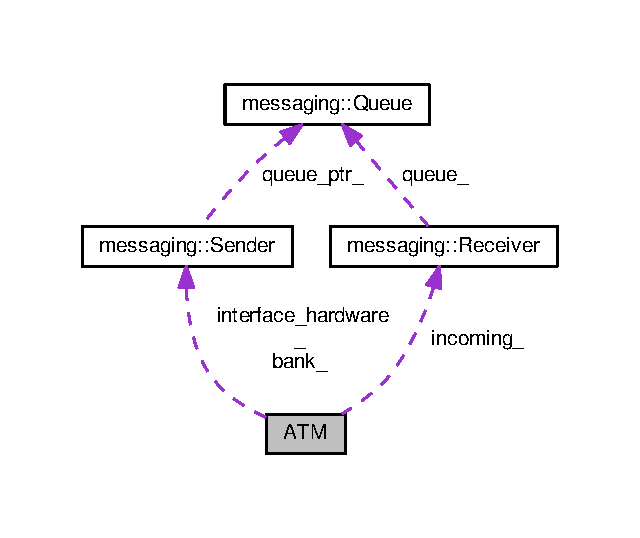
\includegraphics[width=307pt]{classATM__coll__graph}
\end{center}
\end{figure}
\subsection*{Public Member Functions}
\begin{DoxyCompactItemize}
\item 
\hyperlink{classATM_a8e0ede939f35c0a2818fdeda39ff586b}{A\-T\-M} (\hyperlink{classmessaging_1_1Sender}{messaging\-::\-Sender} bank, \hyperlink{classmessaging_1_1Sender}{messaging\-::\-Sender} interface\-\_\-hardware)
\item 
void \hyperlink{classATM_add4ca9f2b7c6ab6e0cb81cbcb925069e}{Done} ()
\item 
void \hyperlink{classATM_a03fb6655e150b1381a8aa595e4403d06}{Run} ()
\item 
\hyperlink{classmessaging_1_1Sender}{messaging\-::\-Sender} \hyperlink{classATM_a2aa23e220496bdd41d651151a1cc97e6}{Get\-Sender} ()
\end{DoxyCompactItemize}
\subsection*{Private Member Functions}
\begin{DoxyCompactItemize}
\item 
void \hyperlink{classATM_aa8ee553ff388f9977f1a504fed5eb946}{Process\-Withdrawal} ()
\item 
void \hyperlink{classATM_a4adb797522de2abb66dadd033f11a8f7}{Process\-Balance} ()
\item 
void \hyperlink{classATM_adb4a5188bec74d4cd199acdd6e62941d}{Wait\-For\-Action} ()
\item 
void \hyperlink{classATM_a1378674f5e175c6f99cccb8b848e3512}{Verifying\-Pin} ()
\item 
void \hyperlink{classATM_a2a182a5996cbed4122a9c1afd2f1697a}{Getting\-Pin} ()
\item 
void \hyperlink{classATM_ae530dbaa0e091b13f919542d002ef216}{Wait\-For\-Card} ()
\item 
void \hyperlink{classATM_accef2f77884d7272e7fe3cdfc210ba35}{Done\-Processing} ()
\end{DoxyCompactItemize}
\subsection*{Private Attributes}
\begin{DoxyCompactItemize}
\item 
\hyperlink{classmessaging_1_1Receiver}{messaging\-::\-Receiver} \hyperlink{classATM_a59b7d4c15875982aef0399de08d1c6c0}{incoming\-\_\-}
\item 
\hyperlink{classmessaging_1_1Sender}{messaging\-::\-Sender} \hyperlink{classATM_ad4f43517a9785b318afb336355672efe}{bank\-\_\-}
\item 
\hyperlink{classmessaging_1_1Sender}{messaging\-::\-Sender} \hyperlink{classATM_aeffb0e1f17d32a7dcf2f84643390e614}{interface\-\_\-hardware\-\_\-}
\item 
void(A\-T\-M\-::$\ast$ \hyperlink{classATM_ad655bcb7436d78fba4b0d16ab9a15ff1}{state\-\_\-} )()
\item 
std\-::string \hyperlink{classATM_a25cd6fda12c3a95144d820de539adee6}{account\-\_\-}
\item 
unsigned \hyperlink{classATM_a45c2bec3b3f822e15db0304d7ed26529}{withdrawal\-\_\-amount\-\_\-}
\item 
std\-::string \hyperlink{classATM_abf1480605c201cac7d94e0057c372517}{pin\-\_\-}
\end{DoxyCompactItemize}


\subsection{Constructor \& Destructor Documentation}
\hypertarget{classATM_a8e0ede939f35c0a2818fdeda39ff586b}{\index{A\-T\-M@{A\-T\-M}!A\-T\-M@{A\-T\-M}}
\index{A\-T\-M@{A\-T\-M}!ATM@{A\-T\-M}}
\subsubsection[{A\-T\-M}]{\setlength{\rightskip}{0pt plus 5cm}A\-T\-M\-::\-A\-T\-M (
\begin{DoxyParamCaption}
\item[{{\bf messaging\-::\-Sender}}]{bank, }
\item[{{\bf messaging\-::\-Sender}}]{interface\-\_\-hardware}
\end{DoxyParamCaption}
)\hspace{0.3cm}{\ttfamily [inline]}}}\label{classATM_a8e0ede939f35c0a2818fdeda39ff586b}


\subsection{Member Function Documentation}
\hypertarget{classATM_add4ca9f2b7c6ab6e0cb81cbcb925069e}{\index{A\-T\-M@{A\-T\-M}!Done@{Done}}
\index{Done@{Done}!ATM@{A\-T\-M}}
\subsubsection[{Done}]{\setlength{\rightskip}{0pt plus 5cm}void A\-T\-M\-::\-Done (
\begin{DoxyParamCaption}
{}
\end{DoxyParamCaption}
)\hspace{0.3cm}{\ttfamily [inline]}}}\label{classATM_add4ca9f2b7c6ab6e0cb81cbcb925069e}


Here is the call graph for this function\-:\nopagebreak
\begin{figure}[H]
\begin{center}
\leavevmode
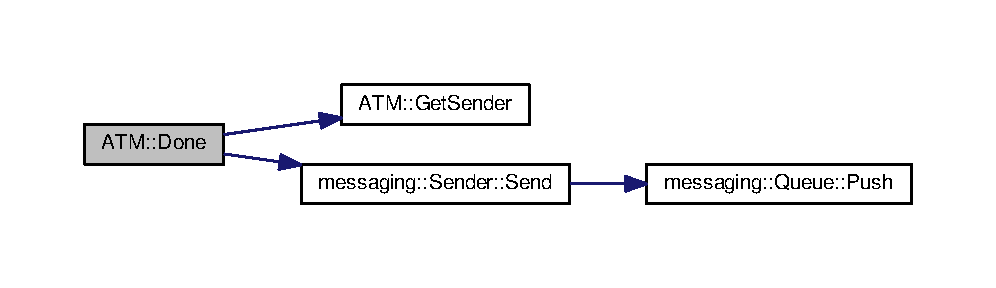
\includegraphics[width=350pt]{classATM_add4ca9f2b7c6ab6e0cb81cbcb925069e_cgraph}
\end{center}
\end{figure}


\hypertarget{classATM_accef2f77884d7272e7fe3cdfc210ba35}{\index{A\-T\-M@{A\-T\-M}!Done\-Processing@{Done\-Processing}}
\index{Done\-Processing@{Done\-Processing}!ATM@{A\-T\-M}}
\subsubsection[{Done\-Processing}]{\setlength{\rightskip}{0pt plus 5cm}void A\-T\-M\-::\-Done\-Processing (
\begin{DoxyParamCaption}
{}
\end{DoxyParamCaption}
)\hspace{0.3cm}{\ttfamily [inline]}, {\ttfamily [private]}}}\label{classATM_accef2f77884d7272e7fe3cdfc210ba35}


Here is the call graph for this function\-:
\nopagebreak
\begin{figure}[H]
\begin{center}
\leavevmode
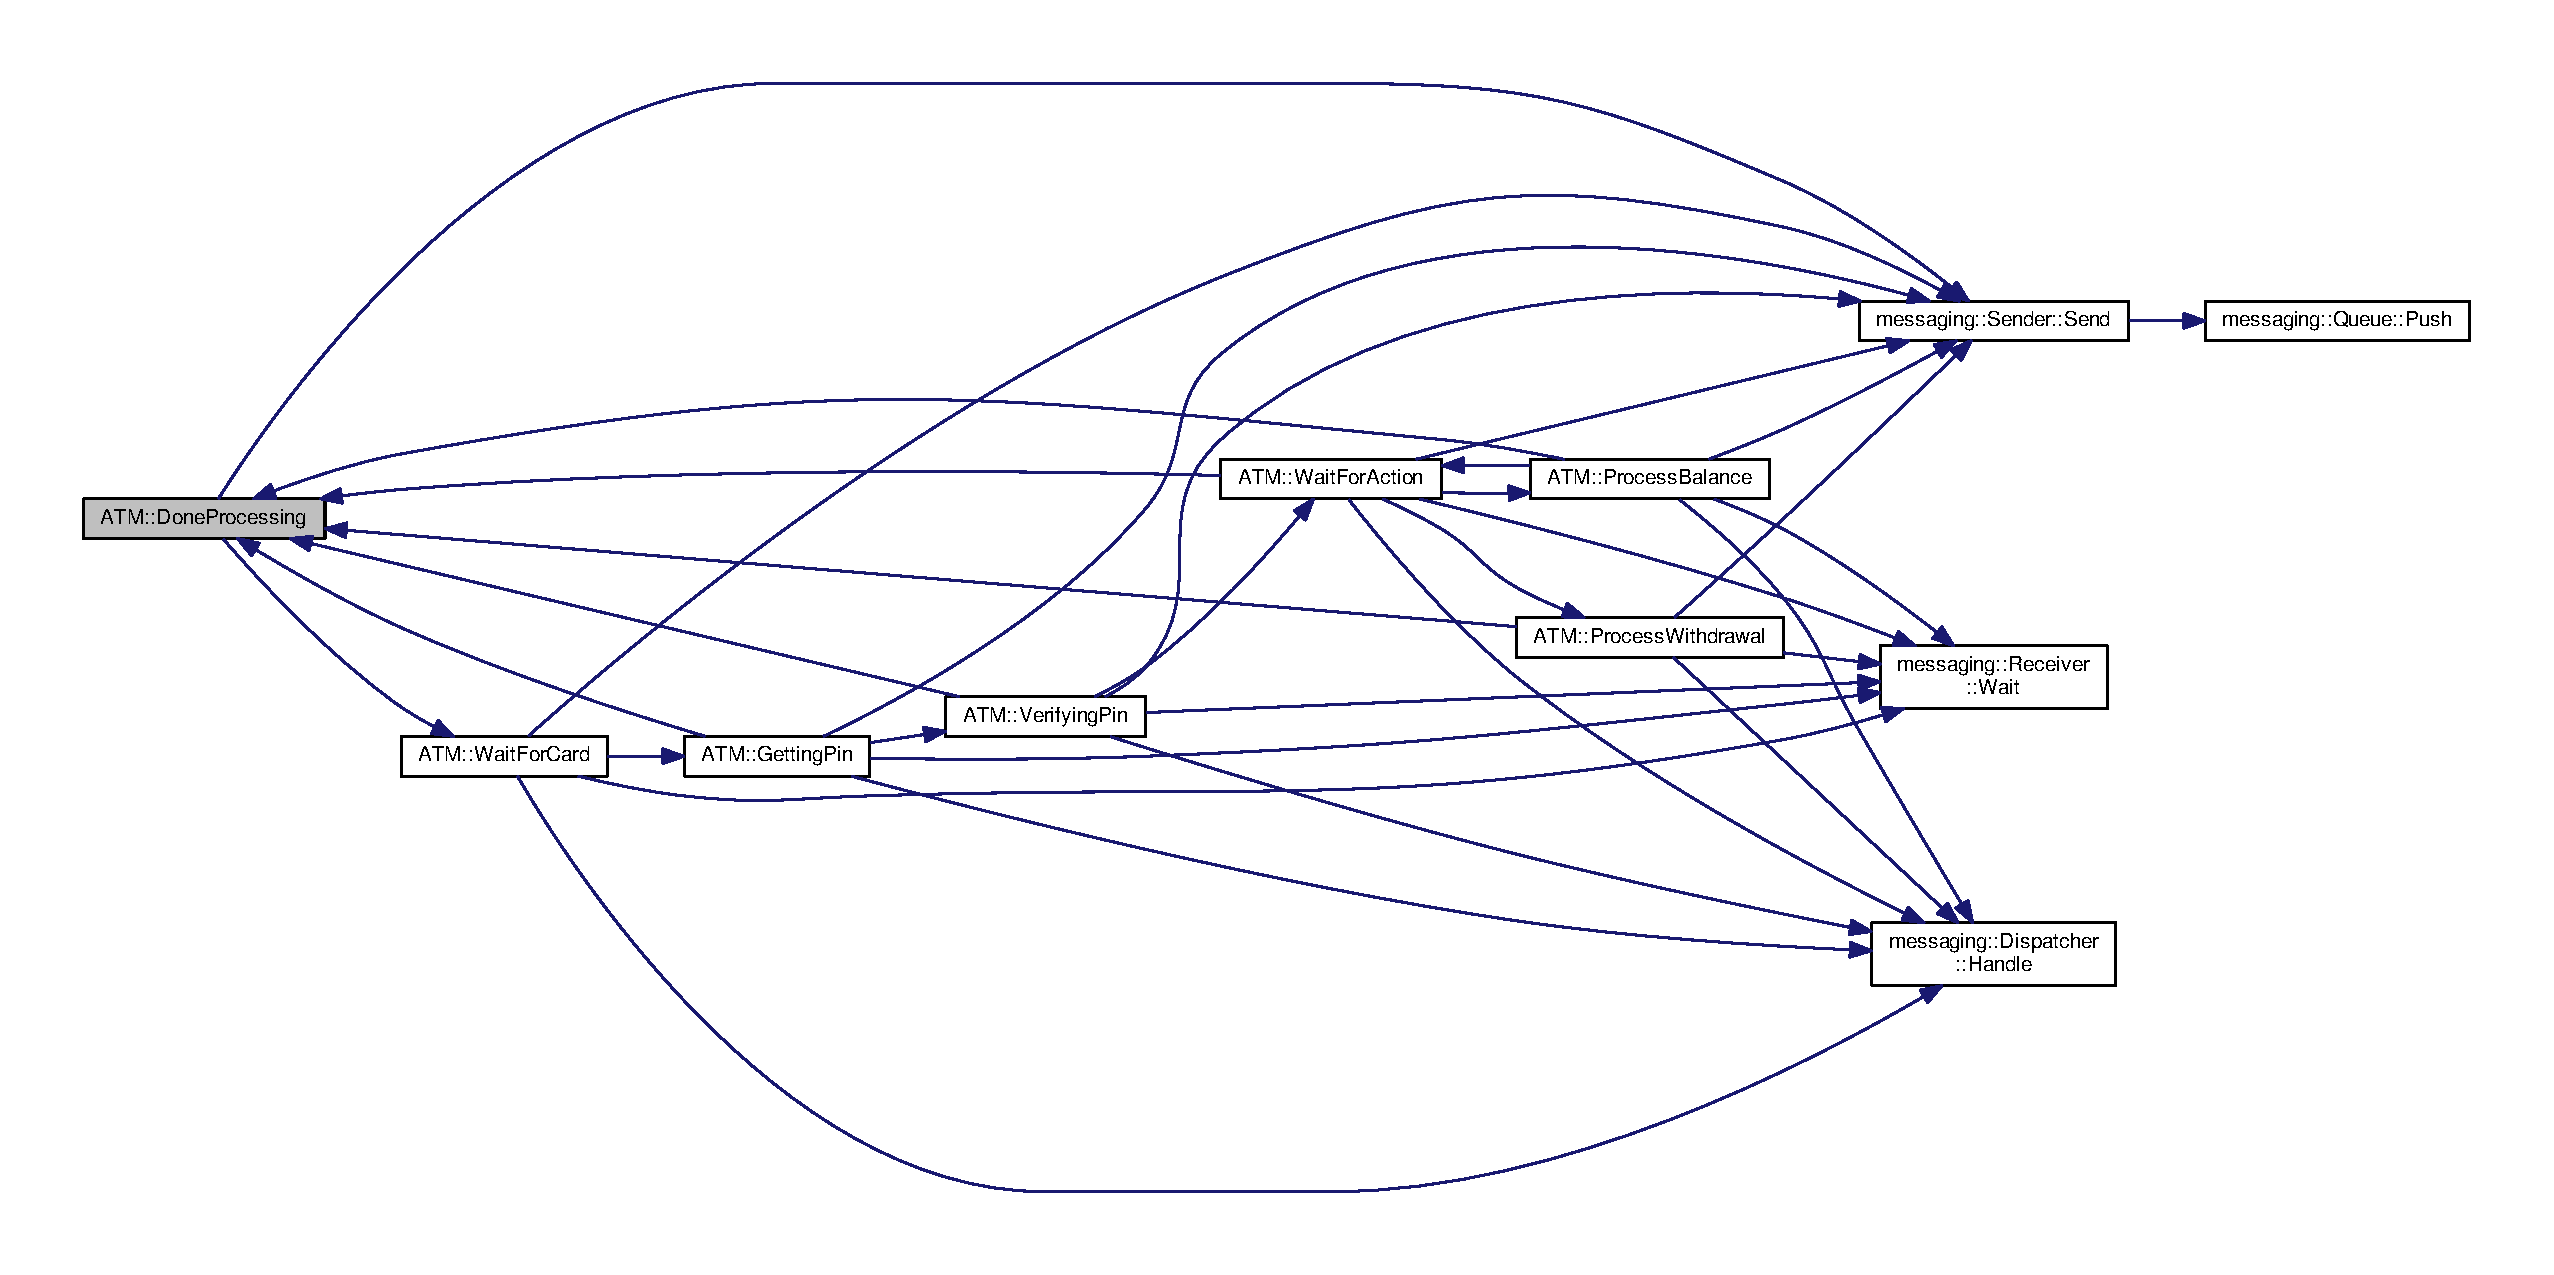
\includegraphics[width=350pt]{classATM_accef2f77884d7272e7fe3cdfc210ba35_cgraph}
\end{center}
\end{figure}


\hypertarget{classATM_a2aa23e220496bdd41d651151a1cc97e6}{\index{A\-T\-M@{A\-T\-M}!Get\-Sender@{Get\-Sender}}
\index{Get\-Sender@{Get\-Sender}!ATM@{A\-T\-M}}
\subsubsection[{Get\-Sender}]{\setlength{\rightskip}{0pt plus 5cm}{\bf messaging\-::\-Sender} A\-T\-M\-::\-Get\-Sender (
\begin{DoxyParamCaption}
{}
\end{DoxyParamCaption}
)\hspace{0.3cm}{\ttfamily [inline]}}}\label{classATM_a2aa23e220496bdd41d651151a1cc97e6}
\hypertarget{classATM_a2a182a5996cbed4122a9c1afd2f1697a}{\index{A\-T\-M@{A\-T\-M}!Getting\-Pin@{Getting\-Pin}}
\index{Getting\-Pin@{Getting\-Pin}!ATM@{A\-T\-M}}
\subsubsection[{Getting\-Pin}]{\setlength{\rightskip}{0pt plus 5cm}void A\-T\-M\-::\-Getting\-Pin (
\begin{DoxyParamCaption}
{}
\end{DoxyParamCaption}
)\hspace{0.3cm}{\ttfamily [inline]}, {\ttfamily [private]}}}\label{classATM_a2a182a5996cbed4122a9c1afd2f1697a}


Here is the call graph for this function\-:
\nopagebreak
\begin{figure}[H]
\begin{center}
\leavevmode
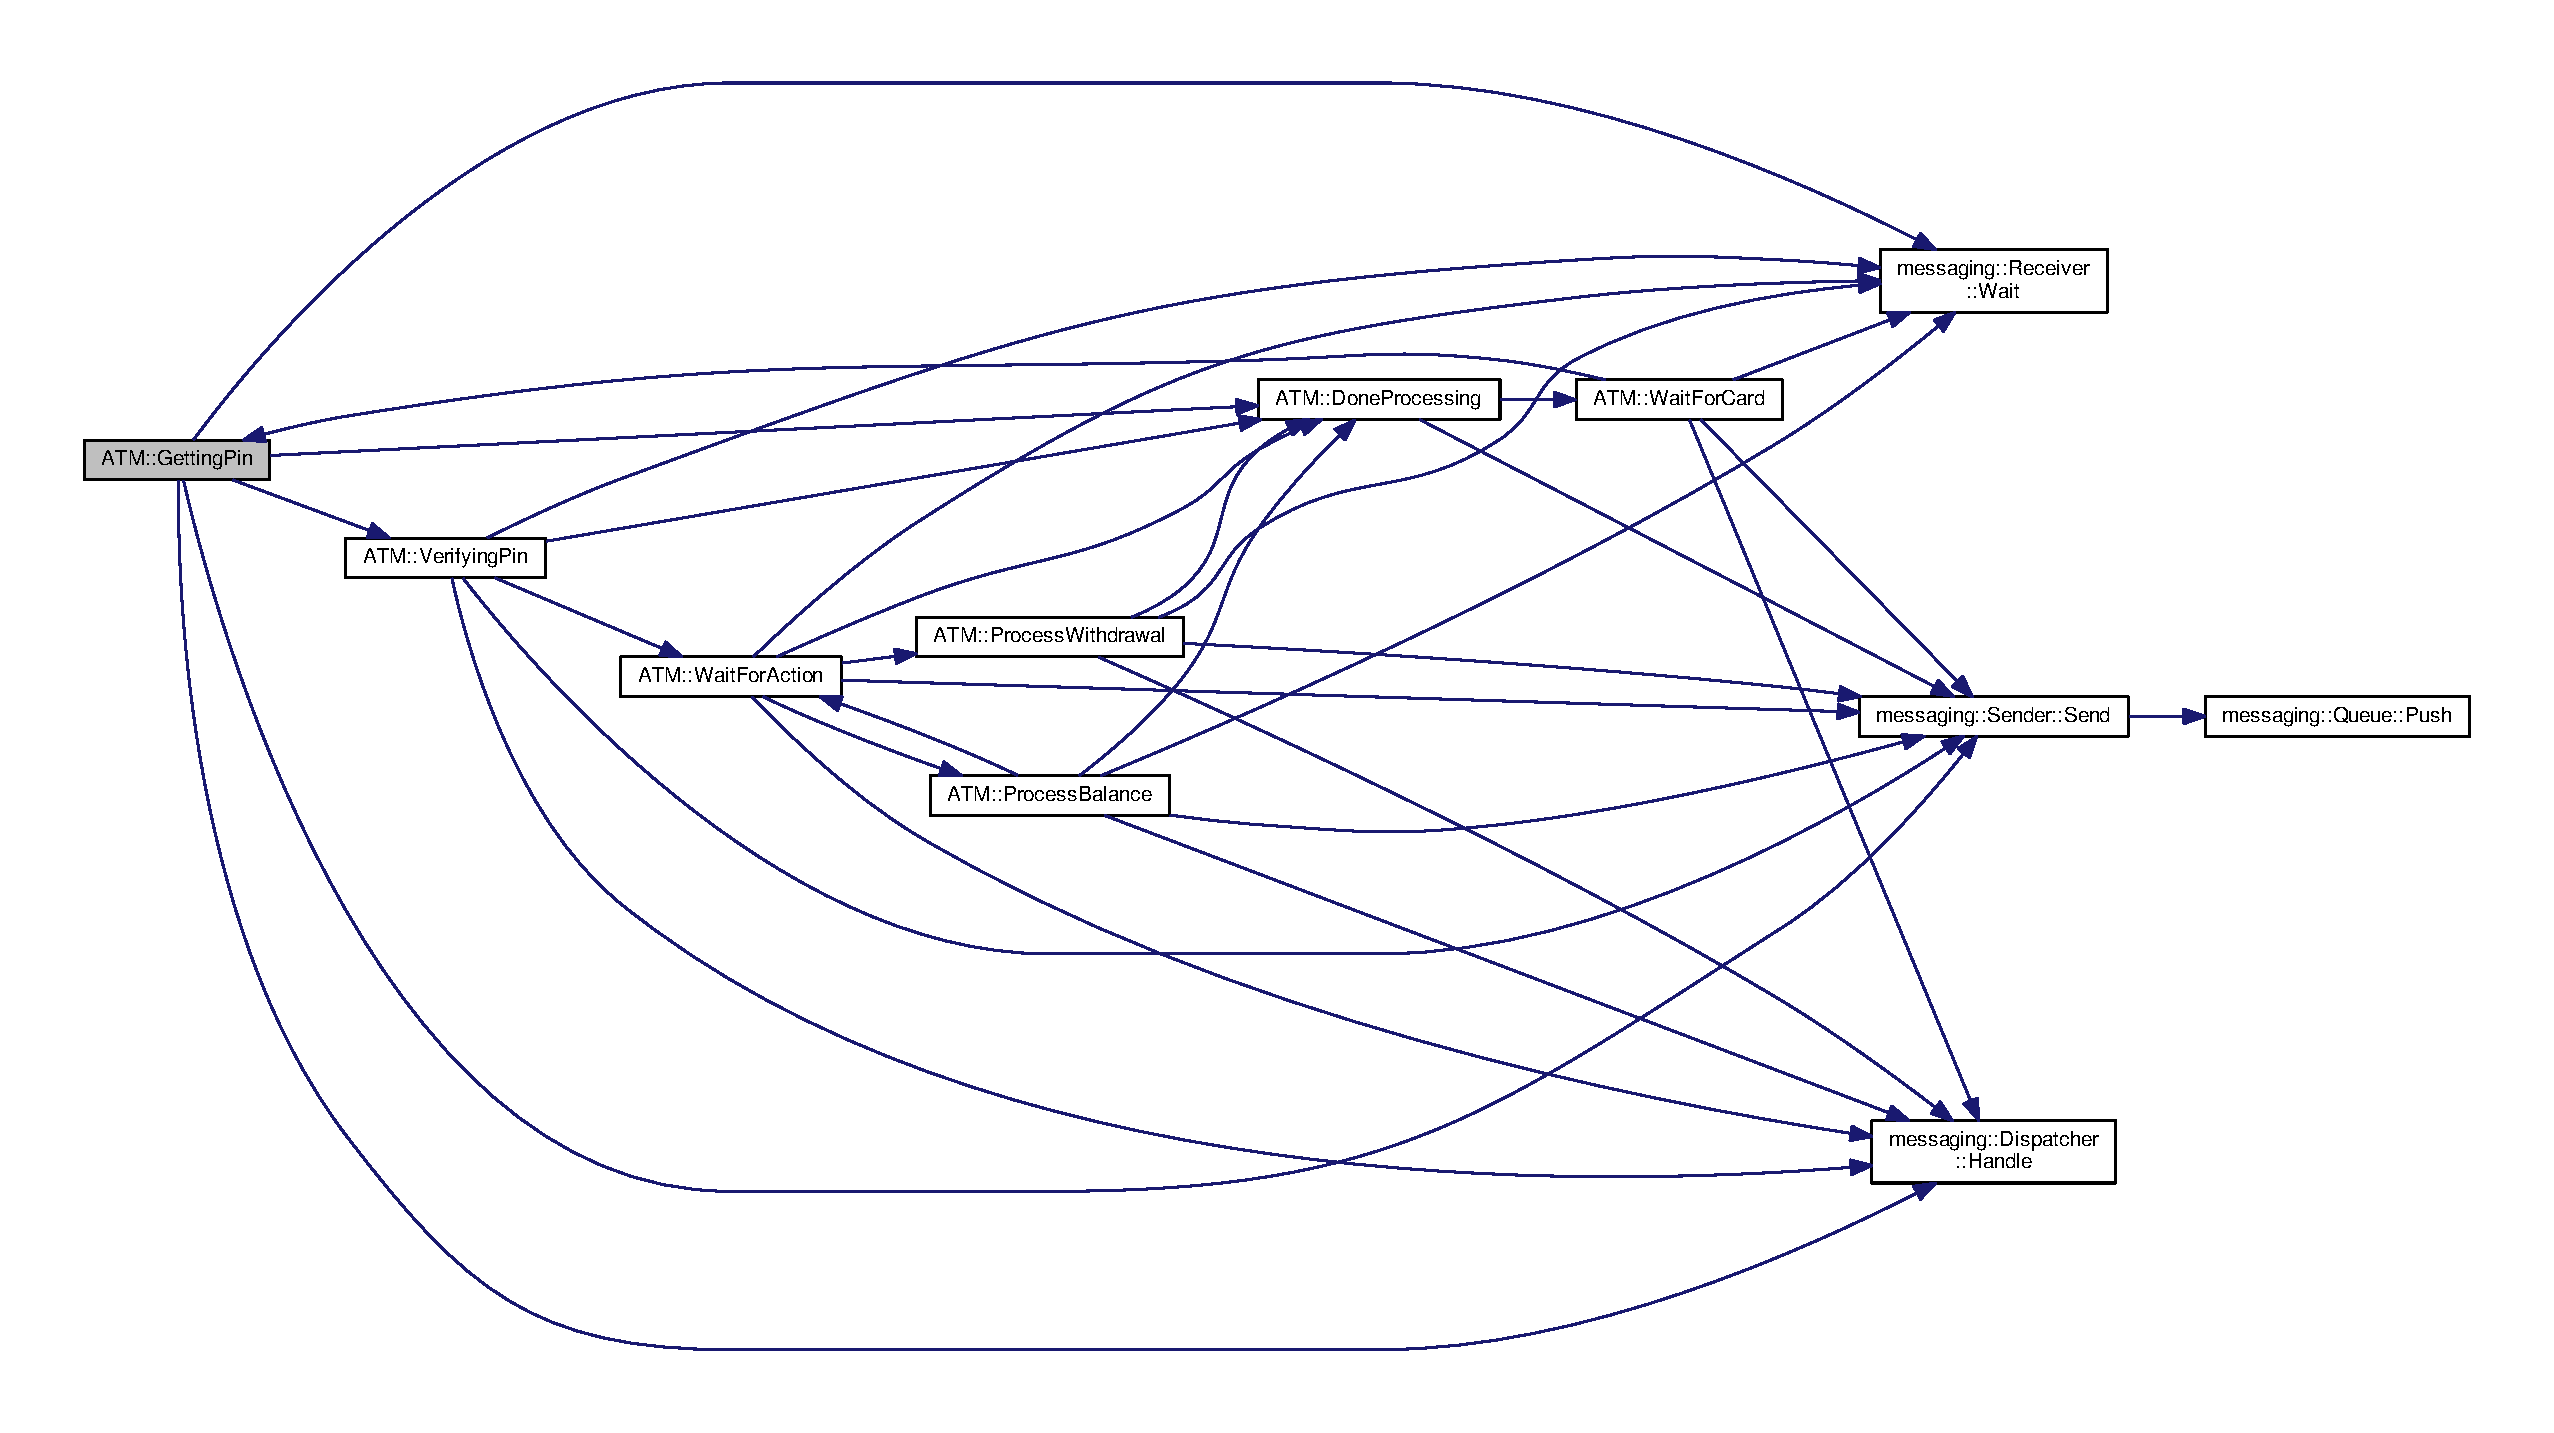
\includegraphics[width=350pt]{classATM_a2a182a5996cbed4122a9c1afd2f1697a_cgraph}
\end{center}
\end{figure}


\hypertarget{classATM_a4adb797522de2abb66dadd033f11a8f7}{\index{A\-T\-M@{A\-T\-M}!Process\-Balance@{Process\-Balance}}
\index{Process\-Balance@{Process\-Balance}!ATM@{A\-T\-M}}
\subsubsection[{Process\-Balance}]{\setlength{\rightskip}{0pt plus 5cm}void A\-T\-M\-::\-Process\-Balance (
\begin{DoxyParamCaption}
{}
\end{DoxyParamCaption}
)\hspace{0.3cm}{\ttfamily [inline]}, {\ttfamily [private]}}}\label{classATM_a4adb797522de2abb66dadd033f11a8f7}


Here is the call graph for this function\-:
\nopagebreak
\begin{figure}[H]
\begin{center}
\leavevmode
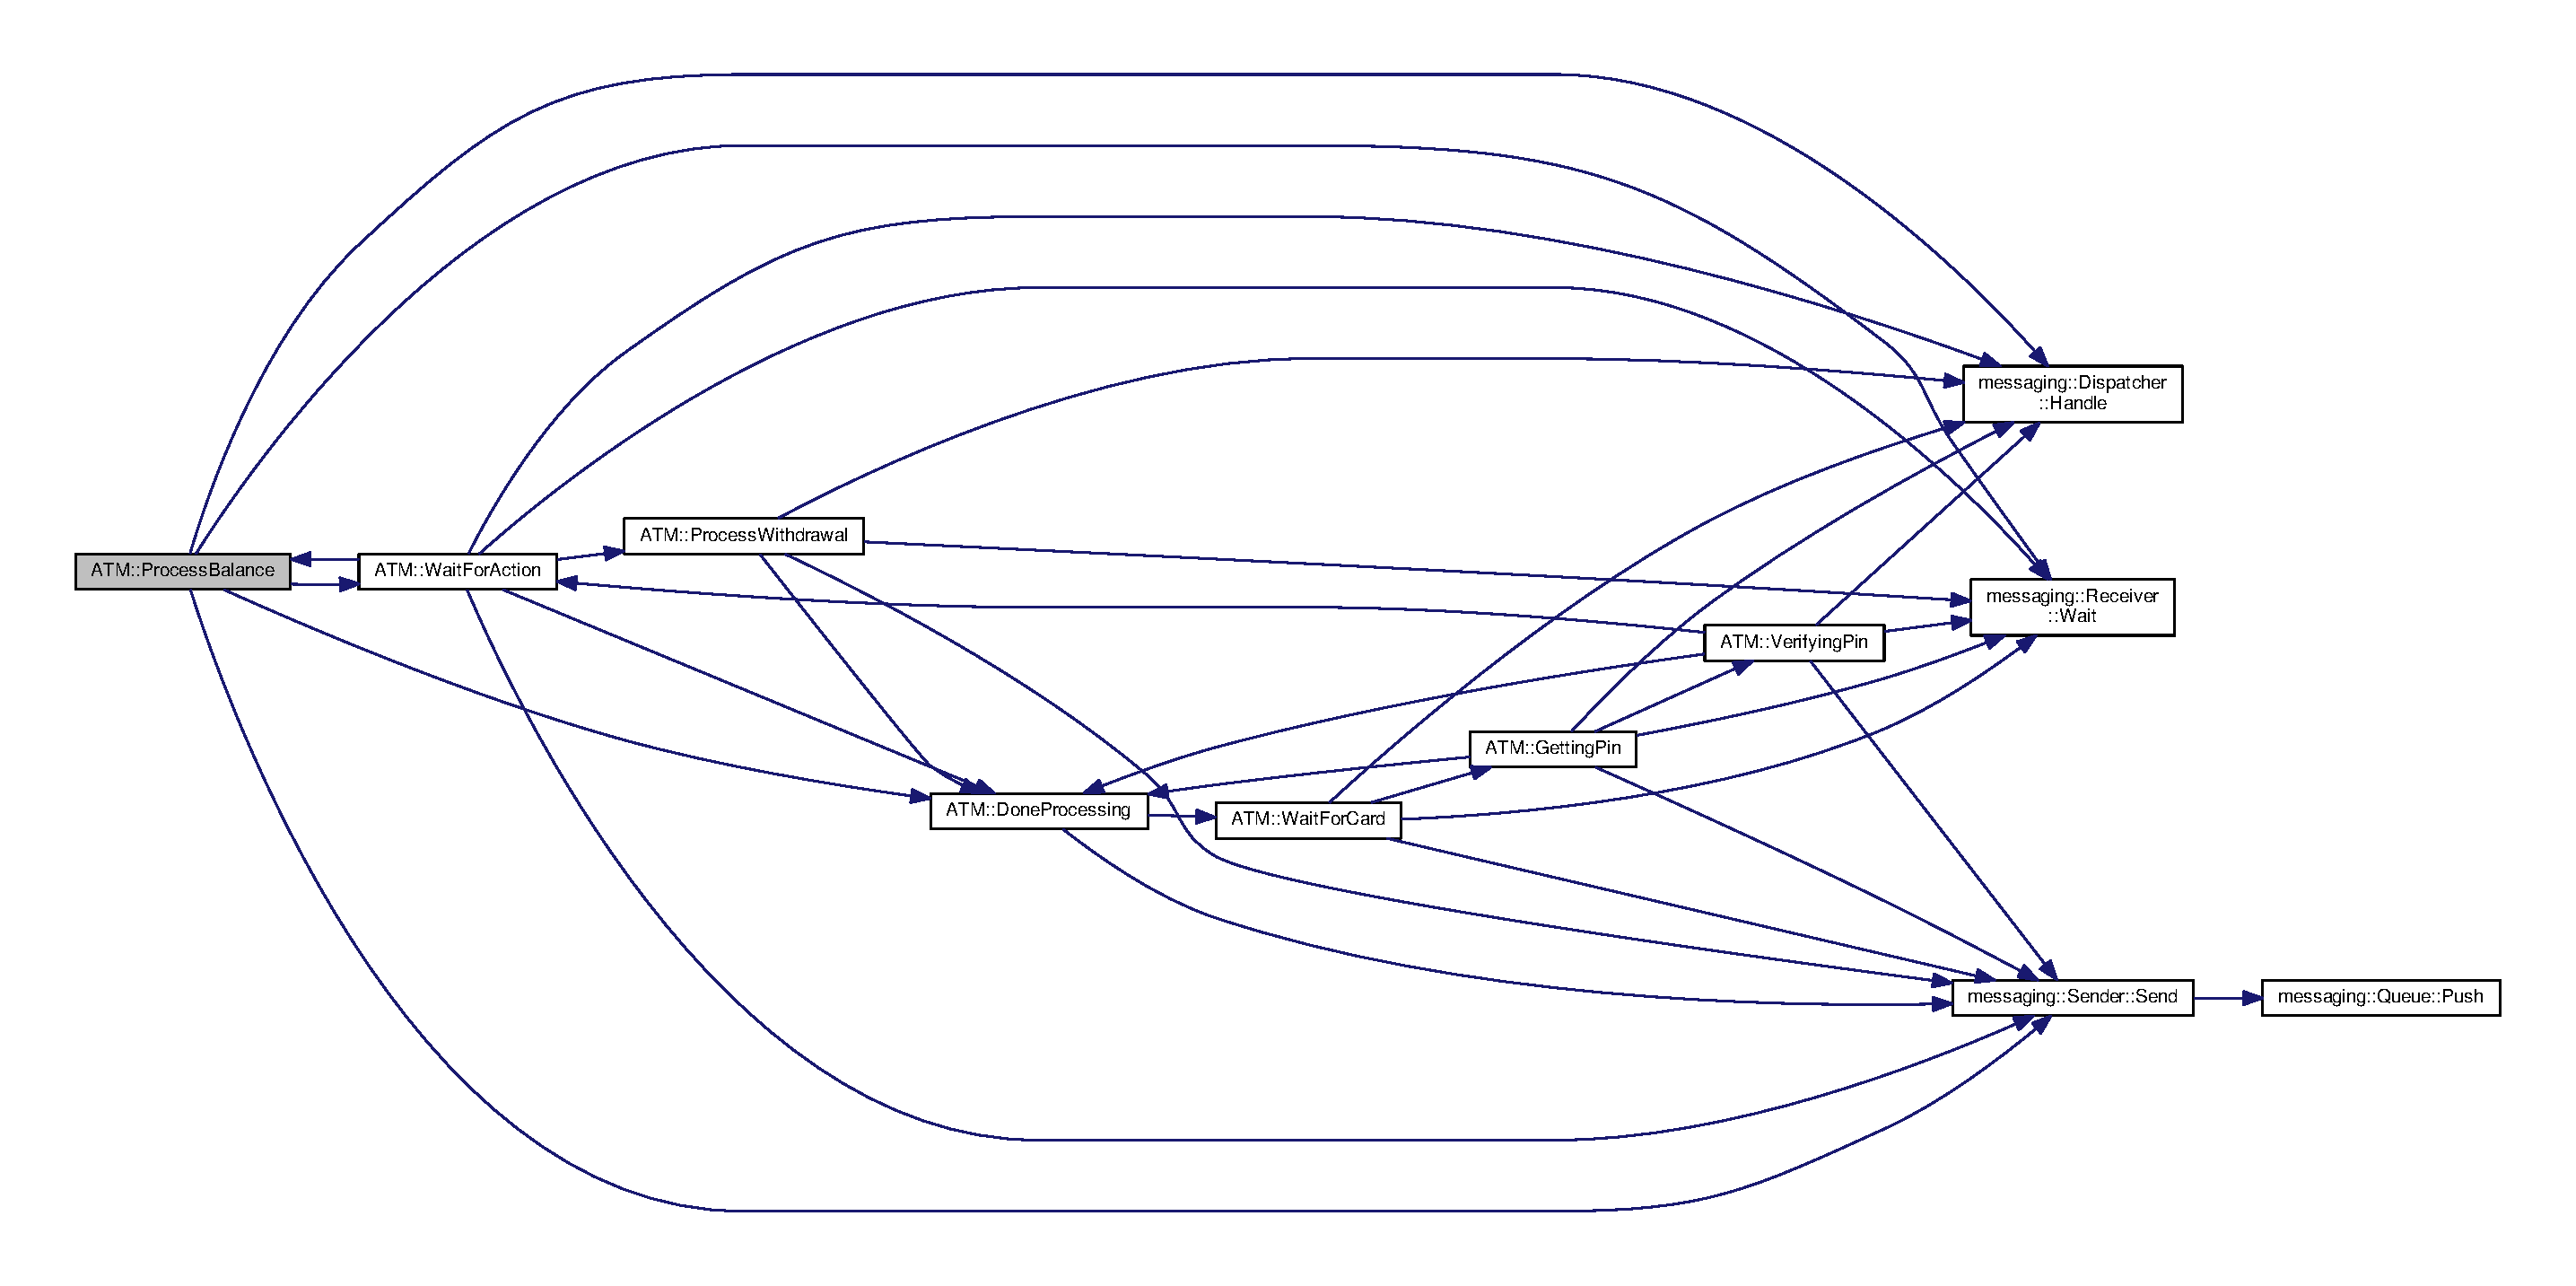
\includegraphics[width=350pt]{classATM_a4adb797522de2abb66dadd033f11a8f7_cgraph}
\end{center}
\end{figure}


\hypertarget{classATM_aa8ee553ff388f9977f1a504fed5eb946}{\index{A\-T\-M@{A\-T\-M}!Process\-Withdrawal@{Process\-Withdrawal}}
\index{Process\-Withdrawal@{Process\-Withdrawal}!ATM@{A\-T\-M}}
\subsubsection[{Process\-Withdrawal}]{\setlength{\rightskip}{0pt plus 5cm}void A\-T\-M\-::\-Process\-Withdrawal (
\begin{DoxyParamCaption}
{}
\end{DoxyParamCaption}
)\hspace{0.3cm}{\ttfamily [inline]}, {\ttfamily [private]}}}\label{classATM_aa8ee553ff388f9977f1a504fed5eb946}


Here is the call graph for this function\-:
\nopagebreak
\begin{figure}[H]
\begin{center}
\leavevmode
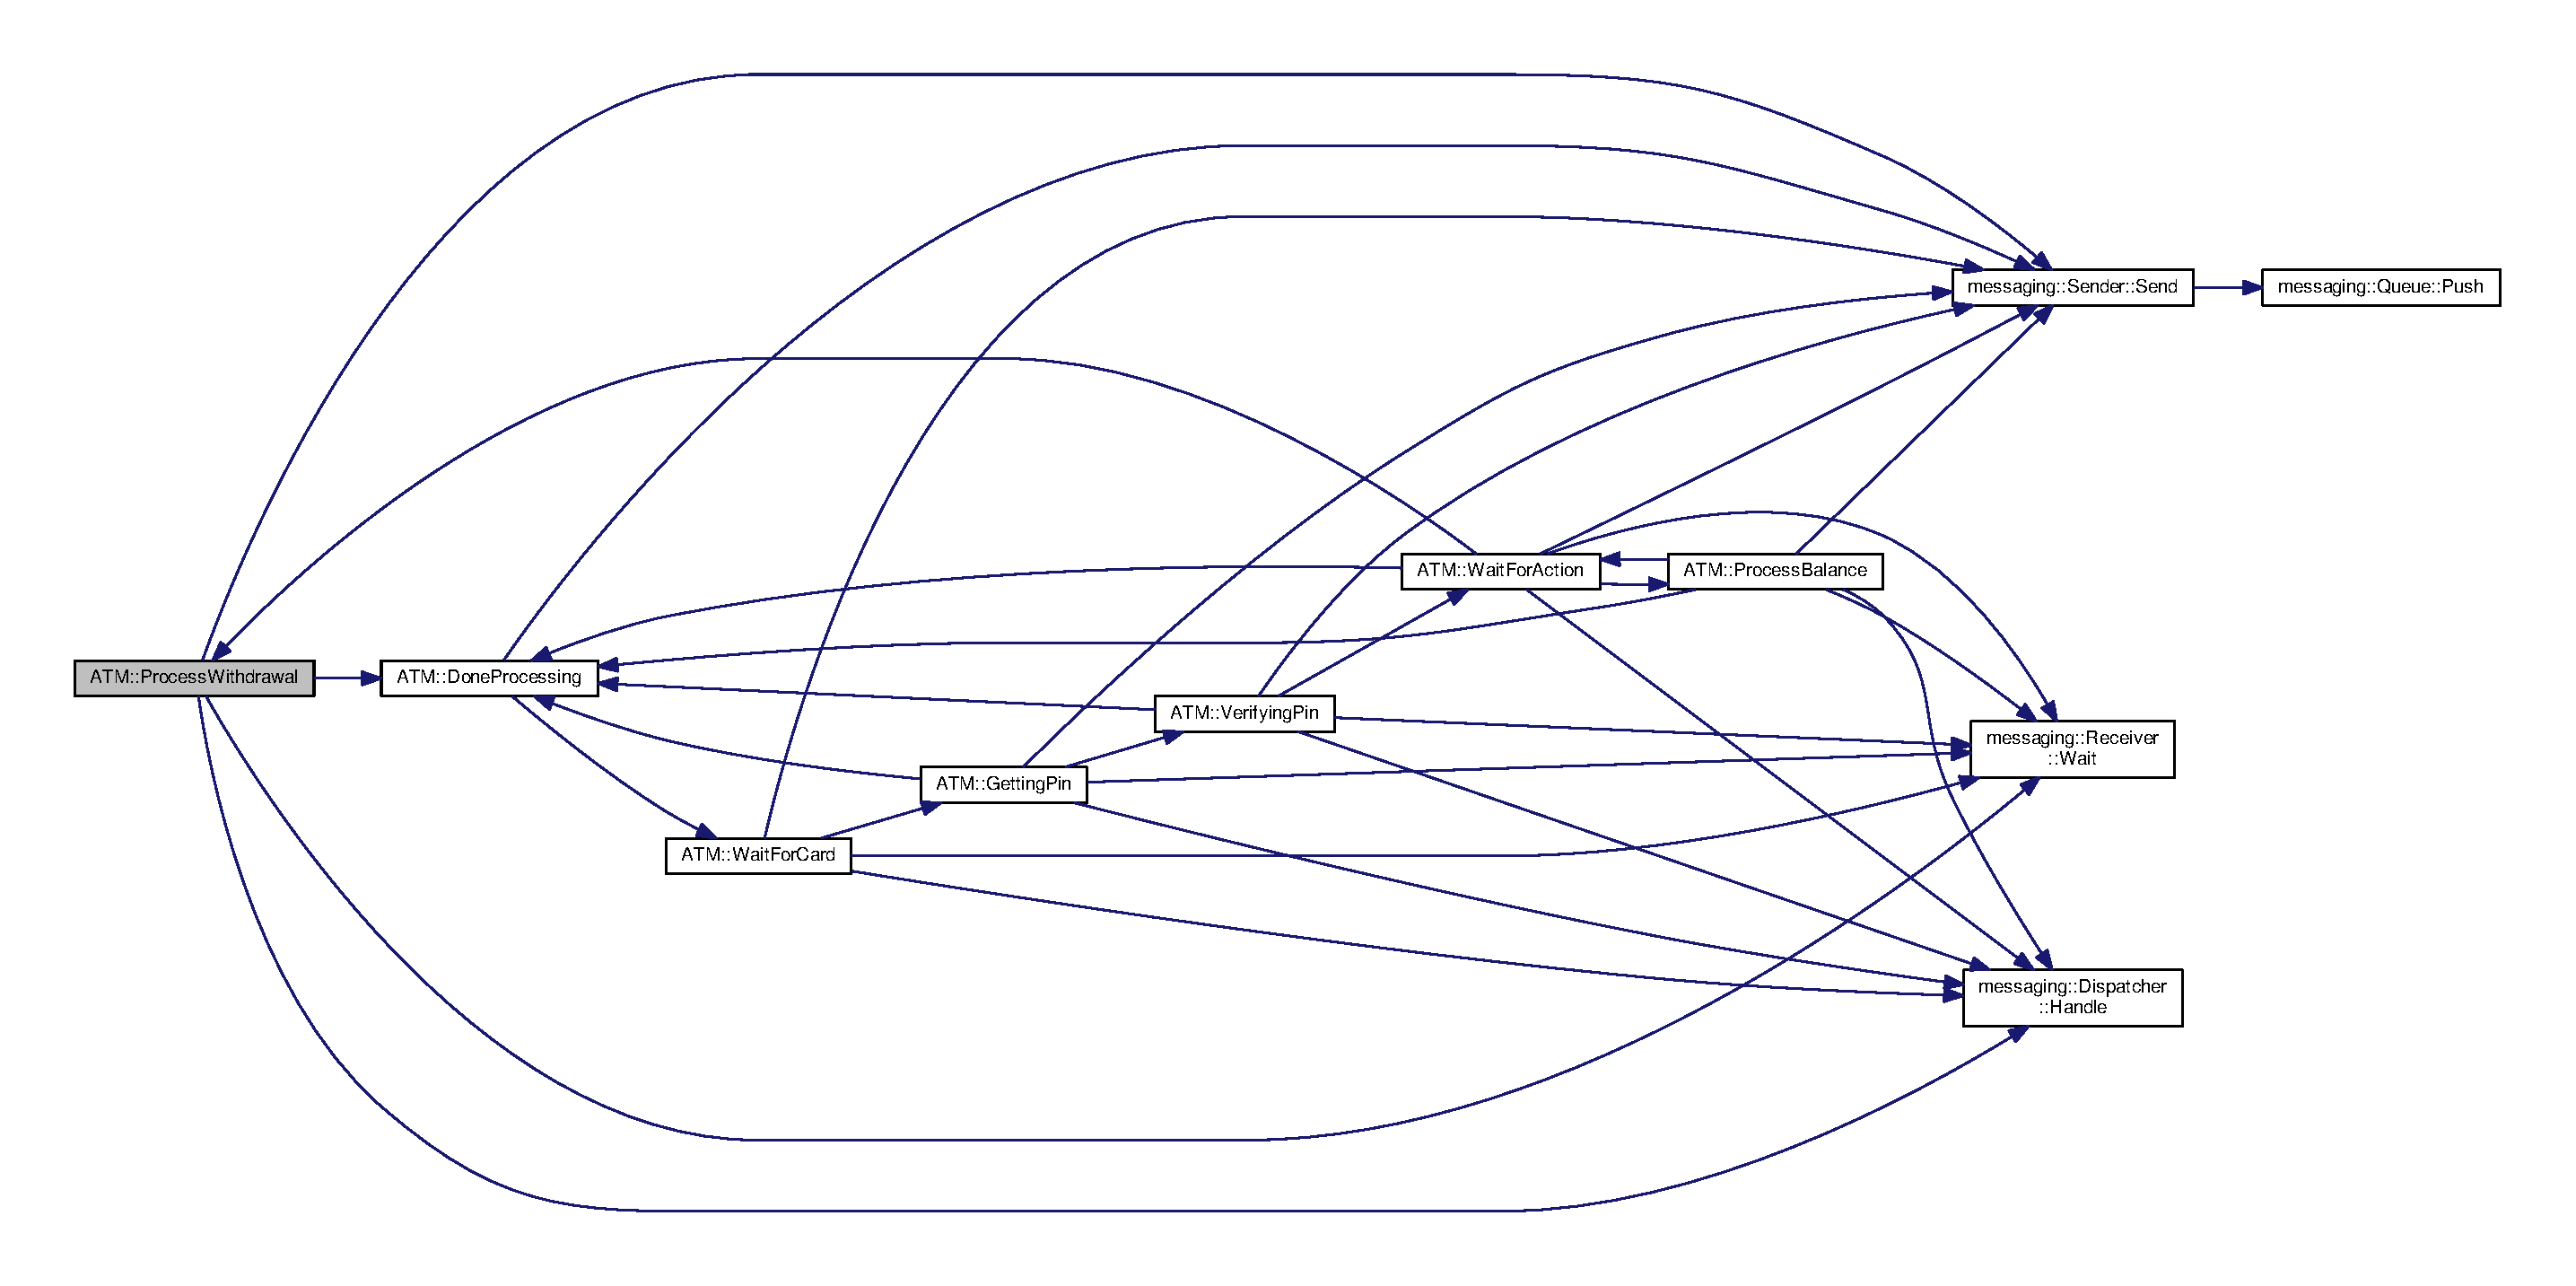
\includegraphics[width=350pt]{classATM_aa8ee553ff388f9977f1a504fed5eb946_cgraph}
\end{center}
\end{figure}


\hypertarget{classATM_a03fb6655e150b1381a8aa595e4403d06}{\index{A\-T\-M@{A\-T\-M}!Run@{Run}}
\index{Run@{Run}!ATM@{A\-T\-M}}
\subsubsection[{Run}]{\setlength{\rightskip}{0pt plus 5cm}void A\-T\-M\-::\-Run (
\begin{DoxyParamCaption}
{}
\end{DoxyParamCaption}
)\hspace{0.3cm}{\ttfamily [inline]}}}\label{classATM_a03fb6655e150b1381a8aa595e4403d06}


Here is the call graph for this function\-:
\nopagebreak
\begin{figure}[H]
\begin{center}
\leavevmode
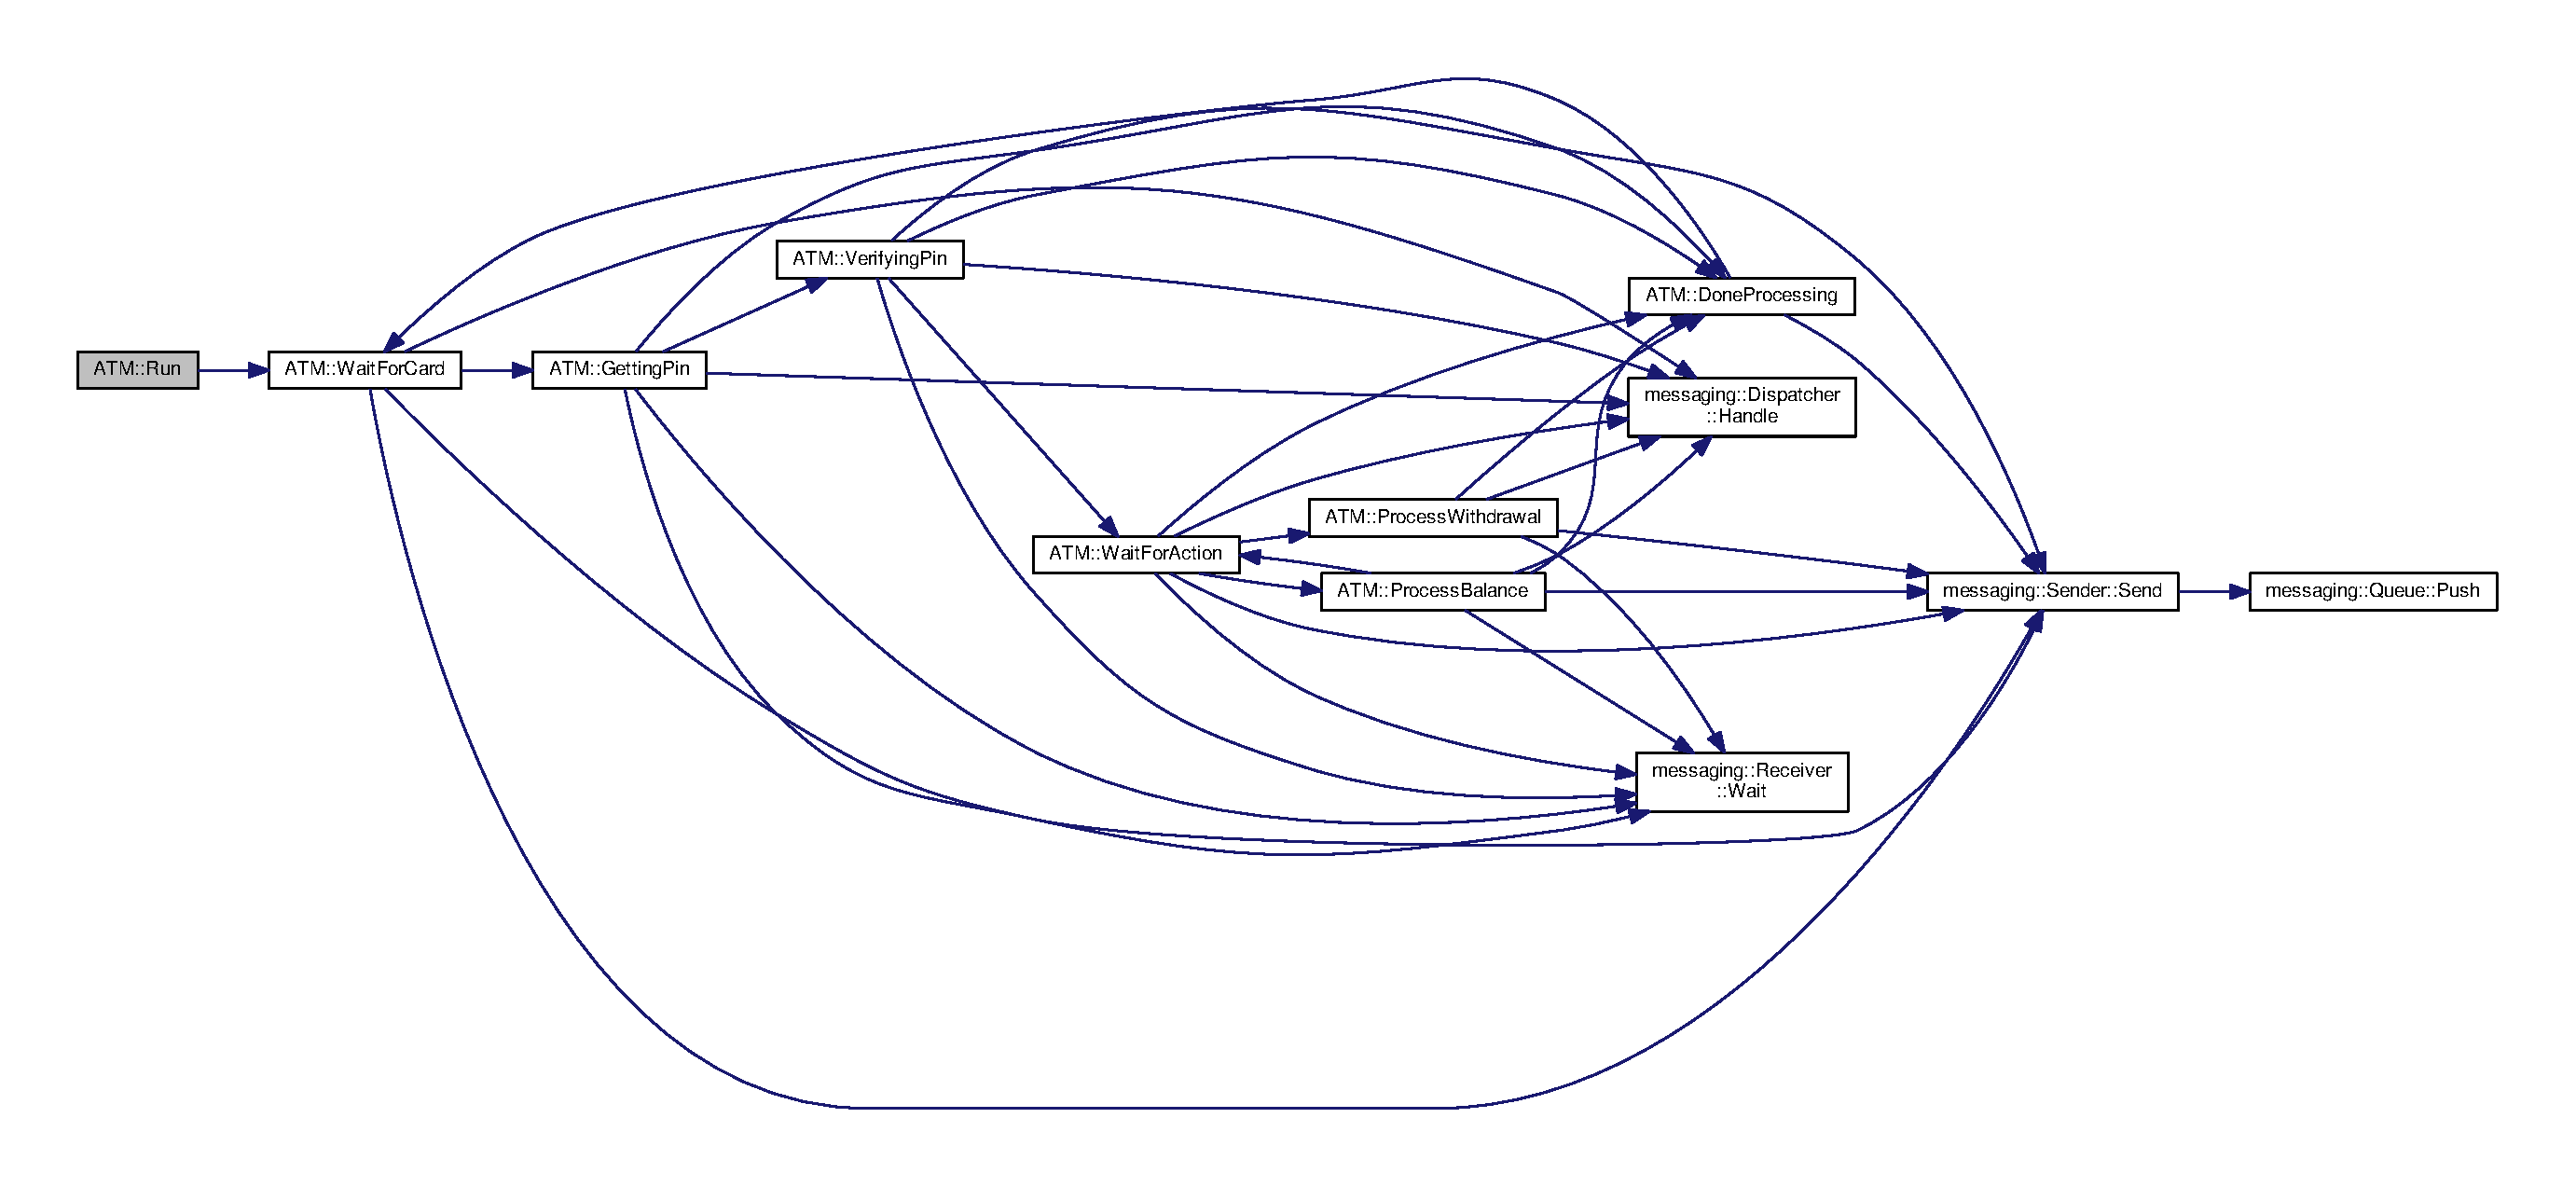
\includegraphics[width=350pt]{classATM_a03fb6655e150b1381a8aa595e4403d06_cgraph}
\end{center}
\end{figure}


\hypertarget{classATM_a1378674f5e175c6f99cccb8b848e3512}{\index{A\-T\-M@{A\-T\-M}!Verifying\-Pin@{Verifying\-Pin}}
\index{Verifying\-Pin@{Verifying\-Pin}!ATM@{A\-T\-M}}
\subsubsection[{Verifying\-Pin}]{\setlength{\rightskip}{0pt plus 5cm}void A\-T\-M\-::\-Verifying\-Pin (
\begin{DoxyParamCaption}
{}
\end{DoxyParamCaption}
)\hspace{0.3cm}{\ttfamily [inline]}, {\ttfamily [private]}}}\label{classATM_a1378674f5e175c6f99cccb8b848e3512}


Here is the call graph for this function\-:
\nopagebreak
\begin{figure}[H]
\begin{center}
\leavevmode
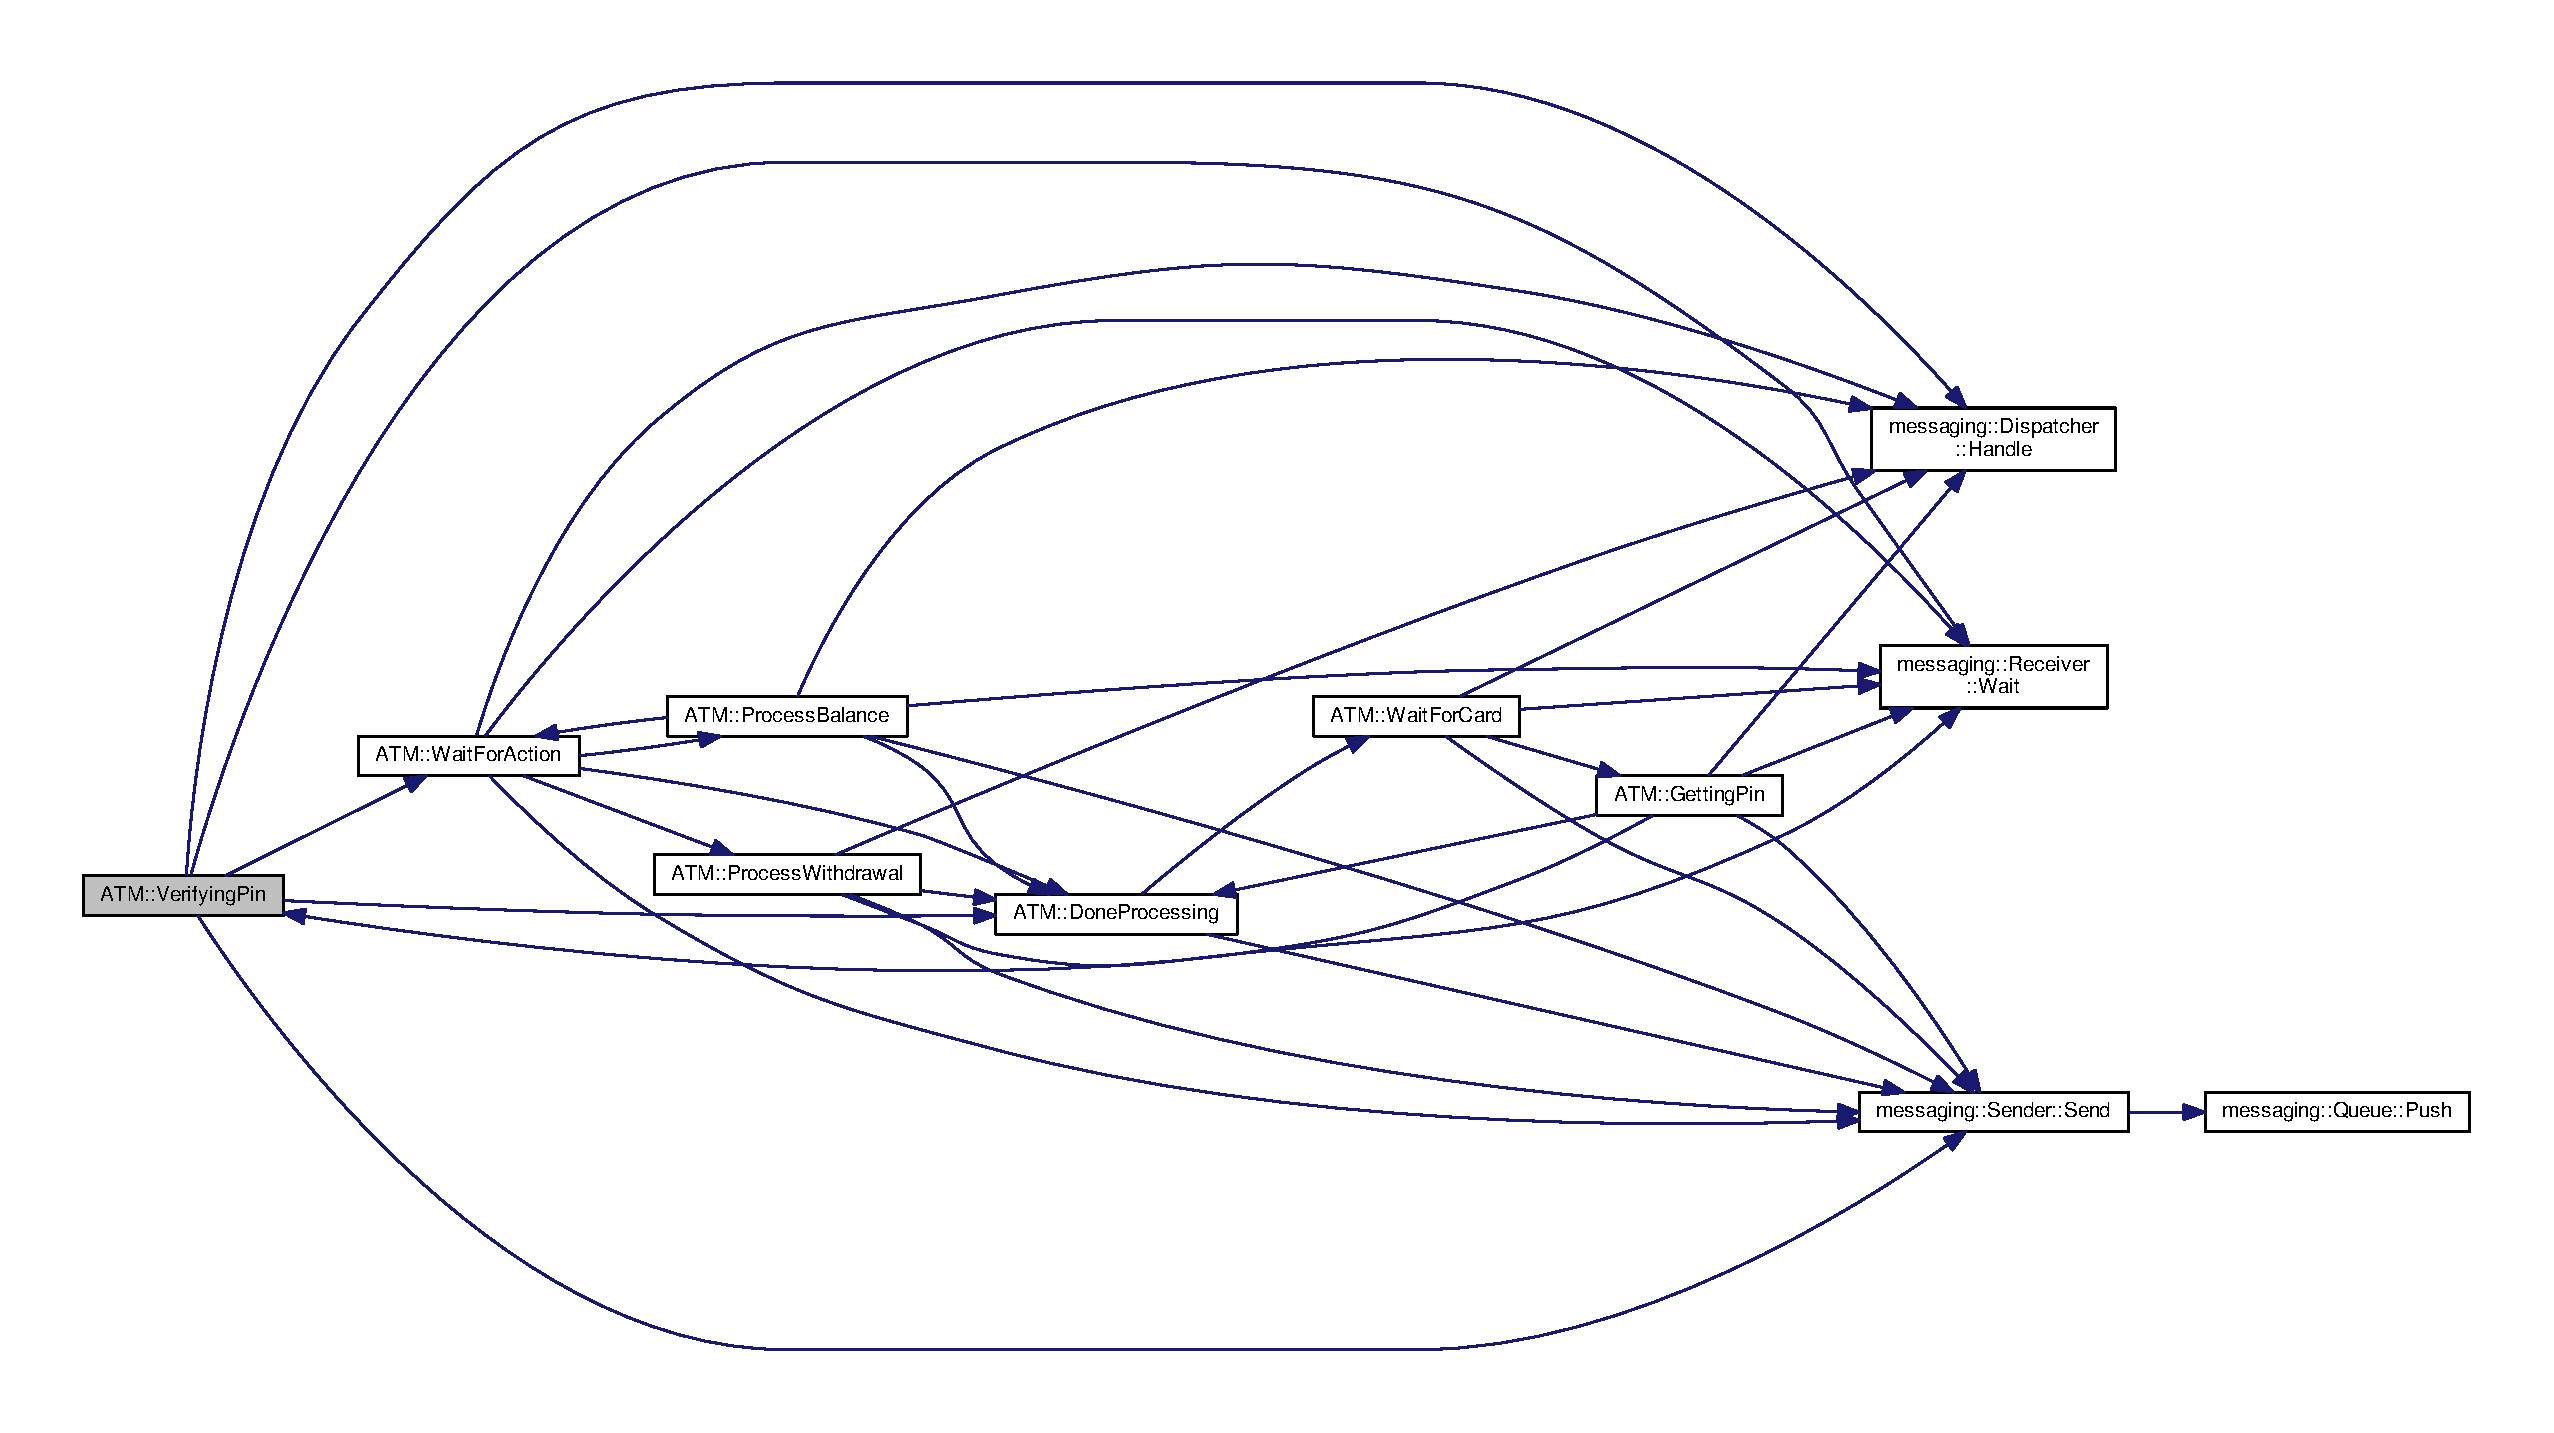
\includegraphics[width=350pt]{classATM_a1378674f5e175c6f99cccb8b848e3512_cgraph}
\end{center}
\end{figure}


\hypertarget{classATM_adb4a5188bec74d4cd199acdd6e62941d}{\index{A\-T\-M@{A\-T\-M}!Wait\-For\-Action@{Wait\-For\-Action}}
\index{Wait\-For\-Action@{Wait\-For\-Action}!ATM@{A\-T\-M}}
\subsubsection[{Wait\-For\-Action}]{\setlength{\rightskip}{0pt plus 5cm}void A\-T\-M\-::\-Wait\-For\-Action (
\begin{DoxyParamCaption}
{}
\end{DoxyParamCaption}
)\hspace{0.3cm}{\ttfamily [inline]}, {\ttfamily [private]}}}\label{classATM_adb4a5188bec74d4cd199acdd6e62941d}


Here is the call graph for this function\-:
\nopagebreak
\begin{figure}[H]
\begin{center}
\leavevmode
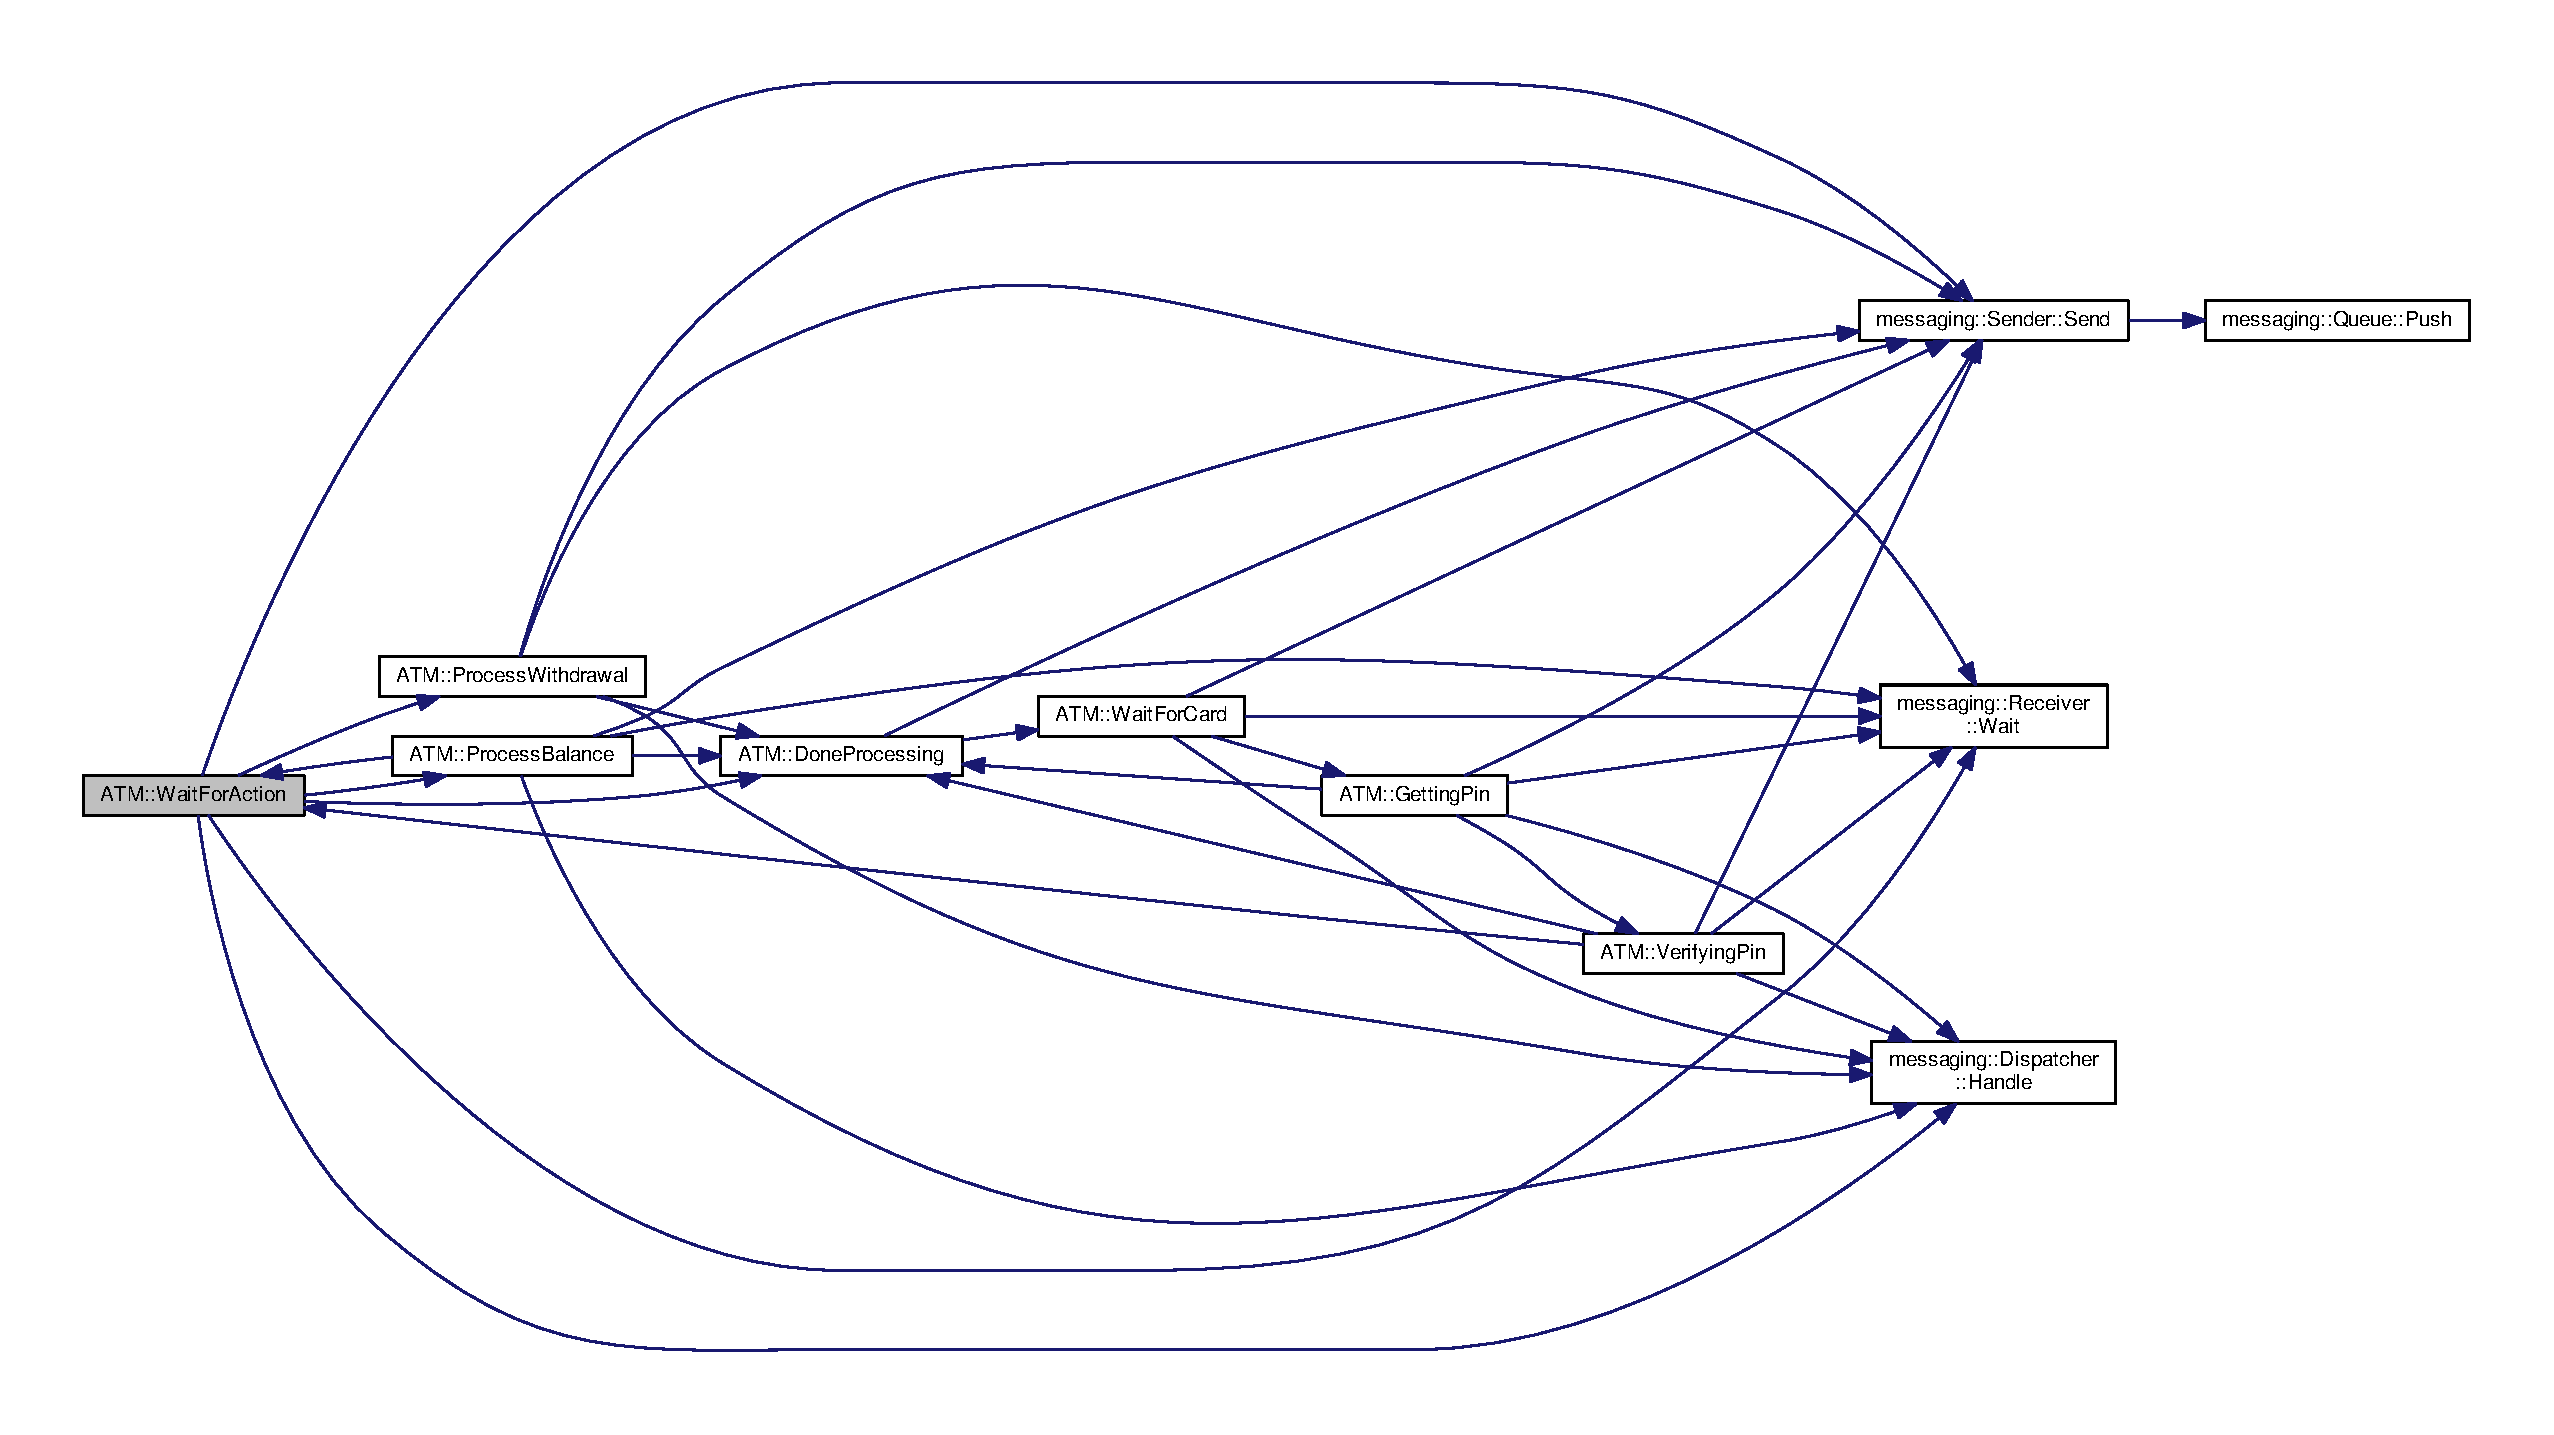
\includegraphics[width=350pt]{classATM_adb4a5188bec74d4cd199acdd6e62941d_cgraph}
\end{center}
\end{figure}


\hypertarget{classATM_ae530dbaa0e091b13f919542d002ef216}{\index{A\-T\-M@{A\-T\-M}!Wait\-For\-Card@{Wait\-For\-Card}}
\index{Wait\-For\-Card@{Wait\-For\-Card}!ATM@{A\-T\-M}}
\subsubsection[{Wait\-For\-Card}]{\setlength{\rightskip}{0pt plus 5cm}void A\-T\-M\-::\-Wait\-For\-Card (
\begin{DoxyParamCaption}
{}
\end{DoxyParamCaption}
)\hspace{0.3cm}{\ttfamily [inline]}, {\ttfamily [private]}}}\label{classATM_ae530dbaa0e091b13f919542d002ef216}


Here is the call graph for this function\-:
\nopagebreak
\begin{figure}[H]
\begin{center}
\leavevmode
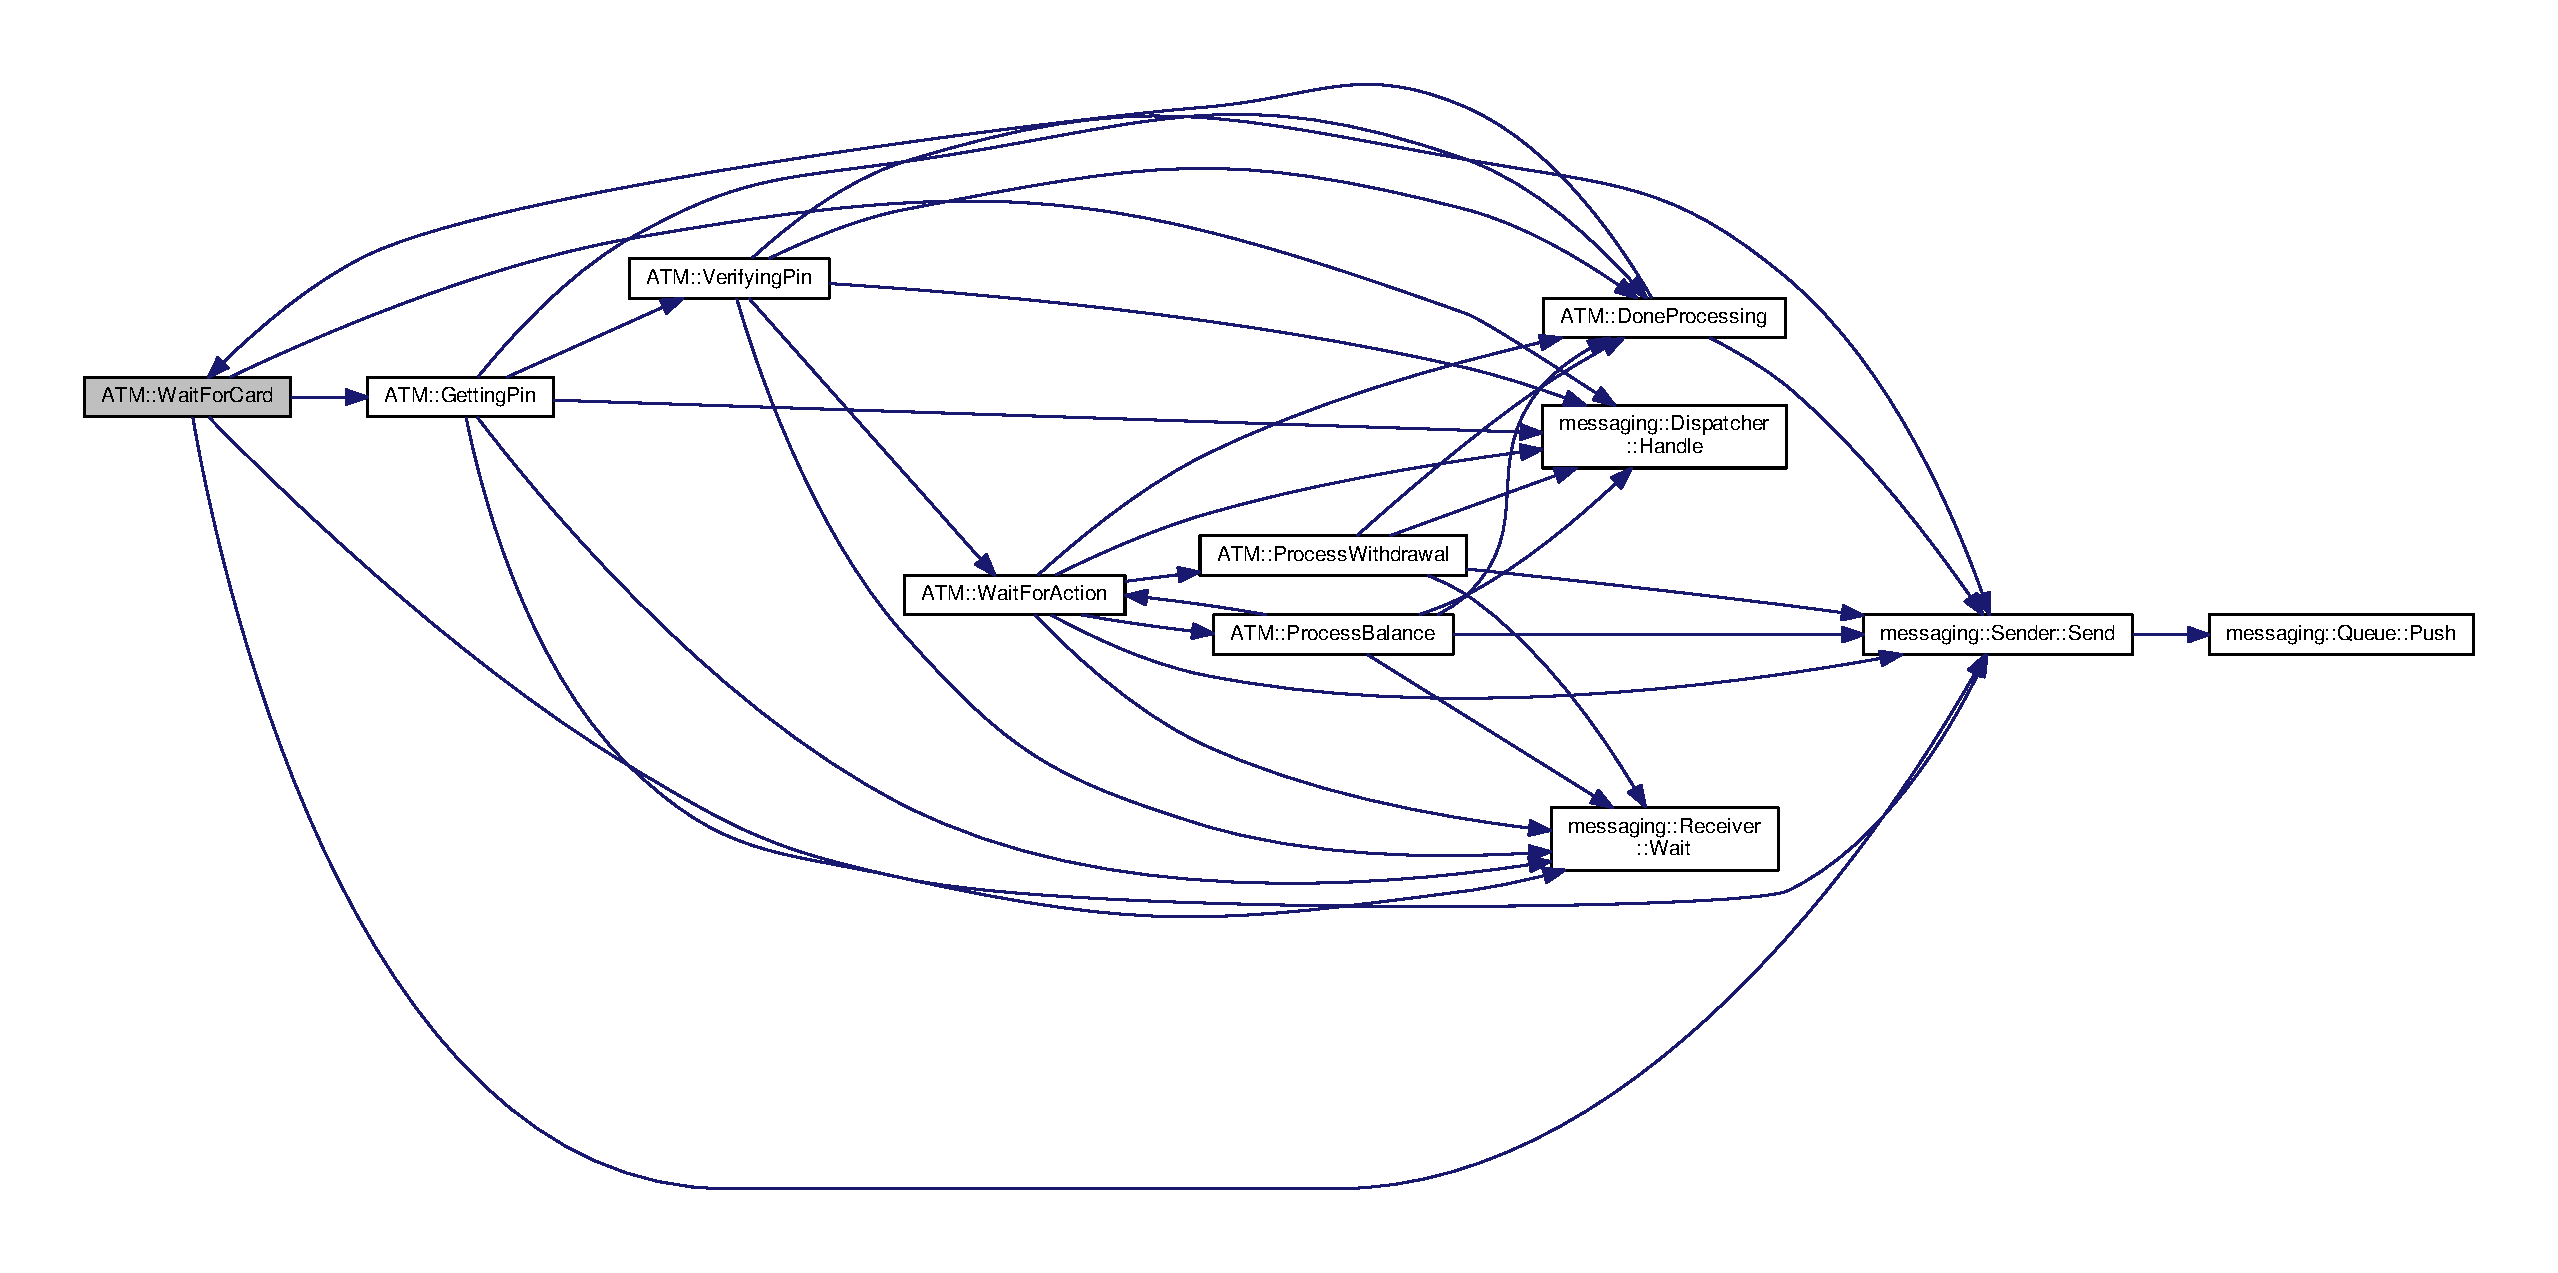
\includegraphics[width=350pt]{classATM_ae530dbaa0e091b13f919542d002ef216_cgraph}
\end{center}
\end{figure}




\subsection{Member Data Documentation}
\hypertarget{classATM_a25cd6fda12c3a95144d820de539adee6}{\index{A\-T\-M@{A\-T\-M}!account\-\_\-@{account\-\_\-}}
\index{account\-\_\-@{account\-\_\-}!ATM@{A\-T\-M}}
\subsubsection[{account\-\_\-}]{\setlength{\rightskip}{0pt plus 5cm}std\-::string A\-T\-M\-::account\-\_\-\hspace{0.3cm}{\ttfamily [private]}}}\label{classATM_a25cd6fda12c3a95144d820de539adee6}
\hypertarget{classATM_ad4f43517a9785b318afb336355672efe}{\index{A\-T\-M@{A\-T\-M}!bank\-\_\-@{bank\-\_\-}}
\index{bank\-\_\-@{bank\-\_\-}!ATM@{A\-T\-M}}
\subsubsection[{bank\-\_\-}]{\setlength{\rightskip}{0pt plus 5cm}{\bf messaging\-::\-Sender} A\-T\-M\-::bank\-\_\-\hspace{0.3cm}{\ttfamily [private]}}}\label{classATM_ad4f43517a9785b318afb336355672efe}
\hypertarget{classATM_a59b7d4c15875982aef0399de08d1c6c0}{\index{A\-T\-M@{A\-T\-M}!incoming\-\_\-@{incoming\-\_\-}}
\index{incoming\-\_\-@{incoming\-\_\-}!ATM@{A\-T\-M}}
\subsubsection[{incoming\-\_\-}]{\setlength{\rightskip}{0pt plus 5cm}{\bf messaging\-::\-Receiver} A\-T\-M\-::incoming\-\_\-\hspace{0.3cm}{\ttfamily [private]}}}\label{classATM_a59b7d4c15875982aef0399de08d1c6c0}
\hypertarget{classATM_aeffb0e1f17d32a7dcf2f84643390e614}{\index{A\-T\-M@{A\-T\-M}!interface\-\_\-hardware\-\_\-@{interface\-\_\-hardware\-\_\-}}
\index{interface\-\_\-hardware\-\_\-@{interface\-\_\-hardware\-\_\-}!ATM@{A\-T\-M}}
\subsubsection[{interface\-\_\-hardware\-\_\-}]{\setlength{\rightskip}{0pt plus 5cm}{\bf messaging\-::\-Sender} A\-T\-M\-::interface\-\_\-hardware\-\_\-\hspace{0.3cm}{\ttfamily [private]}}}\label{classATM_aeffb0e1f17d32a7dcf2f84643390e614}
\hypertarget{classATM_abf1480605c201cac7d94e0057c372517}{\index{A\-T\-M@{A\-T\-M}!pin\-\_\-@{pin\-\_\-}}
\index{pin\-\_\-@{pin\-\_\-}!ATM@{A\-T\-M}}
\subsubsection[{pin\-\_\-}]{\setlength{\rightskip}{0pt plus 5cm}std\-::string A\-T\-M\-::pin\-\_\-\hspace{0.3cm}{\ttfamily [private]}}}\label{classATM_abf1480605c201cac7d94e0057c372517}
\hypertarget{classATM_ad655bcb7436d78fba4b0d16ab9a15ff1}{\index{A\-T\-M@{A\-T\-M}!state\-\_\-@{state\-\_\-}}
\index{state\-\_\-@{state\-\_\-}!ATM@{A\-T\-M}}
\subsubsection[{state\-\_\-}]{\setlength{\rightskip}{0pt plus 5cm}void(A\-T\-M\-::$\ast$ A\-T\-M\-::state\-\_\-)()\hspace{0.3cm}{\ttfamily [private]}}}\label{classATM_ad655bcb7436d78fba4b0d16ab9a15ff1}
\hypertarget{classATM_a45c2bec3b3f822e15db0304d7ed26529}{\index{A\-T\-M@{A\-T\-M}!withdrawal\-\_\-amount\-\_\-@{withdrawal\-\_\-amount\-\_\-}}
\index{withdrawal\-\_\-amount\-\_\-@{withdrawal\-\_\-amount\-\_\-}!ATM@{A\-T\-M}}
\subsubsection[{withdrawal\-\_\-amount\-\_\-}]{\setlength{\rightskip}{0pt plus 5cm}unsigned A\-T\-M\-::withdrawal\-\_\-amount\-\_\-\hspace{0.3cm}{\ttfamily [private]}}}\label{classATM_a45c2bec3b3f822e15db0304d7ed26529}


The documentation for this class was generated from the following file\-:\begin{DoxyCompactItemize}
\item 
/root/\-Public/shack/atm/\hyperlink{atm_8h}{atm.\-h}\end{DoxyCompactItemize}

\hypertarget{structBalance}{\section{Balance Struct Reference}
\label{structBalance}\index{Balance@{Balance}}
}


{\ttfamily \#include $<$withdraw.\-h$>$}

\subsection*{Public Member Functions}
\begin{DoxyCompactItemize}
\item 
\hyperlink{structBalance_a05b22821b169a5764e65c54baa1f6d36}{Balance} (unsigned amount)
\end{DoxyCompactItemize}
\subsection*{Public Attributes}
\begin{DoxyCompactItemize}
\item 
unsigned \hyperlink{structBalance_a5b2f1116c7c0db66012c63527212c042}{amount\-\_\-}
\end{DoxyCompactItemize}


\subsection{Constructor \& Destructor Documentation}
\hypertarget{structBalance_a05b22821b169a5764e65c54baa1f6d36}{\index{Balance@{Balance}!Balance@{Balance}}
\index{Balance@{Balance}!Balance@{Balance}}
\subsubsection[{Balance}]{\setlength{\rightskip}{0pt plus 5cm}Balance\-::\-Balance (
\begin{DoxyParamCaption}
\item[{unsigned}]{amount}
\end{DoxyParamCaption}
)\hspace{0.3cm}{\ttfamily [inline]}, {\ttfamily [explicit]}}}\label{structBalance_a05b22821b169a5764e65c54baa1f6d36}


\subsection{Member Data Documentation}
\hypertarget{structBalance_a5b2f1116c7c0db66012c63527212c042}{\index{Balance@{Balance}!amount\-\_\-@{amount\-\_\-}}
\index{amount\-\_\-@{amount\-\_\-}!Balance@{Balance}}
\subsubsection[{amount\-\_\-}]{\setlength{\rightskip}{0pt plus 5cm}unsigned Balance\-::amount\-\_\-}}\label{structBalance_a5b2f1116c7c0db66012c63527212c042}


The documentation for this struct was generated from the following file\-:\begin{DoxyCompactItemize}
\item 
/root/\-Public/shack/atm/\hyperlink{withdraw_8h}{withdraw.\-h}\end{DoxyCompactItemize}

\hypertarget{structBalancePressed}{\section{Balance\-Pressed Struct Reference}
\label{structBalancePressed}\index{Balance\-Pressed@{Balance\-Pressed}}
}


{\ttfamily \#include $<$withdraw.\-h$>$}



The documentation for this struct was generated from the following file\-:\begin{DoxyCompactItemize}
\item 
/root/\-Public/shack/atm/\hyperlink{withdraw_8h}{withdraw.\-h}\end{DoxyCompactItemize}

\hypertarget{classBankMachine}{\section{Bank\-Machine Class Reference}
\label{classBankMachine}\index{Bank\-Machine@{Bank\-Machine}}
}


{\ttfamily \#include $<$bank\-\_\-machine.\-h$>$}



Collaboration diagram for Bank\-Machine\-:
\nopagebreak
\begin{figure}[H]
\begin{center}
\leavevmode
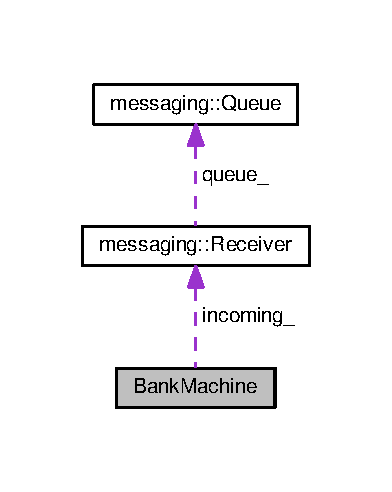
\includegraphics[width=188pt]{classBankMachine__coll__graph}
\end{center}
\end{figure}
\subsection*{Public Member Functions}
\begin{DoxyCompactItemize}
\item 
\hyperlink{classBankMachine_aafdb9bf4f04bec9c6ac3b9ec2229843e}{Bank\-Machine} ()
\item 
void \hyperlink{classBankMachine_afaf799b68e5965bb473cee993fffee74}{Done} ()
\item 
void \hyperlink{classBankMachine_adba1d635c9837305c1e0fe4f70efdcdb}{Run} ()
\item 
\hyperlink{classmessaging_1_1Sender}{messaging\-::\-Sender} \hyperlink{classBankMachine_a5d8bf0c5b153073a6bfa76bd2ee29acb}{Get\-Sender} ()
\end{DoxyCompactItemize}
\subsection*{Private Attributes}
\begin{DoxyCompactItemize}
\item 
\hyperlink{classmessaging_1_1Receiver}{messaging\-::\-Receiver} \hyperlink{classBankMachine_a80fe063f235cf02d33a2d70aeef6048c}{incoming\-\_\-}
\item 
unsigned \hyperlink{classBankMachine_ad299fdb18b1ee6e66374f70dde18d584}{balance\-\_\-}
\end{DoxyCompactItemize}


\subsection{Constructor \& Destructor Documentation}
\hypertarget{classBankMachine_aafdb9bf4f04bec9c6ac3b9ec2229843e}{\index{Bank\-Machine@{Bank\-Machine}!Bank\-Machine@{Bank\-Machine}}
\index{Bank\-Machine@{Bank\-Machine}!BankMachine@{Bank\-Machine}}
\subsubsection[{Bank\-Machine}]{\setlength{\rightskip}{0pt plus 5cm}Bank\-Machine\-::\-Bank\-Machine (
\begin{DoxyParamCaption}
{}
\end{DoxyParamCaption}
)\hspace{0.3cm}{\ttfamily [inline]}}}\label{classBankMachine_aafdb9bf4f04bec9c6ac3b9ec2229843e}


\subsection{Member Function Documentation}
\hypertarget{classBankMachine_afaf799b68e5965bb473cee993fffee74}{\index{Bank\-Machine@{Bank\-Machine}!Done@{Done}}
\index{Done@{Done}!BankMachine@{Bank\-Machine}}
\subsubsection[{Done}]{\setlength{\rightskip}{0pt plus 5cm}void Bank\-Machine\-::\-Done (
\begin{DoxyParamCaption}
{}
\end{DoxyParamCaption}
)\hspace{0.3cm}{\ttfamily [inline]}}}\label{classBankMachine_afaf799b68e5965bb473cee993fffee74}


Here is the call graph for this function\-:\nopagebreak
\begin{figure}[H]
\begin{center}
\leavevmode
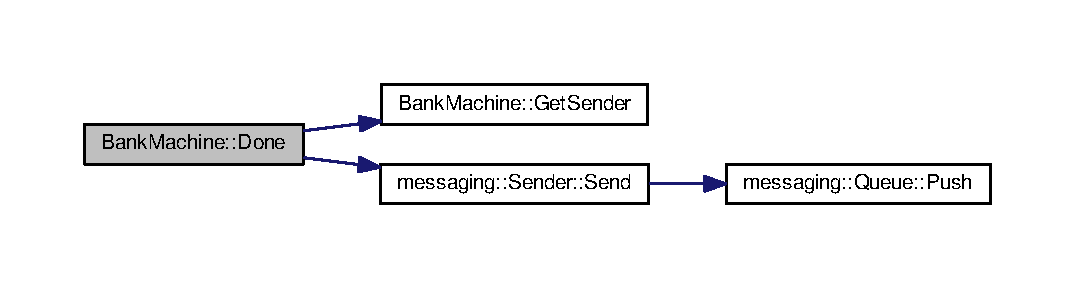
\includegraphics[width=350pt]{classBankMachine_afaf799b68e5965bb473cee993fffee74_cgraph}
\end{center}
\end{figure}


\hypertarget{classBankMachine_a5d8bf0c5b153073a6bfa76bd2ee29acb}{\index{Bank\-Machine@{Bank\-Machine}!Get\-Sender@{Get\-Sender}}
\index{Get\-Sender@{Get\-Sender}!BankMachine@{Bank\-Machine}}
\subsubsection[{Get\-Sender}]{\setlength{\rightskip}{0pt plus 5cm}{\bf messaging\-::\-Sender} Bank\-Machine\-::\-Get\-Sender (
\begin{DoxyParamCaption}
{}
\end{DoxyParamCaption}
)\hspace{0.3cm}{\ttfamily [inline]}}}\label{classBankMachine_a5d8bf0c5b153073a6bfa76bd2ee29acb}
\hypertarget{classBankMachine_adba1d635c9837305c1e0fe4f70efdcdb}{\index{Bank\-Machine@{Bank\-Machine}!Run@{Run}}
\index{Run@{Run}!BankMachine@{Bank\-Machine}}
\subsubsection[{Run}]{\setlength{\rightskip}{0pt plus 5cm}void Bank\-Machine\-::\-Run (
\begin{DoxyParamCaption}
{}
\end{DoxyParamCaption}
)\hspace{0.3cm}{\ttfamily [inline]}}}\label{classBankMachine_adba1d635c9837305c1e0fe4f70efdcdb}


Here is the call graph for this function\-:\nopagebreak
\begin{figure}[H]
\begin{center}
\leavevmode
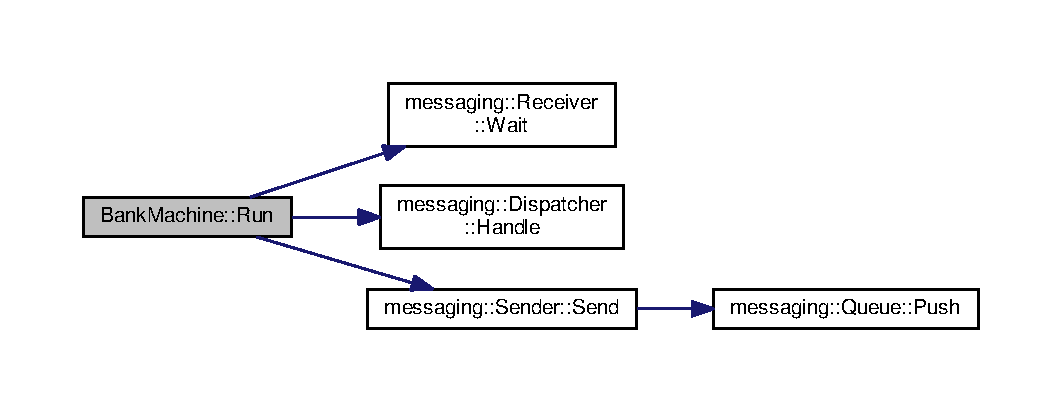
\includegraphics[width=350pt]{classBankMachine_adba1d635c9837305c1e0fe4f70efdcdb_cgraph}
\end{center}
\end{figure}




\subsection{Member Data Documentation}
\hypertarget{classBankMachine_ad299fdb18b1ee6e66374f70dde18d584}{\index{Bank\-Machine@{Bank\-Machine}!balance\-\_\-@{balance\-\_\-}}
\index{balance\-\_\-@{balance\-\_\-}!BankMachine@{Bank\-Machine}}
\subsubsection[{balance\-\_\-}]{\setlength{\rightskip}{0pt plus 5cm}unsigned Bank\-Machine\-::balance\-\_\-\hspace{0.3cm}{\ttfamily [private]}}}\label{classBankMachine_ad299fdb18b1ee6e66374f70dde18d584}
\hypertarget{classBankMachine_a80fe063f235cf02d33a2d70aeef6048c}{\index{Bank\-Machine@{Bank\-Machine}!incoming\-\_\-@{incoming\-\_\-}}
\index{incoming\-\_\-@{incoming\-\_\-}!BankMachine@{Bank\-Machine}}
\subsubsection[{incoming\-\_\-}]{\setlength{\rightskip}{0pt plus 5cm}{\bf messaging\-::\-Receiver} Bank\-Machine\-::incoming\-\_\-\hspace{0.3cm}{\ttfamily [private]}}}\label{classBankMachine_a80fe063f235cf02d33a2d70aeef6048c}


The documentation for this class was generated from the following file\-:\begin{DoxyCompactItemize}
\item 
/root/\-Public/shack/atm/\hyperlink{bank__machine_8h}{bank\-\_\-machine.\-h}\end{DoxyCompactItemize}

\hypertarget{structCancelPressed}{\section{Cancel\-Pressed Struct Reference}
\label{structCancelPressed}\index{Cancel\-Pressed@{Cancel\-Pressed}}
}


{\ttfamily \#include $<$withdraw.\-h$>$}



The documentation for this struct was generated from the following file\-:\begin{DoxyCompactItemize}
\item 
/root/\-Public/shack/atm/\hyperlink{withdraw_8h}{withdraw.\-h}\end{DoxyCompactItemize}

\hypertarget{structCancelWithdrawal}{\section{Cancel\-Withdrawal Struct Reference}
\label{structCancelWithdrawal}\index{Cancel\-Withdrawal@{Cancel\-Withdrawal}}
}


{\ttfamily \#include $<$withdraw.\-h$>$}

\subsection*{Public Member Functions}
\begin{DoxyCompactItemize}
\item 
\hyperlink{structCancelWithdrawal_a57f5a52f8b47152f11e9cef892326c1e}{Cancel\-Withdrawal} (const std\-::string \&account, unsigned amount)
\end{DoxyCompactItemize}
\subsection*{Public Attributes}
\begin{DoxyCompactItemize}
\item 
std\-::string \hyperlink{structCancelWithdrawal_a4a081ab8be5299d5032139dbe774603f}{account\-\_\-}
\item 
unsigned \hyperlink{structCancelWithdrawal_a27d03ed0ebc0fbd59b82076431782bcf}{amount\-\_\-}
\end{DoxyCompactItemize}


\subsection{Constructor \& Destructor Documentation}
\hypertarget{structCancelWithdrawal_a57f5a52f8b47152f11e9cef892326c1e}{\index{Cancel\-Withdrawal@{Cancel\-Withdrawal}!Cancel\-Withdrawal@{Cancel\-Withdrawal}}
\index{Cancel\-Withdrawal@{Cancel\-Withdrawal}!CancelWithdrawal@{Cancel\-Withdrawal}}
\subsubsection[{Cancel\-Withdrawal}]{\setlength{\rightskip}{0pt plus 5cm}Cancel\-Withdrawal\-::\-Cancel\-Withdrawal (
\begin{DoxyParamCaption}
\item[{const std\-::string \&}]{account, }
\item[{unsigned}]{amount}
\end{DoxyParamCaption}
)\hspace{0.3cm}{\ttfamily [inline]}}}\label{structCancelWithdrawal_a57f5a52f8b47152f11e9cef892326c1e}


\subsection{Member Data Documentation}
\hypertarget{structCancelWithdrawal_a4a081ab8be5299d5032139dbe774603f}{\index{Cancel\-Withdrawal@{Cancel\-Withdrawal}!account\-\_\-@{account\-\_\-}}
\index{account\-\_\-@{account\-\_\-}!CancelWithdrawal@{Cancel\-Withdrawal}}
\subsubsection[{account\-\_\-}]{\setlength{\rightskip}{0pt plus 5cm}std\-::string Cancel\-Withdrawal\-::account\-\_\-}}\label{structCancelWithdrawal_a4a081ab8be5299d5032139dbe774603f}
\hypertarget{structCancelWithdrawal_a27d03ed0ebc0fbd59b82076431782bcf}{\index{Cancel\-Withdrawal@{Cancel\-Withdrawal}!amount\-\_\-@{amount\-\_\-}}
\index{amount\-\_\-@{amount\-\_\-}!CancelWithdrawal@{Cancel\-Withdrawal}}
\subsubsection[{amount\-\_\-}]{\setlength{\rightskip}{0pt plus 5cm}unsigned Cancel\-Withdrawal\-::amount\-\_\-}}\label{structCancelWithdrawal_a27d03ed0ebc0fbd59b82076431782bcf}


The documentation for this struct was generated from the following file\-:\begin{DoxyCompactItemize}
\item 
/root/\-Public/shack/atm/\hyperlink{withdraw_8h}{withdraw.\-h}\end{DoxyCompactItemize}

\hypertarget{structCardInserted}{\section{Card\-Inserted Struct Reference}
\label{structCardInserted}\index{Card\-Inserted@{Card\-Inserted}}
}


{\ttfamily \#include $<$withdraw.\-h$>$}

\subsection*{Public Member Functions}
\begin{DoxyCompactItemize}
\item 
\hyperlink{structCardInserted_ae0b0ec1c6170fd1ac7ccfb54fb8116c8}{Card\-Inserted} (const std\-::string account)
\end{DoxyCompactItemize}
\subsection*{Public Attributes}
\begin{DoxyCompactItemize}
\item 
std\-::string \hyperlink{structCardInserted_a9505cd0aa6f6faa1ef3a6203babfa5f9}{account\-\_\-}
\end{DoxyCompactItemize}


\subsection{Constructor \& Destructor Documentation}
\hypertarget{structCardInserted_ae0b0ec1c6170fd1ac7ccfb54fb8116c8}{\index{Card\-Inserted@{Card\-Inserted}!Card\-Inserted@{Card\-Inserted}}
\index{Card\-Inserted@{Card\-Inserted}!CardInserted@{Card\-Inserted}}
\subsubsection[{Card\-Inserted}]{\setlength{\rightskip}{0pt plus 5cm}Card\-Inserted\-::\-Card\-Inserted (
\begin{DoxyParamCaption}
\item[{const std\-::string}]{account}
\end{DoxyParamCaption}
)\hspace{0.3cm}{\ttfamily [inline]}, {\ttfamily [explicit]}}}\label{structCardInserted_ae0b0ec1c6170fd1ac7ccfb54fb8116c8}


\subsection{Member Data Documentation}
\hypertarget{structCardInserted_a9505cd0aa6f6faa1ef3a6203babfa5f9}{\index{Card\-Inserted@{Card\-Inserted}!account\-\_\-@{account\-\_\-}}
\index{account\-\_\-@{account\-\_\-}!CardInserted@{Card\-Inserted}}
\subsubsection[{account\-\_\-}]{\setlength{\rightskip}{0pt plus 5cm}std\-::string Card\-Inserted\-::account\-\_\-}}\label{structCardInserted_a9505cd0aa6f6faa1ef3a6203babfa5f9}


The documentation for this struct was generated from the following file\-:\begin{DoxyCompactItemize}
\item 
/root/\-Public/shack/atm/\hyperlink{withdraw_8h}{withdraw.\-h}\end{DoxyCompactItemize}

\hypertarget{structClearLastPressed}{\section{Clear\-Last\-Pressed Struct Reference}
\label{structClearLastPressed}\index{Clear\-Last\-Pressed@{Clear\-Last\-Pressed}}
}


{\ttfamily \#include $<$withdraw.\-h$>$}



The documentation for this struct was generated from the following file\-:\begin{DoxyCompactItemize}
\item 
/root/\-Public/shack/atm/\hyperlink{withdraw_8h}{withdraw.\-h}\end{DoxyCompactItemize}

\hypertarget{classmessaging_1_1CloseQueue}{\section{messaging\-:\-:Close\-Queue Class Reference}
\label{classmessaging_1_1CloseQueue}\index{messaging\-::\-Close\-Queue@{messaging\-::\-Close\-Queue}}
}


{\ttfamily \#include $<$dispatcher.\-h$>$}



The documentation for this class was generated from the following file\-:\begin{DoxyCompactItemize}
\item 
/root/\-Public/shack/atm/\hyperlink{dispatcher_8h}{dispatcher.\-h}\end{DoxyCompactItemize}

\hypertarget{structDigitPressed}{\section{Digit\-Pressed Struct Reference}
\label{structDigitPressed}\index{Digit\-Pressed@{Digit\-Pressed}}
}


{\ttfamily \#include $<$withdraw.\-h$>$}

\subsection*{Public Member Functions}
\begin{DoxyCompactItemize}
\item 
\hyperlink{structDigitPressed_ac18455a16841020dce7f7eb52950bad8}{Digit\-Pressed} (char digit)
\end{DoxyCompactItemize}
\subsection*{Public Attributes}
\begin{DoxyCompactItemize}
\item 
char \hyperlink{structDigitPressed_a4df37896f8d63954fc5673c9ff571317}{digit\-\_\-}
\end{DoxyCompactItemize}


\subsection{Constructor \& Destructor Documentation}
\hypertarget{structDigitPressed_ac18455a16841020dce7f7eb52950bad8}{\index{Digit\-Pressed@{Digit\-Pressed}!Digit\-Pressed@{Digit\-Pressed}}
\index{Digit\-Pressed@{Digit\-Pressed}!DigitPressed@{Digit\-Pressed}}
\subsubsection[{Digit\-Pressed}]{\setlength{\rightskip}{0pt plus 5cm}Digit\-Pressed\-::\-Digit\-Pressed (
\begin{DoxyParamCaption}
\item[{char}]{digit}
\end{DoxyParamCaption}
)\hspace{0.3cm}{\ttfamily [inline]}, {\ttfamily [explicit]}}}\label{structDigitPressed_ac18455a16841020dce7f7eb52950bad8}


\subsection{Member Data Documentation}
\hypertarget{structDigitPressed_a4df37896f8d63954fc5673c9ff571317}{\index{Digit\-Pressed@{Digit\-Pressed}!digit\-\_\-@{digit\-\_\-}}
\index{digit\-\_\-@{digit\-\_\-}!DigitPressed@{Digit\-Pressed}}
\subsubsection[{digit\-\_\-}]{\setlength{\rightskip}{0pt plus 5cm}char Digit\-Pressed\-::digit\-\_\-}}\label{structDigitPressed_a4df37896f8d63954fc5673c9ff571317}


The documentation for this struct was generated from the following file\-:\begin{DoxyCompactItemize}
\item 
/root/\-Public/shack/atm/\hyperlink{withdraw_8h}{withdraw.\-h}\end{DoxyCompactItemize}

\hypertarget{classmessaging_1_1Dispatcher}{\section{messaging\-:\-:Dispatcher Class Reference}
\label{classmessaging_1_1Dispatcher}\index{messaging\-::\-Dispatcher@{messaging\-::\-Dispatcher}}
}


{\ttfamily \#include $<$dispatcher.\-h$>$}



Collaboration diagram for messaging\-:\-:Dispatcher\-:
\nopagebreak
\begin{figure}[H]
\begin{center}
\leavevmode
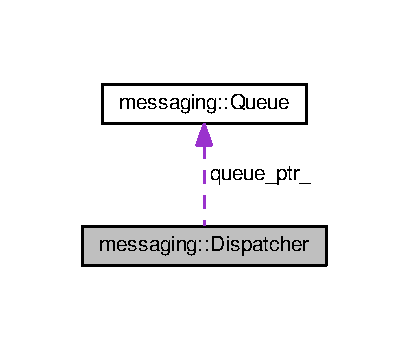
\includegraphics[width=196pt]{classmessaging_1_1Dispatcher__coll__graph}
\end{center}
\end{figure}
\subsection*{Public Member Functions}
\begin{DoxyCompactItemize}
\item 
\hyperlink{classmessaging_1_1Dispatcher_a80bdf7cb7e206ccb6709a74b1d015682}{Dispatcher} (\hyperlink{classmessaging_1_1Dispatcher}{Dispatcher} \&\&other)
\item 
\hyperlink{classmessaging_1_1Dispatcher_adb867c8b876c901d12154e12406e8ff8}{Dispatcher} (\hyperlink{classmessaging_1_1Queue}{Queue} $\ast$queue)
\item 
{\footnotesize template$<$class Message , class Func $>$ }\\\hyperlink{classmessaging_1_1TemplateDispatcher}{Template\-Dispatcher}$<$ \hyperlink{classmessaging_1_1Dispatcher}{Dispatcher}, \\*
Message, Func $>$ \hyperlink{classmessaging_1_1Dispatcher_a6d9d0bf1da266ca951c7821bc4e84f9f}{Handle} (Func \&\&f)
\item 
\hyperlink{classmessaging_1_1Dispatcher_ac17a4675e9a484de43bdf8914ab93d04}{$\sim$\-Dispatcher} () noexcept(false)
\end{DoxyCompactItemize}
\subsection*{Private Member Functions}
\begin{DoxyCompactItemize}
\item 
\hyperlink{classmessaging_1_1Dispatcher_a6b50ba4fc04d8971bc9ddb3934c8134a}{Dispatcher} (const \hyperlink{classmessaging_1_1Dispatcher}{Dispatcher} \&)=delete
\item 
\hyperlink{classmessaging_1_1Dispatcher}{Dispatcher} \& \hyperlink{classmessaging_1_1Dispatcher_a633a26a5b07d92045164800ba86c01e2}{operator=} (const \hyperlink{classmessaging_1_1Dispatcher}{Dispatcher} \&)=delete
\item 
void \hyperlink{classmessaging_1_1Dispatcher_a0318b520773a5c7a144fa8b9e8a0dd61}{Wait\-And\-Dispatch} ()
\item 
bool \hyperlink{classmessaging_1_1Dispatcher_a4fe4a8aa09f0f97676eef973cceb0ef5}{Dispatch} (const std\-::shared\-\_\-ptr$<$ \hyperlink{structmessaging_1_1MessageBase}{Message\-Base} $>$ \&msg)
\end{DoxyCompactItemize}
\subsection*{Private Attributes}
\begin{DoxyCompactItemize}
\item 
\hyperlink{classmessaging_1_1Queue}{Queue} $\ast$ \hyperlink{classmessaging_1_1Dispatcher_a877e071792b0e42b46c7d32836de0739}{queue\-\_\-ptr\-\_\-}
\item 
bool \hyperlink{classmessaging_1_1Dispatcher_a4db2da2c17f91e2c9b119b60fe4fee0a}{chained\-\_\-}
\end{DoxyCompactItemize}
\subsection*{Friends}
\begin{DoxyCompactItemize}
\item 
{\footnotesize template$<$class Dispatcher , class Msg , class Func $>$ }\\class \hyperlink{classmessaging_1_1Dispatcher_ac52eebabf93ac84bc8eacc5c67e6ca9f}{Template\-Dispatcher}
\end{DoxyCompactItemize}


\subsection{Constructor \& Destructor Documentation}
\hypertarget{classmessaging_1_1Dispatcher_a80bdf7cb7e206ccb6709a74b1d015682}{\index{messaging\-::\-Dispatcher@{messaging\-::\-Dispatcher}!Dispatcher@{Dispatcher}}
\index{Dispatcher@{Dispatcher}!messaging::Dispatcher@{messaging\-::\-Dispatcher}}
\subsubsection[{Dispatcher}]{\setlength{\rightskip}{0pt plus 5cm}messaging\-::\-Dispatcher\-::\-Dispatcher (
\begin{DoxyParamCaption}
\item[{{\bf Dispatcher} \&\&}]{other}
\end{DoxyParamCaption}
)\hspace{0.3cm}{\ttfamily [inline]}}}\label{classmessaging_1_1Dispatcher_a80bdf7cb7e206ccb6709a74b1d015682}
\hypertarget{classmessaging_1_1Dispatcher_adb867c8b876c901d12154e12406e8ff8}{\index{messaging\-::\-Dispatcher@{messaging\-::\-Dispatcher}!Dispatcher@{Dispatcher}}
\index{Dispatcher@{Dispatcher}!messaging::Dispatcher@{messaging\-::\-Dispatcher}}
\subsubsection[{Dispatcher}]{\setlength{\rightskip}{0pt plus 5cm}messaging\-::\-Dispatcher\-::\-Dispatcher (
\begin{DoxyParamCaption}
\item[{{\bf Queue} $\ast$}]{queue}
\end{DoxyParamCaption}
)\hspace{0.3cm}{\ttfamily [inline]}, {\ttfamily [explicit]}}}\label{classmessaging_1_1Dispatcher_adb867c8b876c901d12154e12406e8ff8}
\hypertarget{classmessaging_1_1Dispatcher_ac17a4675e9a484de43bdf8914ab93d04}{\index{messaging\-::\-Dispatcher@{messaging\-::\-Dispatcher}!$\sim$\-Dispatcher@{$\sim$\-Dispatcher}}
\index{$\sim$\-Dispatcher@{$\sim$\-Dispatcher}!messaging::Dispatcher@{messaging\-::\-Dispatcher}}
\subsubsection[{$\sim$\-Dispatcher}]{\setlength{\rightskip}{0pt plus 5cm}messaging\-::\-Dispatcher\-::$\sim$\-Dispatcher (
\begin{DoxyParamCaption}
{}
\end{DoxyParamCaption}
)\hspace{0.3cm}{\ttfamily [inline]}, {\ttfamily [noexcept]}}}\label{classmessaging_1_1Dispatcher_ac17a4675e9a484de43bdf8914ab93d04}


Here is the call graph for this function\-:
\nopagebreak
\begin{figure}[H]
\begin{center}
\leavevmode
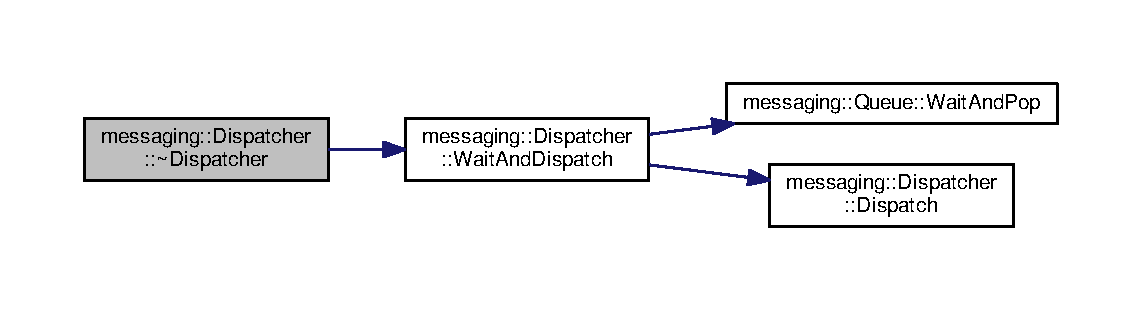
\includegraphics[width=350pt]{classmessaging_1_1Dispatcher_ac17a4675e9a484de43bdf8914ab93d04_cgraph}
\end{center}
\end{figure}


\hypertarget{classmessaging_1_1Dispatcher_a6b50ba4fc04d8971bc9ddb3934c8134a}{\index{messaging\-::\-Dispatcher@{messaging\-::\-Dispatcher}!Dispatcher@{Dispatcher}}
\index{Dispatcher@{Dispatcher}!messaging::Dispatcher@{messaging\-::\-Dispatcher}}
\subsubsection[{Dispatcher}]{\setlength{\rightskip}{0pt plus 5cm}messaging\-::\-Dispatcher\-::\-Dispatcher (
\begin{DoxyParamCaption}
\item[{const {\bf Dispatcher} \&}]{}
\end{DoxyParamCaption}
)\hspace{0.3cm}{\ttfamily [private]}, {\ttfamily [delete]}}}\label{classmessaging_1_1Dispatcher_a6b50ba4fc04d8971bc9ddb3934c8134a}


\subsection{Member Function Documentation}
\hypertarget{classmessaging_1_1Dispatcher_a4fe4a8aa09f0f97676eef973cceb0ef5}{\index{messaging\-::\-Dispatcher@{messaging\-::\-Dispatcher}!Dispatch@{Dispatch}}
\index{Dispatch@{Dispatch}!messaging::Dispatcher@{messaging\-::\-Dispatcher}}
\subsubsection[{Dispatch}]{\setlength{\rightskip}{0pt plus 5cm}bool messaging\-::\-Dispatcher\-::\-Dispatch (
\begin{DoxyParamCaption}
\item[{const std\-::shared\-\_\-ptr$<$ {\bf Message\-Base} $>$ \&}]{msg}
\end{DoxyParamCaption}
)\hspace{0.3cm}{\ttfamily [inline]}, {\ttfamily [private]}}}\label{classmessaging_1_1Dispatcher_a4fe4a8aa09f0f97676eef973cceb0ef5}
\hypertarget{classmessaging_1_1Dispatcher_a6d9d0bf1da266ca951c7821bc4e84f9f}{\index{messaging\-::\-Dispatcher@{messaging\-::\-Dispatcher}!Handle@{Handle}}
\index{Handle@{Handle}!messaging::Dispatcher@{messaging\-::\-Dispatcher}}
\subsubsection[{Handle}]{\setlength{\rightskip}{0pt plus 5cm}template$<$class Message , class Func $>$ {\bf Template\-Dispatcher}$<${\bf Dispatcher}, Message, Func$>$ messaging\-::\-Dispatcher\-::\-Handle (
\begin{DoxyParamCaption}
\item[{Func \&\&}]{f}
\end{DoxyParamCaption}
)\hspace{0.3cm}{\ttfamily [inline]}}}\label{classmessaging_1_1Dispatcher_a6d9d0bf1da266ca951c7821bc4e84f9f}
\hypertarget{classmessaging_1_1Dispatcher_a633a26a5b07d92045164800ba86c01e2}{\index{messaging\-::\-Dispatcher@{messaging\-::\-Dispatcher}!operator=@{operator=}}
\index{operator=@{operator=}!messaging::Dispatcher@{messaging\-::\-Dispatcher}}
\subsubsection[{operator=}]{\setlength{\rightskip}{0pt plus 5cm}{\bf Dispatcher}\& messaging\-::\-Dispatcher\-::operator= (
\begin{DoxyParamCaption}
\item[{const {\bf Dispatcher} \&}]{}
\end{DoxyParamCaption}
)\hspace{0.3cm}{\ttfamily [private]}, {\ttfamily [delete]}}}\label{classmessaging_1_1Dispatcher_a633a26a5b07d92045164800ba86c01e2}
\hypertarget{classmessaging_1_1Dispatcher_a0318b520773a5c7a144fa8b9e8a0dd61}{\index{messaging\-::\-Dispatcher@{messaging\-::\-Dispatcher}!Wait\-And\-Dispatch@{Wait\-And\-Dispatch}}
\index{Wait\-And\-Dispatch@{Wait\-And\-Dispatch}!messaging::Dispatcher@{messaging\-::\-Dispatcher}}
\subsubsection[{Wait\-And\-Dispatch}]{\setlength{\rightskip}{0pt plus 5cm}void messaging\-::\-Dispatcher\-::\-Wait\-And\-Dispatch (
\begin{DoxyParamCaption}
{}
\end{DoxyParamCaption}
)\hspace{0.3cm}{\ttfamily [inline]}, {\ttfamily [private]}}}\label{classmessaging_1_1Dispatcher_a0318b520773a5c7a144fa8b9e8a0dd61}


Here is the call graph for this function\-:
\nopagebreak
\begin{figure}[H]
\begin{center}
\leavevmode
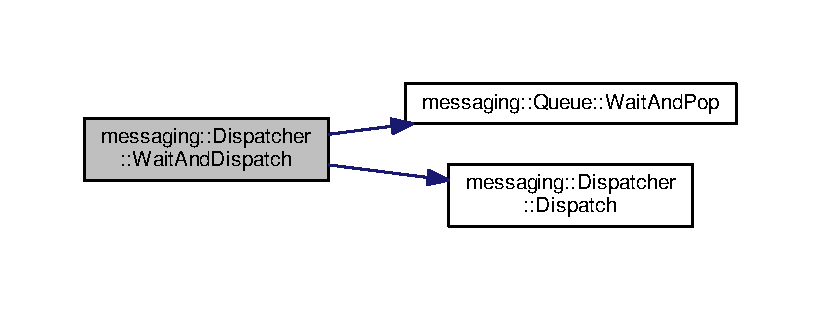
\includegraphics[width=350pt]{classmessaging_1_1Dispatcher_a0318b520773a5c7a144fa8b9e8a0dd61_cgraph}
\end{center}
\end{figure}




\subsection{Friends And Related Function Documentation}
\hypertarget{classmessaging_1_1Dispatcher_ac52eebabf93ac84bc8eacc5c67e6ca9f}{\index{messaging\-::\-Dispatcher@{messaging\-::\-Dispatcher}!Template\-Dispatcher@{Template\-Dispatcher}}
\index{Template\-Dispatcher@{Template\-Dispatcher}!messaging::Dispatcher@{messaging\-::\-Dispatcher}}
\subsubsection[{Template\-Dispatcher}]{\setlength{\rightskip}{0pt plus 5cm}template$<$class Dispatcher , class Msg , class Func $>$ friend class {\bf Template\-Dispatcher}\hspace{0.3cm}{\ttfamily [friend]}}}\label{classmessaging_1_1Dispatcher_ac52eebabf93ac84bc8eacc5c67e6ca9f}


\subsection{Member Data Documentation}
\hypertarget{classmessaging_1_1Dispatcher_a4db2da2c17f91e2c9b119b60fe4fee0a}{\index{messaging\-::\-Dispatcher@{messaging\-::\-Dispatcher}!chained\-\_\-@{chained\-\_\-}}
\index{chained\-\_\-@{chained\-\_\-}!messaging::Dispatcher@{messaging\-::\-Dispatcher}}
\subsubsection[{chained\-\_\-}]{\setlength{\rightskip}{0pt plus 5cm}bool messaging\-::\-Dispatcher\-::chained\-\_\-\hspace{0.3cm}{\ttfamily [private]}}}\label{classmessaging_1_1Dispatcher_a4db2da2c17f91e2c9b119b60fe4fee0a}
\hypertarget{classmessaging_1_1Dispatcher_a877e071792b0e42b46c7d32836de0739}{\index{messaging\-::\-Dispatcher@{messaging\-::\-Dispatcher}!queue\-\_\-ptr\-\_\-@{queue\-\_\-ptr\-\_\-}}
\index{queue\-\_\-ptr\-\_\-@{queue\-\_\-ptr\-\_\-}!messaging::Dispatcher@{messaging\-::\-Dispatcher}}
\subsubsection[{queue\-\_\-ptr\-\_\-}]{\setlength{\rightskip}{0pt plus 5cm}{\bf Queue}$\ast$ messaging\-::\-Dispatcher\-::queue\-\_\-ptr\-\_\-\hspace{0.3cm}{\ttfamily [private]}}}\label{classmessaging_1_1Dispatcher_a877e071792b0e42b46c7d32836de0739}


The documentation for this class was generated from the following file\-:\begin{DoxyCompactItemize}
\item 
/root/\-Public/shack/atm/\hyperlink{dispatcher_8h}{dispatcher.\-h}\end{DoxyCompactItemize}

\hypertarget{structDisplayBalance}{\section{Display\-Balance Struct Reference}
\label{structDisplayBalance}\index{Display\-Balance@{Display\-Balance}}
}


{\ttfamily \#include $<$withdraw.\-h$>$}

\subsection*{Public Member Functions}
\begin{DoxyCompactItemize}
\item 
\hyperlink{structDisplayBalance_a4795f3b85f330fa5474e14acc8c28926}{Display\-Balance} (unsigned amount)
\end{DoxyCompactItemize}
\subsection*{Public Attributes}
\begin{DoxyCompactItemize}
\item 
unsigned \hyperlink{structDisplayBalance_ac6c41137f614b04130e57c4ca574cc7c}{amount\-\_\-}
\end{DoxyCompactItemize}


\subsection{Constructor \& Destructor Documentation}
\hypertarget{structDisplayBalance_a4795f3b85f330fa5474e14acc8c28926}{\index{Display\-Balance@{Display\-Balance}!Display\-Balance@{Display\-Balance}}
\index{Display\-Balance@{Display\-Balance}!DisplayBalance@{Display\-Balance}}
\subsubsection[{Display\-Balance}]{\setlength{\rightskip}{0pt plus 5cm}Display\-Balance\-::\-Display\-Balance (
\begin{DoxyParamCaption}
\item[{unsigned}]{amount}
\end{DoxyParamCaption}
)\hspace{0.3cm}{\ttfamily [inline]}, {\ttfamily [explicit]}}}\label{structDisplayBalance_a4795f3b85f330fa5474e14acc8c28926}


\subsection{Member Data Documentation}
\hypertarget{structDisplayBalance_ac6c41137f614b04130e57c4ca574cc7c}{\index{Display\-Balance@{Display\-Balance}!amount\-\_\-@{amount\-\_\-}}
\index{amount\-\_\-@{amount\-\_\-}!DisplayBalance@{Display\-Balance}}
\subsubsection[{amount\-\_\-}]{\setlength{\rightskip}{0pt plus 5cm}unsigned Display\-Balance\-::amount\-\_\-}}\label{structDisplayBalance_ac6c41137f614b04130e57c4ca574cc7c}


The documentation for this struct was generated from the following file\-:\begin{DoxyCompactItemize}
\item 
/root/\-Public/shack/atm/\hyperlink{withdraw_8h}{withdraw.\-h}\end{DoxyCompactItemize}

\hypertarget{structDisplayEnterCard}{\section{Display\-Enter\-Card Struct Reference}
\label{structDisplayEnterCard}\index{Display\-Enter\-Card@{Display\-Enter\-Card}}
}


{\ttfamily \#include $<$withdraw.\-h$>$}



The documentation for this struct was generated from the following file\-:\begin{DoxyCompactItemize}
\item 
/root/\-Public/shack/atm/\hyperlink{withdraw_8h}{withdraw.\-h}\end{DoxyCompactItemize}

\hypertarget{structDisplayEnterPin}{\section{Display\-Enter\-Pin Struct Reference}
\label{structDisplayEnterPin}\index{Display\-Enter\-Pin@{Display\-Enter\-Pin}}
}


{\ttfamily \#include $<$withdraw.\-h$>$}



The documentation for this struct was generated from the following file\-:\begin{DoxyCompactItemize}
\item 
/root/\-Public/shack/atm/\hyperlink{withdraw_8h}{withdraw.\-h}\end{DoxyCompactItemize}

\hypertarget{structDisplayInsufficientFunds}{\section{Display\-Insufficient\-Funds Struct Reference}
\label{structDisplayInsufficientFunds}\index{Display\-Insufficient\-Funds@{Display\-Insufficient\-Funds}}
}


{\ttfamily \#include $<$withdraw.\-h$>$}



The documentation for this struct was generated from the following file\-:\begin{DoxyCompactItemize}
\item 
/root/\-Public/shack/atm/\hyperlink{withdraw_8h}{withdraw.\-h}\end{DoxyCompactItemize}

\hypertarget{structDisplayPinIncorrectMessage}{\section{Display\-Pin\-Incorrect\-Message Struct Reference}
\label{structDisplayPinIncorrectMessage}\index{Display\-Pin\-Incorrect\-Message@{Display\-Pin\-Incorrect\-Message}}
}


{\ttfamily \#include $<$withdraw.\-h$>$}



The documentation for this struct was generated from the following file\-:\begin{DoxyCompactItemize}
\item 
/root/\-Public/shack/atm/\hyperlink{withdraw_8h}{withdraw.\-h}\end{DoxyCompactItemize}

\hypertarget{structDisplayWithdrawalCancelled}{\section{Display\-Withdrawal\-Cancelled Struct Reference}
\label{structDisplayWithdrawalCancelled}\index{Display\-Withdrawal\-Cancelled@{Display\-Withdrawal\-Cancelled}}
}


{\ttfamily \#include $<$withdraw.\-h$>$}



The documentation for this struct was generated from the following file\-:\begin{DoxyCompactItemize}
\item 
/root/\-Public/shack/atm/\hyperlink{withdraw_8h}{withdraw.\-h}\end{DoxyCompactItemize}

\hypertarget{structDisplayWithdrawalOptions}{\section{Display\-Withdrawal\-Options Struct Reference}
\label{structDisplayWithdrawalOptions}\index{Display\-Withdrawal\-Options@{Display\-Withdrawal\-Options}}
}


{\ttfamily \#include $<$withdraw.\-h$>$}



The documentation for this struct was generated from the following file\-:\begin{DoxyCompactItemize}
\item 
/root/\-Public/shack/atm/\hyperlink{withdraw_8h}{withdraw.\-h}\end{DoxyCompactItemize}

\hypertarget{structEjectCard}{\section{Eject\-Card Struct Reference}
\label{structEjectCard}\index{Eject\-Card@{Eject\-Card}}
}


{\ttfamily \#include $<$withdraw.\-h$>$}



The documentation for this struct was generated from the following file\-:\begin{DoxyCompactItemize}
\item 
/root/\-Public/shack/atm/\hyperlink{withdraw_8h}{withdraw.\-h}\end{DoxyCompactItemize}

\hypertarget{structGetBalance}{\section{Get\-Balance Struct Reference}
\label{structGetBalance}\index{Get\-Balance@{Get\-Balance}}
}


{\ttfamily \#include $<$withdraw.\-h$>$}



Collaboration diagram for Get\-Balance\-:
\nopagebreak
\begin{figure}[H]
\begin{center}
\leavevmode
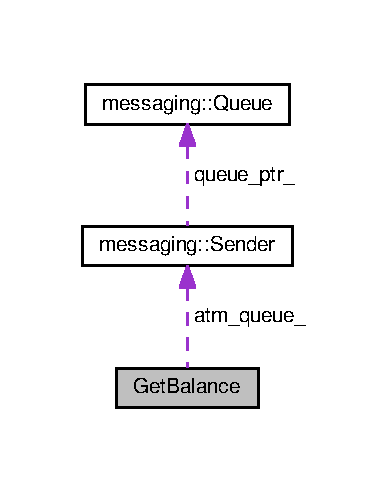
\includegraphics[width=187pt]{structGetBalance__coll__graph}
\end{center}
\end{figure}
\subsection*{Public Member Functions}
\begin{DoxyCompactItemize}
\item 
\hyperlink{structGetBalance_a3c9b1bdf591755a52784b97de5ffd866}{Get\-Balance} (const std\-::string \&account, \hyperlink{classmessaging_1_1Sender}{messaging\-::\-Sender} atm\-\_\-queue)
\end{DoxyCompactItemize}
\subsection*{Public Attributes}
\begin{DoxyCompactItemize}
\item 
std\-::string \hyperlink{structGetBalance_a75b798e4035cf6468cc359db6ba0a4e9}{account\-\_\-}
\item 
\hyperlink{classmessaging_1_1Sender}{messaging\-::\-Sender} \hyperlink{structGetBalance_a469a494592b15655be79bc85c7202750}{atm\-\_\-queue\-\_\-}
\end{DoxyCompactItemize}


\subsection{Constructor \& Destructor Documentation}
\hypertarget{structGetBalance_a3c9b1bdf591755a52784b97de5ffd866}{\index{Get\-Balance@{Get\-Balance}!Get\-Balance@{Get\-Balance}}
\index{Get\-Balance@{Get\-Balance}!GetBalance@{Get\-Balance}}
\subsubsection[{Get\-Balance}]{\setlength{\rightskip}{0pt plus 5cm}Get\-Balance\-::\-Get\-Balance (
\begin{DoxyParamCaption}
\item[{const std\-::string \&}]{account, }
\item[{{\bf messaging\-::\-Sender}}]{atm\-\_\-queue}
\end{DoxyParamCaption}
)\hspace{0.3cm}{\ttfamily [inline]}}}\label{structGetBalance_a3c9b1bdf591755a52784b97de5ffd866}


\subsection{Member Data Documentation}
\hypertarget{structGetBalance_a75b798e4035cf6468cc359db6ba0a4e9}{\index{Get\-Balance@{Get\-Balance}!account\-\_\-@{account\-\_\-}}
\index{account\-\_\-@{account\-\_\-}!GetBalance@{Get\-Balance}}
\subsubsection[{account\-\_\-}]{\setlength{\rightskip}{0pt plus 5cm}std\-::string Get\-Balance\-::account\-\_\-}}\label{structGetBalance_a75b798e4035cf6468cc359db6ba0a4e9}
\hypertarget{structGetBalance_a469a494592b15655be79bc85c7202750}{\index{Get\-Balance@{Get\-Balance}!atm\-\_\-queue\-\_\-@{atm\-\_\-queue\-\_\-}}
\index{atm\-\_\-queue\-\_\-@{atm\-\_\-queue\-\_\-}!GetBalance@{Get\-Balance}}
\subsubsection[{atm\-\_\-queue\-\_\-}]{\setlength{\rightskip}{0pt plus 5cm}{\bf messaging\-::\-Sender} Get\-Balance\-::atm\-\_\-queue\-\_\-\hspace{0.3cm}{\ttfamily [mutable]}}}\label{structGetBalance_a469a494592b15655be79bc85c7202750}


The documentation for this struct was generated from the following file\-:\begin{DoxyCompactItemize}
\item 
/root/\-Public/shack/atm/\hyperlink{withdraw_8h}{withdraw.\-h}\end{DoxyCompactItemize}

\hypertarget{classInterfaceMachine}{\section{Interface\-Machine Class Reference}
\label{classInterfaceMachine}\index{Interface\-Machine@{Interface\-Machine}}
}


{\ttfamily \#include $<$interface\-\_\-machine.\-h$>$}



Collaboration diagram for Interface\-Machine\-:
\nopagebreak
\begin{figure}[H]
\begin{center}
\leavevmode
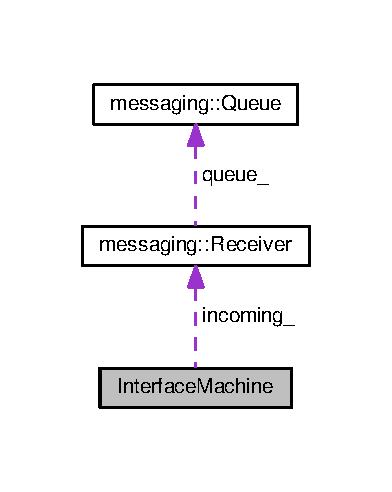
\includegraphics[width=188pt]{classInterfaceMachine__coll__graph}
\end{center}
\end{figure}
\subsection*{Public Member Functions}
\begin{DoxyCompactItemize}
\item 
void \hyperlink{classInterfaceMachine_acfe81f2fdc61f1136d754b8f239e57ea}{Done} ()
\item 
void \hyperlink{classInterfaceMachine_a046f9d3bb23bf7e0b53e68ad152d755d}{Run} ()
\item 
\hyperlink{classmessaging_1_1Sender}{messaging\-::\-Sender} \hyperlink{classInterfaceMachine_a9b431c811e91a9a33254151b1734fd3a}{Get\-Sender} ()
\end{DoxyCompactItemize}
\subsection*{Private Attributes}
\begin{DoxyCompactItemize}
\item 
std\-::mutex \hyperlink{classInterfaceMachine_a00f26d214b26780bca26e8033d2d4921}{io\-\_\-mutex\-\_\-}
\item 
\hyperlink{classmessaging_1_1Receiver}{messaging\-::\-Receiver} \hyperlink{classInterfaceMachine_a9a6baaba223e2a23ead6e80d25c02c59}{incoming\-\_\-}
\end{DoxyCompactItemize}


\subsection{Member Function Documentation}
\hypertarget{classInterfaceMachine_acfe81f2fdc61f1136d754b8f239e57ea}{\index{Interface\-Machine@{Interface\-Machine}!Done@{Done}}
\index{Done@{Done}!InterfaceMachine@{Interface\-Machine}}
\subsubsection[{Done}]{\setlength{\rightskip}{0pt plus 5cm}void Interface\-Machine\-::\-Done (
\begin{DoxyParamCaption}
{}
\end{DoxyParamCaption}
)\hspace{0.3cm}{\ttfamily [inline]}}}\label{classInterfaceMachine_acfe81f2fdc61f1136d754b8f239e57ea}


Here is the call graph for this function\-:\nopagebreak
\begin{figure}[H]
\begin{center}
\leavevmode
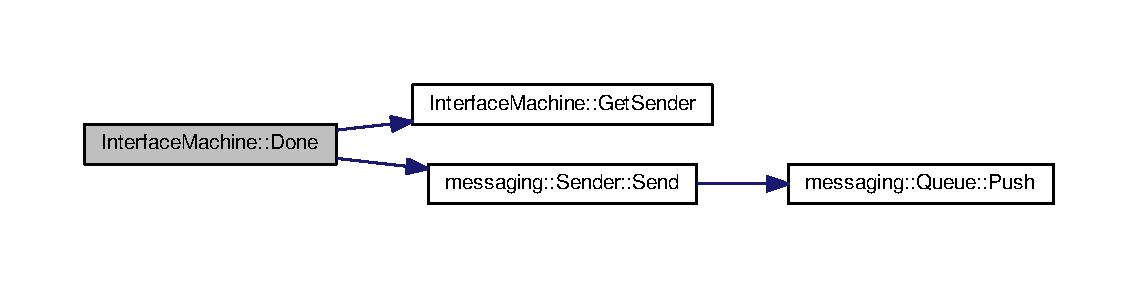
\includegraphics[width=350pt]{classInterfaceMachine_acfe81f2fdc61f1136d754b8f239e57ea_cgraph}
\end{center}
\end{figure}


\hypertarget{classInterfaceMachine_a9b431c811e91a9a33254151b1734fd3a}{\index{Interface\-Machine@{Interface\-Machine}!Get\-Sender@{Get\-Sender}}
\index{Get\-Sender@{Get\-Sender}!InterfaceMachine@{Interface\-Machine}}
\subsubsection[{Get\-Sender}]{\setlength{\rightskip}{0pt plus 5cm}{\bf messaging\-::\-Sender} Interface\-Machine\-::\-Get\-Sender (
\begin{DoxyParamCaption}
{}
\end{DoxyParamCaption}
)\hspace{0.3cm}{\ttfamily [inline]}}}\label{classInterfaceMachine_a9b431c811e91a9a33254151b1734fd3a}
\hypertarget{classInterfaceMachine_a046f9d3bb23bf7e0b53e68ad152d755d}{\index{Interface\-Machine@{Interface\-Machine}!Run@{Run}}
\index{Run@{Run}!InterfaceMachine@{Interface\-Machine}}
\subsubsection[{Run}]{\setlength{\rightskip}{0pt plus 5cm}void Interface\-Machine\-::\-Run (
\begin{DoxyParamCaption}
{}
\end{DoxyParamCaption}
)\hspace{0.3cm}{\ttfamily [inline]}}}\label{classInterfaceMachine_a046f9d3bb23bf7e0b53e68ad152d755d}


Here is the call graph for this function\-:\nopagebreak
\begin{figure}[H]
\begin{center}
\leavevmode
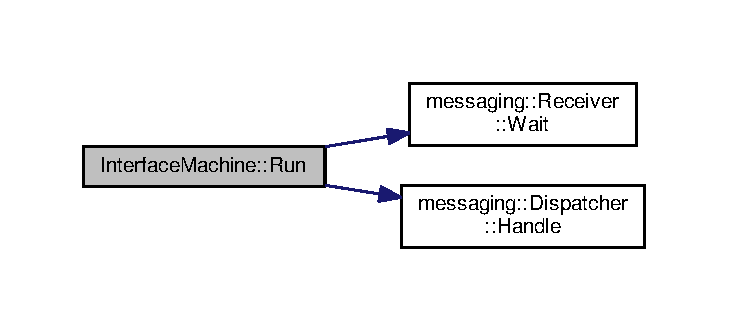
\includegraphics[width=350pt]{classInterfaceMachine_a046f9d3bb23bf7e0b53e68ad152d755d_cgraph}
\end{center}
\end{figure}




\subsection{Member Data Documentation}
\hypertarget{classInterfaceMachine_a9a6baaba223e2a23ead6e80d25c02c59}{\index{Interface\-Machine@{Interface\-Machine}!incoming\-\_\-@{incoming\-\_\-}}
\index{incoming\-\_\-@{incoming\-\_\-}!InterfaceMachine@{Interface\-Machine}}
\subsubsection[{incoming\-\_\-}]{\setlength{\rightskip}{0pt plus 5cm}{\bf messaging\-::\-Receiver} Interface\-Machine\-::incoming\-\_\-\hspace{0.3cm}{\ttfamily [private]}}}\label{classInterfaceMachine_a9a6baaba223e2a23ead6e80d25c02c59}
\hypertarget{classInterfaceMachine_a00f26d214b26780bca26e8033d2d4921}{\index{Interface\-Machine@{Interface\-Machine}!io\-\_\-mutex\-\_\-@{io\-\_\-mutex\-\_\-}}
\index{io\-\_\-mutex\-\_\-@{io\-\_\-mutex\-\_\-}!InterfaceMachine@{Interface\-Machine}}
\subsubsection[{io\-\_\-mutex\-\_\-}]{\setlength{\rightskip}{0pt plus 5cm}std\-::mutex Interface\-Machine\-::io\-\_\-mutex\-\_\-\hspace{0.3cm}{\ttfamily [private]}}}\label{classInterfaceMachine_a00f26d214b26780bca26e8033d2d4921}


The documentation for this class was generated from the following file\-:\begin{DoxyCompactItemize}
\item 
/root/\-Public/shack/atm/\hyperlink{interface__machine_8h}{interface\-\_\-machine.\-h}\end{DoxyCompactItemize}

\hypertarget{structIssueMoney}{\section{Issue\-Money Struct Reference}
\label{structIssueMoney}\index{Issue\-Money@{Issue\-Money}}
}


{\ttfamily \#include $<$withdraw.\-h$>$}

\subsection*{Public Member Functions}
\begin{DoxyCompactItemize}
\item 
\hyperlink{structIssueMoney_a955c7f727bcedad1929ab4e4240f3e0d}{Issue\-Money} (unsigned amount)
\end{DoxyCompactItemize}
\subsection*{Public Attributes}
\begin{DoxyCompactItemize}
\item 
unsigned \hyperlink{structIssueMoney_a79a87d91b556fa635ad61ad654635c76}{amount\-\_\-}
\end{DoxyCompactItemize}


\subsection{Constructor \& Destructor Documentation}
\hypertarget{structIssueMoney_a955c7f727bcedad1929ab4e4240f3e0d}{\index{Issue\-Money@{Issue\-Money}!Issue\-Money@{Issue\-Money}}
\index{Issue\-Money@{Issue\-Money}!IssueMoney@{Issue\-Money}}
\subsubsection[{Issue\-Money}]{\setlength{\rightskip}{0pt plus 5cm}Issue\-Money\-::\-Issue\-Money (
\begin{DoxyParamCaption}
\item[{unsigned}]{amount}
\end{DoxyParamCaption}
)\hspace{0.3cm}{\ttfamily [inline]}}}\label{structIssueMoney_a955c7f727bcedad1929ab4e4240f3e0d}


\subsection{Member Data Documentation}
\hypertarget{structIssueMoney_a79a87d91b556fa635ad61ad654635c76}{\index{Issue\-Money@{Issue\-Money}!amount\-\_\-@{amount\-\_\-}}
\index{amount\-\_\-@{amount\-\_\-}!IssueMoney@{Issue\-Money}}
\subsubsection[{amount\-\_\-}]{\setlength{\rightskip}{0pt plus 5cm}unsigned Issue\-Money\-::amount\-\_\-}}\label{structIssueMoney_a79a87d91b556fa635ad61ad654635c76}


The documentation for this struct was generated from the following file\-:\begin{DoxyCompactItemize}
\item 
/root/\-Public/shack/atm/\hyperlink{withdraw_8h}{withdraw.\-h}\end{DoxyCompactItemize}

\hypertarget{structmessaging_1_1MessageBase}{\section{messaging\-:\-:Message\-Base Struct Reference}
\label{structmessaging_1_1MessageBase}\index{messaging\-::\-Message\-Base@{messaging\-::\-Message\-Base}}
}


{\ttfamily \#include $<$queue.\-h$>$}



Inheritance diagram for messaging\-:\-:Message\-Base\-:\nopagebreak
\begin{figure}[H]
\begin{center}
\leavevmode
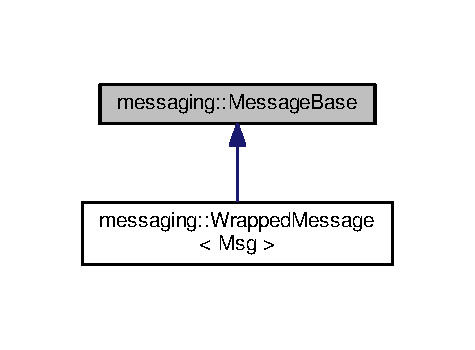
\includegraphics[width=228pt]{structmessaging_1_1MessageBase__inherit__graph}
\end{center}
\end{figure}
\subsection*{Public Member Functions}
\begin{DoxyCompactItemize}
\item 
virtual \hyperlink{structmessaging_1_1MessageBase_afe3211ee077797d75b5a6c549e2aff5f}{$\sim$\-Message\-Base} ()
\end{DoxyCompactItemize}


\subsection{Constructor \& Destructor Documentation}
\hypertarget{structmessaging_1_1MessageBase_afe3211ee077797d75b5a6c549e2aff5f}{\index{messaging\-::\-Message\-Base@{messaging\-::\-Message\-Base}!$\sim$\-Message\-Base@{$\sim$\-Message\-Base}}
\index{$\sim$\-Message\-Base@{$\sim$\-Message\-Base}!messaging::MessageBase@{messaging\-::\-Message\-Base}}
\subsubsection[{$\sim$\-Message\-Base}]{\setlength{\rightskip}{0pt plus 5cm}virtual messaging\-::\-Message\-Base\-::$\sim$\-Message\-Base (
\begin{DoxyParamCaption}
{}
\end{DoxyParamCaption}
)\hspace{0.3cm}{\ttfamily [inline]}, {\ttfamily [virtual]}}}\label{structmessaging_1_1MessageBase_afe3211ee077797d75b5a6c549e2aff5f}


The documentation for this struct was generated from the following file\-:\begin{DoxyCompactItemize}
\item 
/root/\-Public/shack/atm/\hyperlink{queue_8h}{queue.\-h}\end{DoxyCompactItemize}

\hypertarget{structPinIncorrect}{\section{Pin\-Incorrect Struct Reference}
\label{structPinIncorrect}\index{Pin\-Incorrect@{Pin\-Incorrect}}
}


{\ttfamily \#include $<$withdraw.\-h$>$}



The documentation for this struct was generated from the following file\-:\begin{DoxyCompactItemize}
\item 
/root/\-Public/shack/atm/\hyperlink{withdraw_8h}{withdraw.\-h}\end{DoxyCompactItemize}

\hypertarget{structPinVerified}{\section{Pin\-Verified Struct Reference}
\label{structPinVerified}\index{Pin\-Verified@{Pin\-Verified}}
}


{\ttfamily \#include $<$withdraw.\-h$>$}



The documentation for this struct was generated from the following file\-:\begin{DoxyCompactItemize}
\item 
/root/\-Public/shack/atm/\hyperlink{withdraw_8h}{withdraw.\-h}\end{DoxyCompactItemize}

\hypertarget{classmessaging_1_1Queue}{\section{messaging\-:\-:Queue Class Reference}
\label{classmessaging_1_1Queue}\index{messaging\-::\-Queue@{messaging\-::\-Queue}}
}


{\ttfamily \#include $<$queue.\-h$>$}

\subsection*{Public Member Functions}
\begin{DoxyCompactItemize}
\item 
{\footnotesize template$<$class T $>$ }\\void \hyperlink{classmessaging_1_1Queue_a8ee0ac353ead8aca910d8073a2d5e16e}{Push} (const T \&msg)
\item 
std\-::shared\-\_\-ptr$<$ \hyperlink{structmessaging_1_1MessageBase}{Message\-Base} $>$ \hyperlink{classmessaging_1_1Queue_a624adbac8b7f4b5ebf6bb0f9ab76bcc3}{Wait\-And\-Pop} ()
\end{DoxyCompactItemize}
\subsection*{Private Attributes}
\begin{DoxyCompactItemize}
\item 
std\-::mutex \hyperlink{classmessaging_1_1Queue_acb84af14fea49c09597be7ad19f9f3c5}{mutex\-\_\-}
\item 
std\-::condition\-\_\-variable \hyperlink{classmessaging_1_1Queue_aec7510ebff3d15176afdf3d93ca6fdc8}{cond\-\_\-var\-\_\-}
\item 
std\-::queue$<$ std\-::shared\-\_\-ptr\\*
$<$ \hyperlink{structmessaging_1_1MessageBase}{Message\-Base} $>$ $>$ \hyperlink{classmessaging_1_1Queue_aae9c5f0bc7b5be870129c56643404551}{queue\-\_\-}
\end{DoxyCompactItemize}


\subsection{Member Function Documentation}
\hypertarget{classmessaging_1_1Queue_a8ee0ac353ead8aca910d8073a2d5e16e}{\index{messaging\-::\-Queue@{messaging\-::\-Queue}!Push@{Push}}
\index{Push@{Push}!messaging::Queue@{messaging\-::\-Queue}}
\subsubsection[{Push}]{\setlength{\rightskip}{0pt plus 5cm}template$<$class T $>$ void messaging\-::\-Queue\-::\-Push (
\begin{DoxyParamCaption}
\item[{const T \&}]{msg}
\end{DoxyParamCaption}
)\hspace{0.3cm}{\ttfamily [inline]}}}\label{classmessaging_1_1Queue_a8ee0ac353ead8aca910d8073a2d5e16e}
\hypertarget{classmessaging_1_1Queue_a624adbac8b7f4b5ebf6bb0f9ab76bcc3}{\index{messaging\-::\-Queue@{messaging\-::\-Queue}!Wait\-And\-Pop@{Wait\-And\-Pop}}
\index{Wait\-And\-Pop@{Wait\-And\-Pop}!messaging::Queue@{messaging\-::\-Queue}}
\subsubsection[{Wait\-And\-Pop}]{\setlength{\rightskip}{0pt plus 5cm}std\-::shared\-\_\-ptr$<${\bf Message\-Base}$>$ messaging\-::\-Queue\-::\-Wait\-And\-Pop (
\begin{DoxyParamCaption}
{}
\end{DoxyParamCaption}
)\hspace{0.3cm}{\ttfamily [inline]}}}\label{classmessaging_1_1Queue_a624adbac8b7f4b5ebf6bb0f9ab76bcc3}


\subsection{Member Data Documentation}
\hypertarget{classmessaging_1_1Queue_aec7510ebff3d15176afdf3d93ca6fdc8}{\index{messaging\-::\-Queue@{messaging\-::\-Queue}!cond\-\_\-var\-\_\-@{cond\-\_\-var\-\_\-}}
\index{cond\-\_\-var\-\_\-@{cond\-\_\-var\-\_\-}!messaging::Queue@{messaging\-::\-Queue}}
\subsubsection[{cond\-\_\-var\-\_\-}]{\setlength{\rightskip}{0pt plus 5cm}std\-::condition\-\_\-variable messaging\-::\-Queue\-::cond\-\_\-var\-\_\-\hspace{0.3cm}{\ttfamily [private]}}}\label{classmessaging_1_1Queue_aec7510ebff3d15176afdf3d93ca6fdc8}
\hypertarget{classmessaging_1_1Queue_acb84af14fea49c09597be7ad19f9f3c5}{\index{messaging\-::\-Queue@{messaging\-::\-Queue}!mutex\-\_\-@{mutex\-\_\-}}
\index{mutex\-\_\-@{mutex\-\_\-}!messaging::Queue@{messaging\-::\-Queue}}
\subsubsection[{mutex\-\_\-}]{\setlength{\rightskip}{0pt plus 5cm}std\-::mutex messaging\-::\-Queue\-::mutex\-\_\-\hspace{0.3cm}{\ttfamily [private]}}}\label{classmessaging_1_1Queue_acb84af14fea49c09597be7ad19f9f3c5}
\hypertarget{classmessaging_1_1Queue_aae9c5f0bc7b5be870129c56643404551}{\index{messaging\-::\-Queue@{messaging\-::\-Queue}!queue\-\_\-@{queue\-\_\-}}
\index{queue\-\_\-@{queue\-\_\-}!messaging::Queue@{messaging\-::\-Queue}}
\subsubsection[{queue\-\_\-}]{\setlength{\rightskip}{0pt plus 5cm}std\-::queue$<$std\-::shared\-\_\-ptr$<${\bf Message\-Base}$>$ $>$ messaging\-::\-Queue\-::queue\-\_\-\hspace{0.3cm}{\ttfamily [private]}}}\label{classmessaging_1_1Queue_aae9c5f0bc7b5be870129c56643404551}


The documentation for this class was generated from the following file\-:\begin{DoxyCompactItemize}
\item 
/root/\-Public/shack/atm/\hyperlink{queue_8h}{queue.\-h}\end{DoxyCompactItemize}

\hypertarget{classmessaging_1_1Receiver}{\section{messaging\-:\-:Receiver Class Reference}
\label{classmessaging_1_1Receiver}\index{messaging\-::\-Receiver@{messaging\-::\-Receiver}}
}


{\ttfamily \#include $<$receiver.\-h$>$}



Collaboration diagram for messaging\-:\-:Receiver\-:
\nopagebreak
\begin{figure}[H]
\begin{center}
\leavevmode
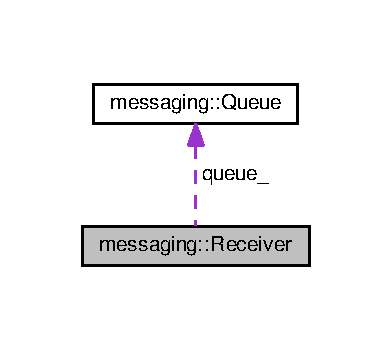
\includegraphics[width=188pt]{classmessaging_1_1Receiver__coll__graph}
\end{center}
\end{figure}
\subsection*{Public Member Functions}
\begin{DoxyCompactItemize}
\item 
\hyperlink{classmessaging_1_1Receiver_a032cf4096825d90ae51404c8655db6f0}{operator Sender} ()
\item 
\hyperlink{classmessaging_1_1Dispatcher}{Dispatcher} \hyperlink{classmessaging_1_1Receiver_a3f0e7b541159793eaec1e0fa6802d4d2}{Wait} ()
\end{DoxyCompactItemize}
\subsection*{Private Attributes}
\begin{DoxyCompactItemize}
\item 
\hyperlink{classmessaging_1_1Queue}{Queue} \hyperlink{classmessaging_1_1Receiver_a5d1deaa42acaabf2837860e9672dc2d3}{queue\-\_\-}
\end{DoxyCompactItemize}


\subsection{Member Function Documentation}
\hypertarget{classmessaging_1_1Receiver_a032cf4096825d90ae51404c8655db6f0}{\index{messaging\-::\-Receiver@{messaging\-::\-Receiver}!operator Sender@{operator Sender}}
\index{operator Sender@{operator Sender}!messaging::Receiver@{messaging\-::\-Receiver}}
\subsubsection[{operator Sender}]{\setlength{\rightskip}{0pt plus 5cm}messaging\-::\-Receiver\-::operator {\bf Sender} (
\begin{DoxyParamCaption}
{}
\end{DoxyParamCaption}
)\hspace{0.3cm}{\ttfamily [inline]}}}\label{classmessaging_1_1Receiver_a032cf4096825d90ae51404c8655db6f0}
\hypertarget{classmessaging_1_1Receiver_a3f0e7b541159793eaec1e0fa6802d4d2}{\index{messaging\-::\-Receiver@{messaging\-::\-Receiver}!Wait@{Wait}}
\index{Wait@{Wait}!messaging::Receiver@{messaging\-::\-Receiver}}
\subsubsection[{Wait}]{\setlength{\rightskip}{0pt plus 5cm}{\bf Dispatcher} messaging\-::\-Receiver\-::\-Wait (
\begin{DoxyParamCaption}
{}
\end{DoxyParamCaption}
)\hspace{0.3cm}{\ttfamily [inline]}}}\label{classmessaging_1_1Receiver_a3f0e7b541159793eaec1e0fa6802d4d2}


\subsection{Member Data Documentation}
\hypertarget{classmessaging_1_1Receiver_a5d1deaa42acaabf2837860e9672dc2d3}{\index{messaging\-::\-Receiver@{messaging\-::\-Receiver}!queue\-\_\-@{queue\-\_\-}}
\index{queue\-\_\-@{queue\-\_\-}!messaging::Receiver@{messaging\-::\-Receiver}}
\subsubsection[{queue\-\_\-}]{\setlength{\rightskip}{0pt plus 5cm}{\bf Queue} messaging\-::\-Receiver\-::queue\-\_\-\hspace{0.3cm}{\ttfamily [private]}}}\label{classmessaging_1_1Receiver_a5d1deaa42acaabf2837860e9672dc2d3}


The documentation for this class was generated from the following file\-:\begin{DoxyCompactItemize}
\item 
/root/\-Public/shack/atm/\hyperlink{receiver_8h}{receiver.\-h}\end{DoxyCompactItemize}

\hypertarget{classmessaging_1_1Sender}{\section{messaging\-:\-:Sender Class Reference}
\label{classmessaging_1_1Sender}\index{messaging\-::\-Sender@{messaging\-::\-Sender}}
}


{\ttfamily \#include $<$sender.\-h$>$}



Collaboration diagram for messaging\-:\-:Sender\-:
\nopagebreak
\begin{figure}[H]
\begin{center}
\leavevmode
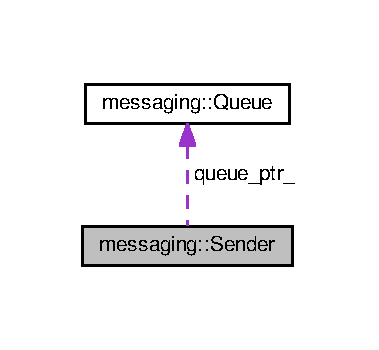
\includegraphics[width=182pt]{classmessaging_1_1Sender__coll__graph}
\end{center}
\end{figure}
\subsection*{Public Member Functions}
\begin{DoxyCompactItemize}
\item 
\hyperlink{classmessaging_1_1Sender_a40d7ba2c5bd94d249b47b518466870dc}{Sender} ()
\item 
\hyperlink{classmessaging_1_1Sender_a55b2718ff332f741494d3d90c7b83de2}{Sender} (\hyperlink{classmessaging_1_1Queue}{Queue} $\ast$queue\-\_\-ptr)
\item 
{\footnotesize template$<$class Message $>$ }\\void \hyperlink{classmessaging_1_1Sender_a5f8d8f2fa560996d8f224cc0f10d8f8c}{Send} (const Message \&msg)
\end{DoxyCompactItemize}
\subsection*{Private Attributes}
\begin{DoxyCompactItemize}
\item 
\hyperlink{classmessaging_1_1Queue}{Queue} $\ast$ \hyperlink{classmessaging_1_1Sender_a56aa7e425615eae331039cd66346b56c}{queue\-\_\-ptr\-\_\-}
\end{DoxyCompactItemize}


\subsection{Constructor \& Destructor Documentation}
\hypertarget{classmessaging_1_1Sender_a40d7ba2c5bd94d249b47b518466870dc}{\index{messaging\-::\-Sender@{messaging\-::\-Sender}!Sender@{Sender}}
\index{Sender@{Sender}!messaging::Sender@{messaging\-::\-Sender}}
\subsubsection[{Sender}]{\setlength{\rightskip}{0pt plus 5cm}messaging\-::\-Sender\-::\-Sender (
\begin{DoxyParamCaption}
{}
\end{DoxyParamCaption}
)\hspace{0.3cm}{\ttfamily [inline]}}}\label{classmessaging_1_1Sender_a40d7ba2c5bd94d249b47b518466870dc}
\hypertarget{classmessaging_1_1Sender_a55b2718ff332f741494d3d90c7b83de2}{\index{messaging\-::\-Sender@{messaging\-::\-Sender}!Sender@{Sender}}
\index{Sender@{Sender}!messaging::Sender@{messaging\-::\-Sender}}
\subsubsection[{Sender}]{\setlength{\rightskip}{0pt plus 5cm}messaging\-::\-Sender\-::\-Sender (
\begin{DoxyParamCaption}
\item[{{\bf Queue} $\ast$}]{queue\-\_\-ptr}
\end{DoxyParamCaption}
)\hspace{0.3cm}{\ttfamily [inline]}, {\ttfamily [explicit]}}}\label{classmessaging_1_1Sender_a55b2718ff332f741494d3d90c7b83de2}


\subsection{Member Function Documentation}
\hypertarget{classmessaging_1_1Sender_a5f8d8f2fa560996d8f224cc0f10d8f8c}{\index{messaging\-::\-Sender@{messaging\-::\-Sender}!Send@{Send}}
\index{Send@{Send}!messaging::Sender@{messaging\-::\-Sender}}
\subsubsection[{Send}]{\setlength{\rightskip}{0pt plus 5cm}template$<$class Message $>$ void messaging\-::\-Sender\-::\-Send (
\begin{DoxyParamCaption}
\item[{const Message \&}]{msg}
\end{DoxyParamCaption}
)\hspace{0.3cm}{\ttfamily [inline]}}}\label{classmessaging_1_1Sender_a5f8d8f2fa560996d8f224cc0f10d8f8c}


Here is the call graph for this function\-:\nopagebreak
\begin{figure}[H]
\begin{center}
\leavevmode
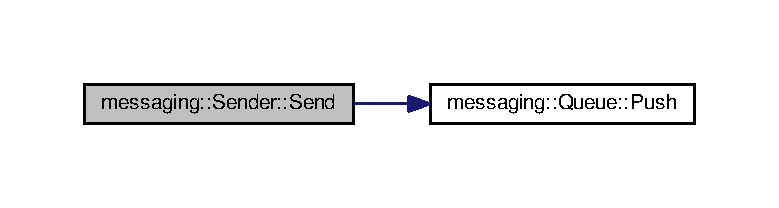
\includegraphics[width=350pt]{classmessaging_1_1Sender_a5f8d8f2fa560996d8f224cc0f10d8f8c_cgraph}
\end{center}
\end{figure}




\subsection{Member Data Documentation}
\hypertarget{classmessaging_1_1Sender_a56aa7e425615eae331039cd66346b56c}{\index{messaging\-::\-Sender@{messaging\-::\-Sender}!queue\-\_\-ptr\-\_\-@{queue\-\_\-ptr\-\_\-}}
\index{queue\-\_\-ptr\-\_\-@{queue\-\_\-ptr\-\_\-}!messaging::Sender@{messaging\-::\-Sender}}
\subsubsection[{queue\-\_\-ptr\-\_\-}]{\setlength{\rightskip}{0pt plus 5cm}{\bf Queue}$\ast$ messaging\-::\-Sender\-::queue\-\_\-ptr\-\_\-\hspace{0.3cm}{\ttfamily [private]}}}\label{classmessaging_1_1Sender_a56aa7e425615eae331039cd66346b56c}


The documentation for this class was generated from the following file\-:\begin{DoxyCompactItemize}
\item 
/root/\-Public/shack/atm/\hyperlink{sender_8h}{sender.\-h}\end{DoxyCompactItemize}

\hypertarget{classmessaging_1_1TemplateDispatcher}{\section{messaging\-:\-:Template\-Dispatcher$<$ Previous\-Dispatcher, Msg, Func $>$ Class Template Reference}
\label{classmessaging_1_1TemplateDispatcher}\index{messaging\-::\-Template\-Dispatcher$<$ Previous\-Dispatcher, Msg, Func $>$@{messaging\-::\-Template\-Dispatcher$<$ Previous\-Dispatcher, Msg, Func $>$}}
}


{\ttfamily \#include $<$template\-\_\-dispatcher.\-h$>$}



Collaboration diagram for messaging\-:\-:Template\-Dispatcher$<$ Previous\-Dispatcher, Msg, Func $>$\-:
\nopagebreak
\begin{figure}[H]
\begin{center}
\leavevmode
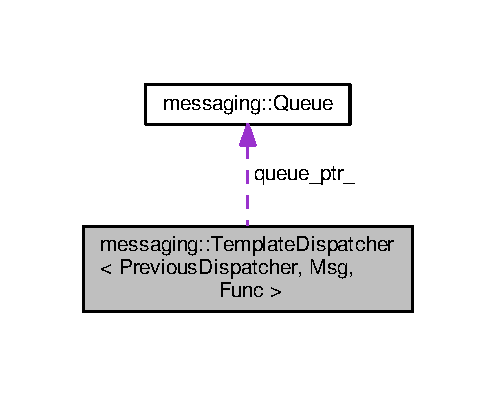
\includegraphics[width=238pt]{classmessaging_1_1TemplateDispatcher__coll__graph}
\end{center}
\end{figure}
\subsection*{Public Member Functions}
\begin{DoxyCompactItemize}
\item 
\hyperlink{classmessaging_1_1TemplateDispatcher_ada53b5ba67f04fa2a8420cded172fdd1}{Template\-Dispatcher} (\hyperlink{classmessaging_1_1TemplateDispatcher}{Template\-Dispatcher} \&\&other)
\item 
\hyperlink{classmessaging_1_1TemplateDispatcher_a00aff7fdf1654ddfc2389d719b949427}{Template\-Dispatcher} (\hyperlink{classmessaging_1_1Queue}{Queue} $\ast$queue, Previous\-Dispatcher $\ast$prev\-\_\-ptr, Func \&\&func)
\item 
\hyperlink{classmessaging_1_1TemplateDispatcher_a7ef05880e531ba95632f7c7e0c78f4a3}{Template\-Dispatcher} (const \hyperlink{classmessaging_1_1TemplateDispatcher}{Template\-Dispatcher} \&)=delete
\item 
\hyperlink{classmessaging_1_1TemplateDispatcher}{Template\-Dispatcher} \& \hyperlink{classmessaging_1_1TemplateDispatcher_a5d5e246da02eb04699e03cf40a129076}{operator=} (const \hyperlink{classmessaging_1_1TemplateDispatcher}{Template\-Dispatcher} \&)=delete
\item 
{\footnotesize template$<$class Other\-Msg , class Other\-Func $>$ }\\\hyperlink{classmessaging_1_1TemplateDispatcher}{Template\-Dispatcher}\\*
$<$ \hyperlink{classmessaging_1_1TemplateDispatcher}{Template\-Dispatcher}, Other\-Msg, \\*
Other\-Func $>$ \hyperlink{classmessaging_1_1TemplateDispatcher_a06911b99af5573acede1d78ab6c4aa4f}{Handle} (Other\-Func \&\&other\-\_\-func)
\item 
\hyperlink{classmessaging_1_1TemplateDispatcher_abf090c18964d34afd84af5e03e90d9b7}{$\sim$\-Template\-Dispatcher} () noexcept(false)
\end{DoxyCompactItemize}
\subsection*{Private Member Functions}
\begin{DoxyCompactItemize}
\item 
void \hyperlink{classmessaging_1_1TemplateDispatcher_ab36064e19b91ff2ea8f37034b8de7f60}{Wait\-And\-Dispatch} ()
\item 
bool \hyperlink{classmessaging_1_1TemplateDispatcher_a0e8673cb9d39a44f0a8332885efbde8d}{Dispatch} (const std\-::shared\-\_\-ptr$<$ \hyperlink{structmessaging_1_1MessageBase}{Message\-Base} $>$ \&msg)
\end{DoxyCompactItemize}
\subsection*{Private Attributes}
\begin{DoxyCompactItemize}
\item 
\hyperlink{classmessaging_1_1Queue}{Queue} $\ast$ \hyperlink{classmessaging_1_1TemplateDispatcher_a1c84a8173b54823d7b95db4d4865e134}{queue\-\_\-ptr\-\_\-}
\item 
Previous\-Dispatcher $\ast$ \hyperlink{classmessaging_1_1TemplateDispatcher_a873bc46a8c8cff1ddcceb225ad252e01}{prev\-\_\-ptr\-\_\-}
\item 
Func \hyperlink{classmessaging_1_1TemplateDispatcher_aae5b9ea3d2b58005b6ddec368db2bcb0}{func\-\_\-}
\item 
bool \hyperlink{classmessaging_1_1TemplateDispatcher_a51f4255d452392ab1ca7d193d3209d4a}{chained\-\_\-}
\end{DoxyCompactItemize}
\subsection*{Friends}
\begin{DoxyCompactItemize}
\item 
{\footnotesize template$<$class Dispatcher , class Other\-Msg , class Other\-Func $>$ }\\class \hyperlink{classmessaging_1_1TemplateDispatcher_ac52eebabf93ac84bc8eacc5c67e6ca9f}{Template\-Dispatcher}
\end{DoxyCompactItemize}


\subsection{Constructor \& Destructor Documentation}
\hypertarget{classmessaging_1_1TemplateDispatcher_ada53b5ba67f04fa2a8420cded172fdd1}{\index{messaging\-::\-Template\-Dispatcher@{messaging\-::\-Template\-Dispatcher}!Template\-Dispatcher@{Template\-Dispatcher}}
\index{Template\-Dispatcher@{Template\-Dispatcher}!messaging::TemplateDispatcher@{messaging\-::\-Template\-Dispatcher}}
\subsubsection[{Template\-Dispatcher}]{\setlength{\rightskip}{0pt plus 5cm}template$<$class Previous\-Dispatcher, class Msg, class Func$>$ {\bf messaging\-::\-Template\-Dispatcher}$<$ Previous\-Dispatcher, Msg, Func $>$\-::{\bf Template\-Dispatcher} (
\begin{DoxyParamCaption}
\item[{{\bf Template\-Dispatcher}$<$ Previous\-Dispatcher, Msg, Func $>$ \&\&}]{other}
\end{DoxyParamCaption}
)\hspace{0.3cm}{\ttfamily [inline]}}}\label{classmessaging_1_1TemplateDispatcher_ada53b5ba67f04fa2a8420cded172fdd1}
\hypertarget{classmessaging_1_1TemplateDispatcher_a00aff7fdf1654ddfc2389d719b949427}{\index{messaging\-::\-Template\-Dispatcher@{messaging\-::\-Template\-Dispatcher}!Template\-Dispatcher@{Template\-Dispatcher}}
\index{Template\-Dispatcher@{Template\-Dispatcher}!messaging::TemplateDispatcher@{messaging\-::\-Template\-Dispatcher}}
\subsubsection[{Template\-Dispatcher}]{\setlength{\rightskip}{0pt plus 5cm}template$<$class Previous\-Dispatcher, class Msg, class Func$>$ {\bf messaging\-::\-Template\-Dispatcher}$<$ Previous\-Dispatcher, Msg, Func $>$\-::{\bf Template\-Dispatcher} (
\begin{DoxyParamCaption}
\item[{{\bf Queue} $\ast$}]{queue, }
\item[{Previous\-Dispatcher $\ast$}]{prev\-\_\-ptr, }
\item[{Func \&\&}]{func}
\end{DoxyParamCaption}
)\hspace{0.3cm}{\ttfamily [inline]}}}\label{classmessaging_1_1TemplateDispatcher_a00aff7fdf1654ddfc2389d719b949427}
\hypertarget{classmessaging_1_1TemplateDispatcher_a7ef05880e531ba95632f7c7e0c78f4a3}{\index{messaging\-::\-Template\-Dispatcher@{messaging\-::\-Template\-Dispatcher}!Template\-Dispatcher@{Template\-Dispatcher}}
\index{Template\-Dispatcher@{Template\-Dispatcher}!messaging::TemplateDispatcher@{messaging\-::\-Template\-Dispatcher}}
\subsubsection[{Template\-Dispatcher}]{\setlength{\rightskip}{0pt plus 5cm}template$<$class Previous\-Dispatcher, class Msg, class Func$>$ {\bf messaging\-::\-Template\-Dispatcher}$<$ Previous\-Dispatcher, Msg, Func $>$\-::{\bf Template\-Dispatcher} (
\begin{DoxyParamCaption}
\item[{const {\bf Template\-Dispatcher}$<$ Previous\-Dispatcher, Msg, Func $>$ \&}]{}
\end{DoxyParamCaption}
)\hspace{0.3cm}{\ttfamily [delete]}}}\label{classmessaging_1_1TemplateDispatcher_a7ef05880e531ba95632f7c7e0c78f4a3}
\hypertarget{classmessaging_1_1TemplateDispatcher_abf090c18964d34afd84af5e03e90d9b7}{\index{messaging\-::\-Template\-Dispatcher@{messaging\-::\-Template\-Dispatcher}!$\sim$\-Template\-Dispatcher@{$\sim$\-Template\-Dispatcher}}
\index{$\sim$\-Template\-Dispatcher@{$\sim$\-Template\-Dispatcher}!messaging::TemplateDispatcher@{messaging\-::\-Template\-Dispatcher}}
\subsubsection[{$\sim$\-Template\-Dispatcher}]{\setlength{\rightskip}{0pt plus 5cm}template$<$class Previous\-Dispatcher, class Msg, class Func$>$ {\bf messaging\-::\-Template\-Dispatcher}$<$ Previous\-Dispatcher, Msg, Func $>$\-::$\sim${\bf Template\-Dispatcher} (
\begin{DoxyParamCaption}
{}
\end{DoxyParamCaption}
)\hspace{0.3cm}{\ttfamily [inline]}, {\ttfamily [noexcept]}}}\label{classmessaging_1_1TemplateDispatcher_abf090c18964d34afd84af5e03e90d9b7}


Here is the call graph for this function\-:
\nopagebreak
\begin{figure}[H]
\begin{center}
\leavevmode
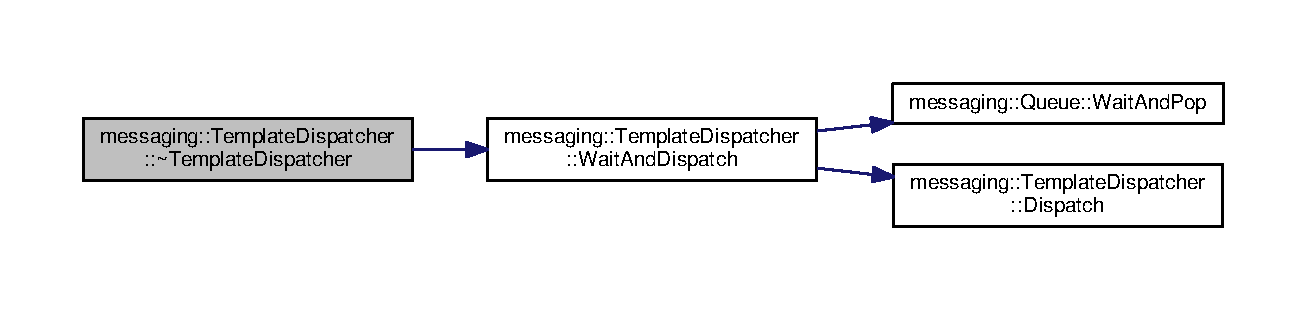
\includegraphics[width=350pt]{classmessaging_1_1TemplateDispatcher_abf090c18964d34afd84af5e03e90d9b7_cgraph}
\end{center}
\end{figure}




\subsection{Member Function Documentation}
\hypertarget{classmessaging_1_1TemplateDispatcher_a0e8673cb9d39a44f0a8332885efbde8d}{\index{messaging\-::\-Template\-Dispatcher@{messaging\-::\-Template\-Dispatcher}!Dispatch@{Dispatch}}
\index{Dispatch@{Dispatch}!messaging::TemplateDispatcher@{messaging\-::\-Template\-Dispatcher}}
\subsubsection[{Dispatch}]{\setlength{\rightskip}{0pt plus 5cm}template$<$class Previous\-Dispatcher, class Msg, class Func$>$ bool {\bf messaging\-::\-Template\-Dispatcher}$<$ Previous\-Dispatcher, Msg, Func $>$\-::Dispatch (
\begin{DoxyParamCaption}
\item[{const std\-::shared\-\_\-ptr$<$ {\bf Message\-Base} $>$ \&}]{msg}
\end{DoxyParamCaption}
)\hspace{0.3cm}{\ttfamily [inline]}, {\ttfamily [private]}}}\label{classmessaging_1_1TemplateDispatcher_a0e8673cb9d39a44f0a8332885efbde8d}
\hypertarget{classmessaging_1_1TemplateDispatcher_a06911b99af5573acede1d78ab6c4aa4f}{\index{messaging\-::\-Template\-Dispatcher@{messaging\-::\-Template\-Dispatcher}!Handle@{Handle}}
\index{Handle@{Handle}!messaging::TemplateDispatcher@{messaging\-::\-Template\-Dispatcher}}
\subsubsection[{Handle}]{\setlength{\rightskip}{0pt plus 5cm}template$<$class Previous\-Dispatcher, class Msg, class Func$>$ template$<$class Other\-Msg , class Other\-Func $>$ {\bf Template\-Dispatcher}$<${\bf Template\-Dispatcher}, Other\-Msg, Other\-Func$>$ {\bf messaging\-::\-Template\-Dispatcher}$<$ Previous\-Dispatcher, Msg, Func $>$\-::Handle (
\begin{DoxyParamCaption}
\item[{Other\-Func \&\&}]{other\-\_\-func}
\end{DoxyParamCaption}
)\hspace{0.3cm}{\ttfamily [inline]}}}\label{classmessaging_1_1TemplateDispatcher_a06911b99af5573acede1d78ab6c4aa4f}
\hypertarget{classmessaging_1_1TemplateDispatcher_a5d5e246da02eb04699e03cf40a129076}{\index{messaging\-::\-Template\-Dispatcher@{messaging\-::\-Template\-Dispatcher}!operator=@{operator=}}
\index{operator=@{operator=}!messaging::TemplateDispatcher@{messaging\-::\-Template\-Dispatcher}}
\subsubsection[{operator=}]{\setlength{\rightskip}{0pt plus 5cm}template$<$class Previous\-Dispatcher, class Msg, class Func$>$ {\bf Template\-Dispatcher}\& {\bf messaging\-::\-Template\-Dispatcher}$<$ Previous\-Dispatcher, Msg, Func $>$\-::operator= (
\begin{DoxyParamCaption}
\item[{const {\bf Template\-Dispatcher}$<$ Previous\-Dispatcher, Msg, Func $>$ \&}]{}
\end{DoxyParamCaption}
)\hspace{0.3cm}{\ttfamily [delete]}}}\label{classmessaging_1_1TemplateDispatcher_a5d5e246da02eb04699e03cf40a129076}
\hypertarget{classmessaging_1_1TemplateDispatcher_ab36064e19b91ff2ea8f37034b8de7f60}{\index{messaging\-::\-Template\-Dispatcher@{messaging\-::\-Template\-Dispatcher}!Wait\-And\-Dispatch@{Wait\-And\-Dispatch}}
\index{Wait\-And\-Dispatch@{Wait\-And\-Dispatch}!messaging::TemplateDispatcher@{messaging\-::\-Template\-Dispatcher}}
\subsubsection[{Wait\-And\-Dispatch}]{\setlength{\rightskip}{0pt plus 5cm}template$<$class Previous\-Dispatcher, class Msg, class Func$>$ void {\bf messaging\-::\-Template\-Dispatcher}$<$ Previous\-Dispatcher, Msg, Func $>$\-::Wait\-And\-Dispatch (
\begin{DoxyParamCaption}
{}
\end{DoxyParamCaption}
)\hspace{0.3cm}{\ttfamily [inline]}, {\ttfamily [private]}}}\label{classmessaging_1_1TemplateDispatcher_ab36064e19b91ff2ea8f37034b8de7f60}


Here is the call graph for this function\-:
\nopagebreak
\begin{figure}[H]
\begin{center}
\leavevmode
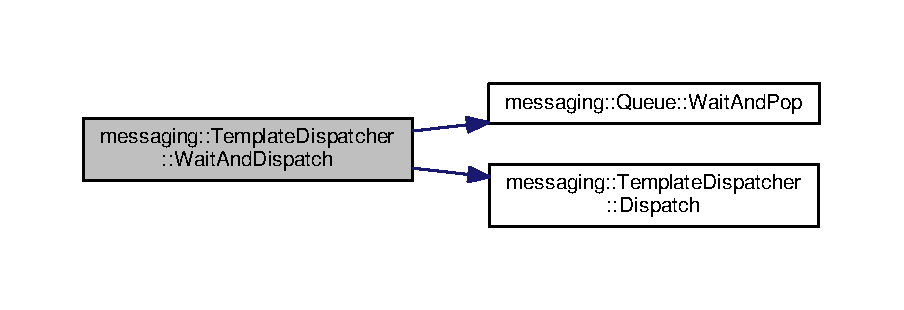
\includegraphics[width=350pt]{classmessaging_1_1TemplateDispatcher_ab36064e19b91ff2ea8f37034b8de7f60_cgraph}
\end{center}
\end{figure}




\subsection{Friends And Related Function Documentation}
\hypertarget{classmessaging_1_1TemplateDispatcher_ac52eebabf93ac84bc8eacc5c67e6ca9f}{\index{messaging\-::\-Template\-Dispatcher@{messaging\-::\-Template\-Dispatcher}!Template\-Dispatcher@{Template\-Dispatcher}}
\index{Template\-Dispatcher@{Template\-Dispatcher}!messaging::TemplateDispatcher@{messaging\-::\-Template\-Dispatcher}}
\subsubsection[{Template\-Dispatcher}]{\setlength{\rightskip}{0pt plus 5cm}template$<$class Previous\-Dispatcher, class Msg, class Func$>$ template$<$class Dispatcher , class Other\-Msg , class Other\-Func $>$ friend class {\bf Template\-Dispatcher}\hspace{0.3cm}{\ttfamily [friend]}}}\label{classmessaging_1_1TemplateDispatcher_ac52eebabf93ac84bc8eacc5c67e6ca9f}


\subsection{Member Data Documentation}
\hypertarget{classmessaging_1_1TemplateDispatcher_a51f4255d452392ab1ca7d193d3209d4a}{\index{messaging\-::\-Template\-Dispatcher@{messaging\-::\-Template\-Dispatcher}!chained\-\_\-@{chained\-\_\-}}
\index{chained\-\_\-@{chained\-\_\-}!messaging::TemplateDispatcher@{messaging\-::\-Template\-Dispatcher}}
\subsubsection[{chained\-\_\-}]{\setlength{\rightskip}{0pt plus 5cm}template$<$class Previous\-Dispatcher, class Msg, class Func$>$ bool {\bf messaging\-::\-Template\-Dispatcher}$<$ Previous\-Dispatcher, Msg, Func $>$\-::chained\-\_\-\hspace{0.3cm}{\ttfamily [private]}}}\label{classmessaging_1_1TemplateDispatcher_a51f4255d452392ab1ca7d193d3209d4a}
\hypertarget{classmessaging_1_1TemplateDispatcher_aae5b9ea3d2b58005b6ddec368db2bcb0}{\index{messaging\-::\-Template\-Dispatcher@{messaging\-::\-Template\-Dispatcher}!func\-\_\-@{func\-\_\-}}
\index{func\-\_\-@{func\-\_\-}!messaging::TemplateDispatcher@{messaging\-::\-Template\-Dispatcher}}
\subsubsection[{func\-\_\-}]{\setlength{\rightskip}{0pt plus 5cm}template$<$class Previous\-Dispatcher, class Msg, class Func$>$ Func {\bf messaging\-::\-Template\-Dispatcher}$<$ Previous\-Dispatcher, Msg, Func $>$\-::func\-\_\-\hspace{0.3cm}{\ttfamily [private]}}}\label{classmessaging_1_1TemplateDispatcher_aae5b9ea3d2b58005b6ddec368db2bcb0}
\hypertarget{classmessaging_1_1TemplateDispatcher_a873bc46a8c8cff1ddcceb225ad252e01}{\index{messaging\-::\-Template\-Dispatcher@{messaging\-::\-Template\-Dispatcher}!prev\-\_\-ptr\-\_\-@{prev\-\_\-ptr\-\_\-}}
\index{prev\-\_\-ptr\-\_\-@{prev\-\_\-ptr\-\_\-}!messaging::TemplateDispatcher@{messaging\-::\-Template\-Dispatcher}}
\subsubsection[{prev\-\_\-ptr\-\_\-}]{\setlength{\rightskip}{0pt plus 5cm}template$<$class Previous\-Dispatcher, class Msg, class Func$>$ Previous\-Dispatcher$\ast$ {\bf messaging\-::\-Template\-Dispatcher}$<$ Previous\-Dispatcher, Msg, Func $>$\-::prev\-\_\-ptr\-\_\-\hspace{0.3cm}{\ttfamily [private]}}}\label{classmessaging_1_1TemplateDispatcher_a873bc46a8c8cff1ddcceb225ad252e01}
\hypertarget{classmessaging_1_1TemplateDispatcher_a1c84a8173b54823d7b95db4d4865e134}{\index{messaging\-::\-Template\-Dispatcher@{messaging\-::\-Template\-Dispatcher}!queue\-\_\-ptr\-\_\-@{queue\-\_\-ptr\-\_\-}}
\index{queue\-\_\-ptr\-\_\-@{queue\-\_\-ptr\-\_\-}!messaging::TemplateDispatcher@{messaging\-::\-Template\-Dispatcher}}
\subsubsection[{queue\-\_\-ptr\-\_\-}]{\setlength{\rightskip}{0pt plus 5cm}template$<$class Previous\-Dispatcher, class Msg, class Func$>$ {\bf Queue}$\ast$ {\bf messaging\-::\-Template\-Dispatcher}$<$ Previous\-Dispatcher, Msg, Func $>$\-::queue\-\_\-ptr\-\_\-\hspace{0.3cm}{\ttfamily [private]}}}\label{classmessaging_1_1TemplateDispatcher_a1c84a8173b54823d7b95db4d4865e134}


The documentation for this class was generated from the following file\-:\begin{DoxyCompactItemize}
\item 
/root/\-Public/shack/atm/\hyperlink{template__dispatcher_8h}{template\-\_\-dispatcher.\-h}\end{DoxyCompactItemize}

\hypertarget{structVerifyPin}{\section{Verify\-Pin Struct Reference}
\label{structVerifyPin}\index{Verify\-Pin@{Verify\-Pin}}
}


{\ttfamily \#include $<$withdraw.\-h$>$}



Collaboration diagram for Verify\-Pin\-:
\nopagebreak
\begin{figure}[H]
\begin{center}
\leavevmode
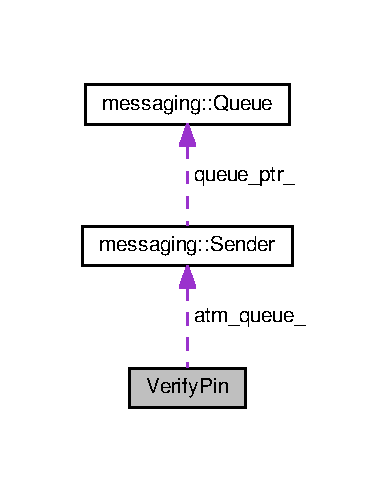
\includegraphics[width=187pt]{structVerifyPin__coll__graph}
\end{center}
\end{figure}
\subsection*{Public Member Functions}
\begin{DoxyCompactItemize}
\item 
\hyperlink{structVerifyPin_ac49a2deaf327f6582501ff5d9ea053cc}{Verify\-Pin} (const std\-::string account, const std\-::string \&pin, \hyperlink{classmessaging_1_1Sender}{messaging\-::\-Sender} atm\-\_\-queue)
\end{DoxyCompactItemize}
\subsection*{Public Attributes}
\begin{DoxyCompactItemize}
\item 
std\-::string \hyperlink{structVerifyPin_a0b4159b0183995de748fd55840e2de33}{account\-\_\-}
\item 
std\-::string \hyperlink{structVerifyPin_a5e8e9f664be63fe55500009d1b2b5a63}{pin\-\_\-}
\item 
\hyperlink{classmessaging_1_1Sender}{messaging\-::\-Sender} \hyperlink{structVerifyPin_a20cfdc37bb37447bb3036921c6f85100}{atm\-\_\-queue\-\_\-}
\end{DoxyCompactItemize}


\subsection{Constructor \& Destructor Documentation}
\hypertarget{structVerifyPin_ac49a2deaf327f6582501ff5d9ea053cc}{\index{Verify\-Pin@{Verify\-Pin}!Verify\-Pin@{Verify\-Pin}}
\index{Verify\-Pin@{Verify\-Pin}!VerifyPin@{Verify\-Pin}}
\subsubsection[{Verify\-Pin}]{\setlength{\rightskip}{0pt plus 5cm}Verify\-Pin\-::\-Verify\-Pin (
\begin{DoxyParamCaption}
\item[{const std\-::string}]{account, }
\item[{const std\-::string \&}]{pin, }
\item[{{\bf messaging\-::\-Sender}}]{atm\-\_\-queue}
\end{DoxyParamCaption}
)\hspace{0.3cm}{\ttfamily [inline]}}}\label{structVerifyPin_ac49a2deaf327f6582501ff5d9ea053cc}


\subsection{Member Data Documentation}
\hypertarget{structVerifyPin_a0b4159b0183995de748fd55840e2de33}{\index{Verify\-Pin@{Verify\-Pin}!account\-\_\-@{account\-\_\-}}
\index{account\-\_\-@{account\-\_\-}!VerifyPin@{Verify\-Pin}}
\subsubsection[{account\-\_\-}]{\setlength{\rightskip}{0pt plus 5cm}std\-::string Verify\-Pin\-::account\-\_\-}}\label{structVerifyPin_a0b4159b0183995de748fd55840e2de33}
\hypertarget{structVerifyPin_a20cfdc37bb37447bb3036921c6f85100}{\index{Verify\-Pin@{Verify\-Pin}!atm\-\_\-queue\-\_\-@{atm\-\_\-queue\-\_\-}}
\index{atm\-\_\-queue\-\_\-@{atm\-\_\-queue\-\_\-}!VerifyPin@{Verify\-Pin}}
\subsubsection[{atm\-\_\-queue\-\_\-}]{\setlength{\rightskip}{0pt plus 5cm}{\bf messaging\-::\-Sender} Verify\-Pin\-::atm\-\_\-queue\-\_\-\hspace{0.3cm}{\ttfamily [mutable]}}}\label{structVerifyPin_a20cfdc37bb37447bb3036921c6f85100}
\hypertarget{structVerifyPin_a5e8e9f664be63fe55500009d1b2b5a63}{\index{Verify\-Pin@{Verify\-Pin}!pin\-\_\-@{pin\-\_\-}}
\index{pin\-\_\-@{pin\-\_\-}!VerifyPin@{Verify\-Pin}}
\subsubsection[{pin\-\_\-}]{\setlength{\rightskip}{0pt plus 5cm}std\-::string Verify\-Pin\-::pin\-\_\-}}\label{structVerifyPin_a5e8e9f664be63fe55500009d1b2b5a63}


The documentation for this struct was generated from the following file\-:\begin{DoxyCompactItemize}
\item 
/root/\-Public/shack/atm/\hyperlink{withdraw_8h}{withdraw.\-h}\end{DoxyCompactItemize}

\hypertarget{structWithdraw}{\section{Withdraw Struct Reference}
\label{structWithdraw}\index{Withdraw@{Withdraw}}
}


{\ttfamily \#include $<$withdraw.\-h$>$}



Collaboration diagram for Withdraw\-:
\nopagebreak
\begin{figure}[H]
\begin{center}
\leavevmode
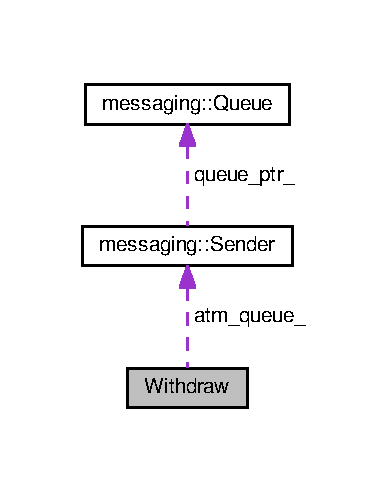
\includegraphics[width=187pt]{structWithdraw__coll__graph}
\end{center}
\end{figure}
\subsection*{Public Member Functions}
\begin{DoxyCompactItemize}
\item 
\hyperlink{structWithdraw_af748f757c832cbf3dad2cc8f050a9826}{Withdraw} (const std\-::string \&account, unsigned amount, \hyperlink{classmessaging_1_1Sender}{messaging\-::\-Sender} atm\-\_\-queue)
\end{DoxyCompactItemize}
\subsection*{Public Attributes}
\begin{DoxyCompactItemize}
\item 
std\-::string \hyperlink{structWithdraw_a3dcbc9569c0540c6d5fce8923a9c6109}{account\-\_\-}
\item 
unsigned \hyperlink{structWithdraw_aef16f3caa8a813007062a23d06ee4297}{amount\-\_\-}
\item 
\hyperlink{classmessaging_1_1Sender}{messaging\-::\-Sender} \hyperlink{structWithdraw_ab629acf79446ce7dd973ed3c97c1c99c}{atm\-\_\-queue\-\_\-}
\end{DoxyCompactItemize}


\subsection{Constructor \& Destructor Documentation}
\hypertarget{structWithdraw_af748f757c832cbf3dad2cc8f050a9826}{\index{Withdraw@{Withdraw}!Withdraw@{Withdraw}}
\index{Withdraw@{Withdraw}!Withdraw@{Withdraw}}
\subsubsection[{Withdraw}]{\setlength{\rightskip}{0pt plus 5cm}Withdraw\-::\-Withdraw (
\begin{DoxyParamCaption}
\item[{const std\-::string \&}]{account, }
\item[{unsigned}]{amount, }
\item[{{\bf messaging\-::\-Sender}}]{atm\-\_\-queue}
\end{DoxyParamCaption}
)\hspace{0.3cm}{\ttfamily [inline]}}}\label{structWithdraw_af748f757c832cbf3dad2cc8f050a9826}


\subsection{Member Data Documentation}
\hypertarget{structWithdraw_a3dcbc9569c0540c6d5fce8923a9c6109}{\index{Withdraw@{Withdraw}!account\-\_\-@{account\-\_\-}}
\index{account\-\_\-@{account\-\_\-}!Withdraw@{Withdraw}}
\subsubsection[{account\-\_\-}]{\setlength{\rightskip}{0pt plus 5cm}std\-::string Withdraw\-::account\-\_\-}}\label{structWithdraw_a3dcbc9569c0540c6d5fce8923a9c6109}
\hypertarget{structWithdraw_aef16f3caa8a813007062a23d06ee4297}{\index{Withdraw@{Withdraw}!amount\-\_\-@{amount\-\_\-}}
\index{amount\-\_\-@{amount\-\_\-}!Withdraw@{Withdraw}}
\subsubsection[{amount\-\_\-}]{\setlength{\rightskip}{0pt plus 5cm}unsigned Withdraw\-::amount\-\_\-}}\label{structWithdraw_aef16f3caa8a813007062a23d06ee4297}
\hypertarget{structWithdraw_ab629acf79446ce7dd973ed3c97c1c99c}{\index{Withdraw@{Withdraw}!atm\-\_\-queue\-\_\-@{atm\-\_\-queue\-\_\-}}
\index{atm\-\_\-queue\-\_\-@{atm\-\_\-queue\-\_\-}!Withdraw@{Withdraw}}
\subsubsection[{atm\-\_\-queue\-\_\-}]{\setlength{\rightskip}{0pt plus 5cm}{\bf messaging\-::\-Sender} Withdraw\-::atm\-\_\-queue\-\_\-\hspace{0.3cm}{\ttfamily [mutable]}}}\label{structWithdraw_ab629acf79446ce7dd973ed3c97c1c99c}


The documentation for this struct was generated from the following file\-:\begin{DoxyCompactItemize}
\item 
/root/\-Public/shack/atm/\hyperlink{withdraw_8h}{withdraw.\-h}\end{DoxyCompactItemize}

\hypertarget{structWithdrawDenied}{\section{Withdraw\-Denied Struct Reference}
\label{structWithdrawDenied}\index{Withdraw\-Denied@{Withdraw\-Denied}}
}


{\ttfamily \#include $<$withdraw.\-h$>$}



The documentation for this struct was generated from the following file\-:\begin{DoxyCompactItemize}
\item 
/root/\-Public/shack/atm/\hyperlink{withdraw_8h}{withdraw.\-h}\end{DoxyCompactItemize}

\hypertarget{structWithdrawOK}{\section{Withdraw\-O\-K Struct Reference}
\label{structWithdrawOK}\index{Withdraw\-O\-K@{Withdraw\-O\-K}}
}


{\ttfamily \#include $<$withdraw.\-h$>$}



The documentation for this struct was generated from the following file\-:\begin{DoxyCompactItemize}
\item 
/root/\-Public/shack/atm/\hyperlink{withdraw_8h}{withdraw.\-h}\end{DoxyCompactItemize}

\hypertarget{structWithdrawPressed}{\section{Withdraw\-Pressed Struct Reference}
\label{structWithdrawPressed}\index{Withdraw\-Pressed@{Withdraw\-Pressed}}
}


{\ttfamily \#include $<$withdraw.\-h$>$}

\subsection*{Public Member Functions}
\begin{DoxyCompactItemize}
\item 
\hyperlink{structWithdrawPressed_a10f3534e069eca23e8ddffe58c34faf6}{Withdraw\-Pressed} (unsigned amount)
\end{DoxyCompactItemize}
\subsection*{Public Attributes}
\begin{DoxyCompactItemize}
\item 
unsigned \hyperlink{structWithdrawPressed_ab812bf1504edd7e606dc5fa6b52f6f46}{amount\-\_\-}
\end{DoxyCompactItemize}


\subsection{Constructor \& Destructor Documentation}
\hypertarget{structWithdrawPressed_a10f3534e069eca23e8ddffe58c34faf6}{\index{Withdraw\-Pressed@{Withdraw\-Pressed}!Withdraw\-Pressed@{Withdraw\-Pressed}}
\index{Withdraw\-Pressed@{Withdraw\-Pressed}!WithdrawPressed@{Withdraw\-Pressed}}
\subsubsection[{Withdraw\-Pressed}]{\setlength{\rightskip}{0pt plus 5cm}Withdraw\-Pressed\-::\-Withdraw\-Pressed (
\begin{DoxyParamCaption}
\item[{unsigned}]{amount}
\end{DoxyParamCaption}
)\hspace{0.3cm}{\ttfamily [inline]}, {\ttfamily [explicit]}}}\label{structWithdrawPressed_a10f3534e069eca23e8ddffe58c34faf6}


\subsection{Member Data Documentation}
\hypertarget{structWithdrawPressed_ab812bf1504edd7e606dc5fa6b52f6f46}{\index{Withdraw\-Pressed@{Withdraw\-Pressed}!amount\-\_\-@{amount\-\_\-}}
\index{amount\-\_\-@{amount\-\_\-}!WithdrawPressed@{Withdraw\-Pressed}}
\subsubsection[{amount\-\_\-}]{\setlength{\rightskip}{0pt plus 5cm}unsigned Withdraw\-Pressed\-::amount\-\_\-}}\label{structWithdrawPressed_ab812bf1504edd7e606dc5fa6b52f6f46}


The documentation for this struct was generated from the following file\-:\begin{DoxyCompactItemize}
\item 
/root/\-Public/shack/atm/\hyperlink{withdraw_8h}{withdraw.\-h}\end{DoxyCompactItemize}

\hypertarget{structWithdrawProcessed}{\section{Withdraw\-Processed Struct Reference}
\label{structWithdrawProcessed}\index{Withdraw\-Processed@{Withdraw\-Processed}}
}


{\ttfamily \#include $<$withdraw.\-h$>$}

\subsection*{Public Member Functions}
\begin{DoxyCompactItemize}
\item 
\hyperlink{structWithdrawProcessed_aeb8e5c4e04a0c3abf6071bac464115b8}{Withdraw\-Processed} (const std\-::string account, unsigned amount)
\end{DoxyCompactItemize}
\subsection*{Public Attributes}
\begin{DoxyCompactItemize}
\item 
std\-::string \hyperlink{structWithdrawProcessed_afa3ac4805902cdbc81215c07d004fe38}{account\-\_\-}
\item 
unsigned \hyperlink{structWithdrawProcessed_ad80c4901e941fb58a74c1b116abcf467}{amount\-\_\-}
\end{DoxyCompactItemize}


\subsection{Constructor \& Destructor Documentation}
\hypertarget{structWithdrawProcessed_aeb8e5c4e04a0c3abf6071bac464115b8}{\index{Withdraw\-Processed@{Withdraw\-Processed}!Withdraw\-Processed@{Withdraw\-Processed}}
\index{Withdraw\-Processed@{Withdraw\-Processed}!WithdrawProcessed@{Withdraw\-Processed}}
\subsubsection[{Withdraw\-Processed}]{\setlength{\rightskip}{0pt plus 5cm}Withdraw\-Processed\-::\-Withdraw\-Processed (
\begin{DoxyParamCaption}
\item[{const std\-::string}]{account, }
\item[{unsigned}]{amount}
\end{DoxyParamCaption}
)\hspace{0.3cm}{\ttfamily [inline]}}}\label{structWithdrawProcessed_aeb8e5c4e04a0c3abf6071bac464115b8}


\subsection{Member Data Documentation}
\hypertarget{structWithdrawProcessed_afa3ac4805902cdbc81215c07d004fe38}{\index{Withdraw\-Processed@{Withdraw\-Processed}!account\-\_\-@{account\-\_\-}}
\index{account\-\_\-@{account\-\_\-}!WithdrawProcessed@{Withdraw\-Processed}}
\subsubsection[{account\-\_\-}]{\setlength{\rightskip}{0pt plus 5cm}std\-::string Withdraw\-Processed\-::account\-\_\-}}\label{structWithdrawProcessed_afa3ac4805902cdbc81215c07d004fe38}
\hypertarget{structWithdrawProcessed_ad80c4901e941fb58a74c1b116abcf467}{\index{Withdraw\-Processed@{Withdraw\-Processed}!amount\-\_\-@{amount\-\_\-}}
\index{amount\-\_\-@{amount\-\_\-}!WithdrawProcessed@{Withdraw\-Processed}}
\subsubsection[{amount\-\_\-}]{\setlength{\rightskip}{0pt plus 5cm}unsigned Withdraw\-Processed\-::amount\-\_\-}}\label{structWithdrawProcessed_ad80c4901e941fb58a74c1b116abcf467}


The documentation for this struct was generated from the following file\-:\begin{DoxyCompactItemize}
\item 
/root/\-Public/shack/atm/\hyperlink{withdraw_8h}{withdraw.\-h}\end{DoxyCompactItemize}

\hypertarget{structmessaging_1_1WrappedMessage}{\section{messaging\-:\-:Wrapped\-Message$<$ Msg $>$ Struct Template Reference}
\label{structmessaging_1_1WrappedMessage}\index{messaging\-::\-Wrapped\-Message$<$ Msg $>$@{messaging\-::\-Wrapped\-Message$<$ Msg $>$}}
}


{\ttfamily \#include $<$queue.\-h$>$}



Inheritance diagram for messaging\-:\-:Wrapped\-Message$<$ Msg $>$\-:\nopagebreak
\begin{figure}[H]
\begin{center}
\leavevmode
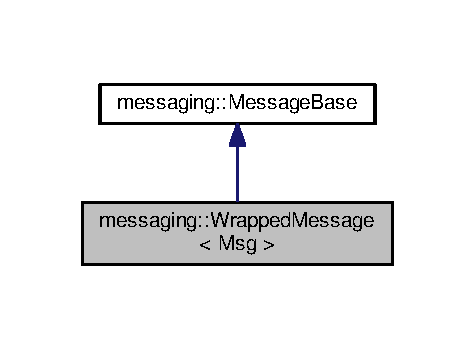
\includegraphics[width=228pt]{structmessaging_1_1WrappedMessage__inherit__graph}
\end{center}
\end{figure}


Collaboration diagram for messaging\-:\-:Wrapped\-Message$<$ Msg $>$\-:\nopagebreak
\begin{figure}[H]
\begin{center}
\leavevmode
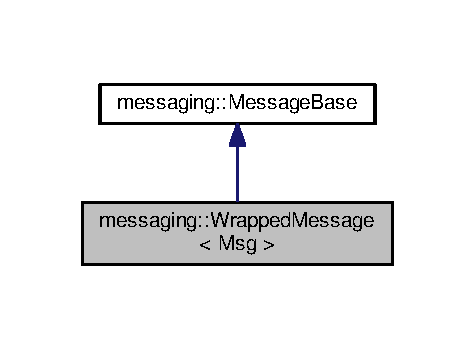
\includegraphics[width=228pt]{structmessaging_1_1WrappedMessage__coll__graph}
\end{center}
\end{figure}
\subsection*{Public Member Functions}
\begin{DoxyCompactItemize}
\item 
\hyperlink{structmessaging_1_1WrappedMessage_a1c4326bb674fcb8c82e77554618d4c46}{Wrapped\-Message} (const Msg \&contents)
\end{DoxyCompactItemize}
\subsection*{Public Attributes}
\begin{DoxyCompactItemize}
\item 
Msg \hyperlink{structmessaging_1_1WrappedMessage_a7bd8849ddcc85328985384636caa7199}{contents\-\_\-}
\end{DoxyCompactItemize}


\subsection{Constructor \& Destructor Documentation}
\hypertarget{structmessaging_1_1WrappedMessage_a1c4326bb674fcb8c82e77554618d4c46}{\index{messaging\-::\-Wrapped\-Message@{messaging\-::\-Wrapped\-Message}!Wrapped\-Message@{Wrapped\-Message}}
\index{Wrapped\-Message@{Wrapped\-Message}!messaging::WrappedMessage@{messaging\-::\-Wrapped\-Message}}
\subsubsection[{Wrapped\-Message}]{\setlength{\rightskip}{0pt plus 5cm}template$<$class Msg $>$ {\bf messaging\-::\-Wrapped\-Message}$<$ Msg $>$\-::{\bf Wrapped\-Message} (
\begin{DoxyParamCaption}
\item[{const Msg \&}]{contents}
\end{DoxyParamCaption}
)\hspace{0.3cm}{\ttfamily [inline]}, {\ttfamily [explicit]}}}\label{structmessaging_1_1WrappedMessage_a1c4326bb674fcb8c82e77554618d4c46}


\subsection{Member Data Documentation}
\hypertarget{structmessaging_1_1WrappedMessage_a7bd8849ddcc85328985384636caa7199}{\index{messaging\-::\-Wrapped\-Message@{messaging\-::\-Wrapped\-Message}!contents\-\_\-@{contents\-\_\-}}
\index{contents\-\_\-@{contents\-\_\-}!messaging::WrappedMessage@{messaging\-::\-Wrapped\-Message}}
\subsubsection[{contents\-\_\-}]{\setlength{\rightskip}{0pt plus 5cm}template$<$class Msg $>$ Msg {\bf messaging\-::\-Wrapped\-Message}$<$ Msg $>$\-::contents\-\_\-}}\label{structmessaging_1_1WrappedMessage_a7bd8849ddcc85328985384636caa7199}


The documentation for this struct was generated from the following file\-:\begin{DoxyCompactItemize}
\item 
/root/\-Public/shack/atm/\hyperlink{queue_8h}{queue.\-h}\end{DoxyCompactItemize}

\chapter{File Documentation}
\hypertarget{atm_8h}{\section{/root/\-Public/shack/atm/atm.h File Reference}
\label{atm_8h}\index{/root/\-Public/shack/atm/atm.\-h@{/root/\-Public/shack/atm/atm.\-h}}
}
{\ttfamily \#include \char`\"{}sender.\-h\char`\"{}}\\*
{\ttfamily \#include \char`\"{}receiver.\-h\char`\"{}}\\*
{\ttfamily \#include \char`\"{}withdraw.\-h\char`\"{}}\\*
{\ttfamily \#include $<$string$>$}\\*
Include dependency graph for atm.\-h\-:\nopagebreak
\begin{figure}[H]
\begin{center}
\leavevmode
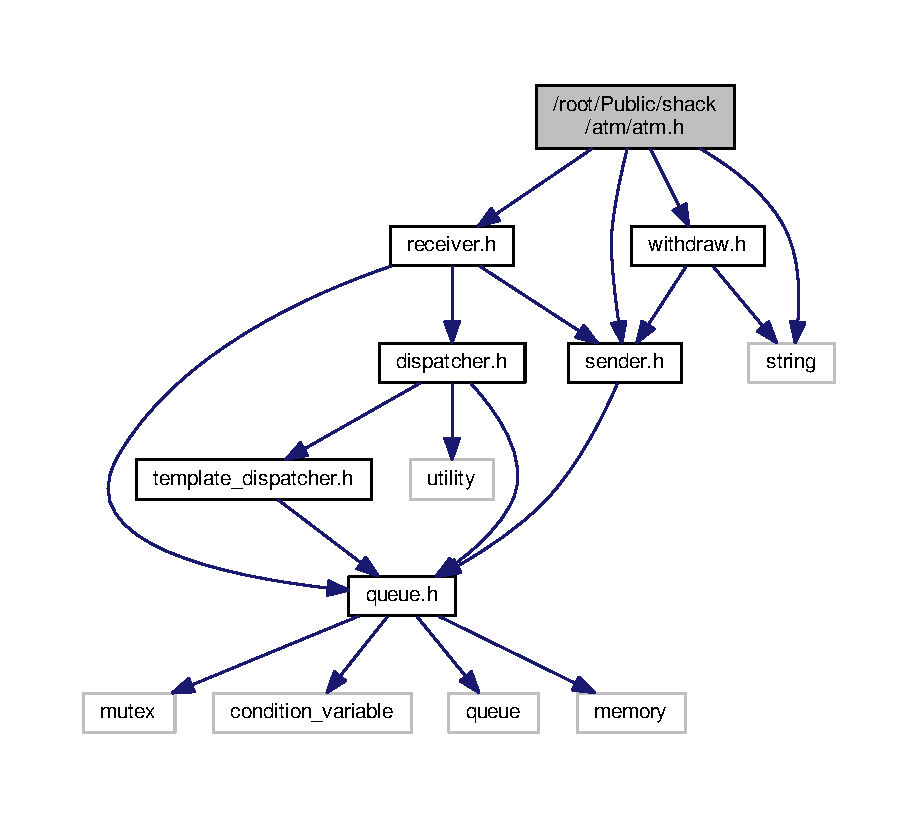
\includegraphics[width=350pt]{atm_8h__incl}
\end{center}
\end{figure}
This graph shows which files directly or indirectly include this file\-:\nopagebreak
\begin{figure}[H]
\begin{center}
\leavevmode
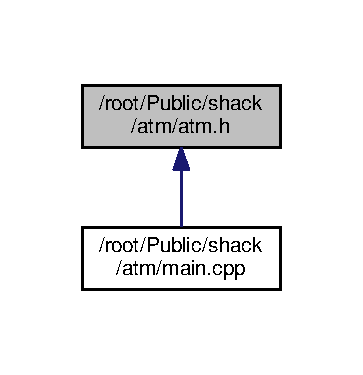
\includegraphics[width=174pt]{atm_8h__dep__incl}
\end{center}
\end{figure}
\subsection*{Classes}
\begin{DoxyCompactItemize}
\item 
class \hyperlink{classATM}{A\-T\-M}
\end{DoxyCompactItemize}

\hypertarget{atm__env_8h}{\section{/root/\-Public/shack/atm/atm\-\_\-env.h File Reference}
\label{atm__env_8h}\index{/root/\-Public/shack/atm/atm\-\_\-env.\-h@{/root/\-Public/shack/atm/atm\-\_\-env.\-h}}
}

\hypertarget{bank__machine_8h}{\section{/root/\-Public/shack/atm/bank\-\_\-machine.h File Reference}
\label{bank__machine_8h}\index{/root/\-Public/shack/atm/bank\-\_\-machine.\-h@{/root/\-Public/shack/atm/bank\-\_\-machine.\-h}}
}
{\ttfamily \#include \char`\"{}withdraw.\-h\char`\"{}}\\*
{\ttfamily \#include \char`\"{}receiver.\-h\char`\"{}}\\*
Include dependency graph for bank\-\_\-machine.\-h\-:\nopagebreak
\begin{figure}[H]
\begin{center}
\leavevmode
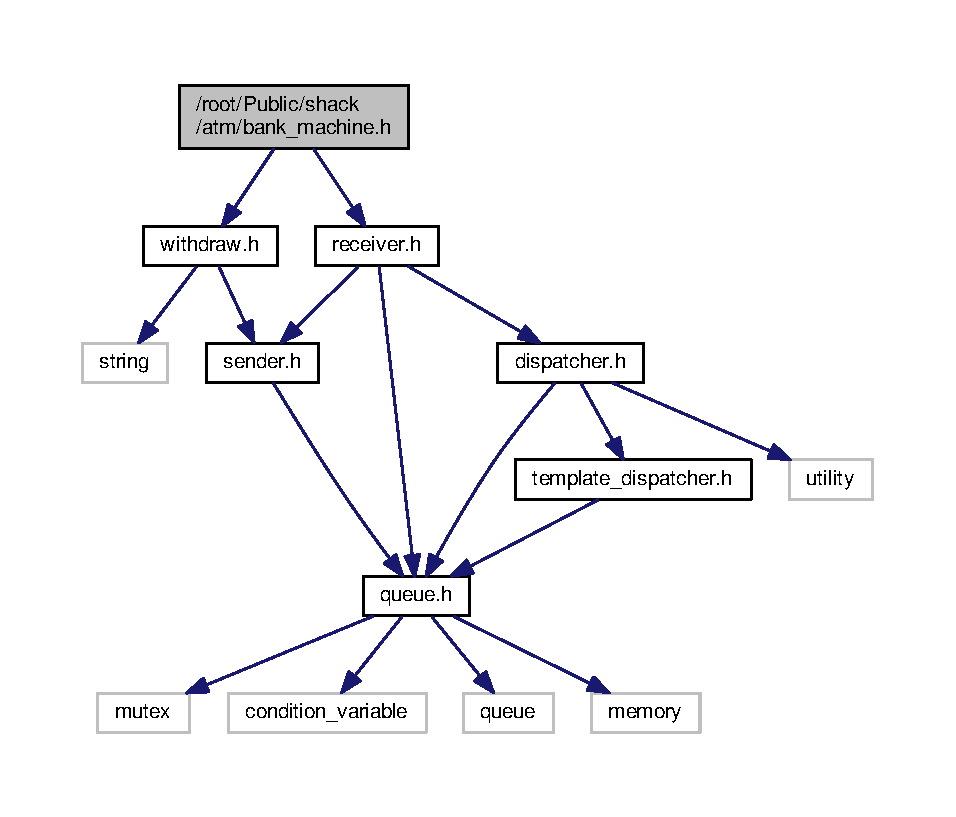
\includegraphics[width=350pt]{bank__machine_8h__incl}
\end{center}
\end{figure}
This graph shows which files directly or indirectly include this file\-:\nopagebreak
\begin{figure}[H]
\begin{center}
\leavevmode
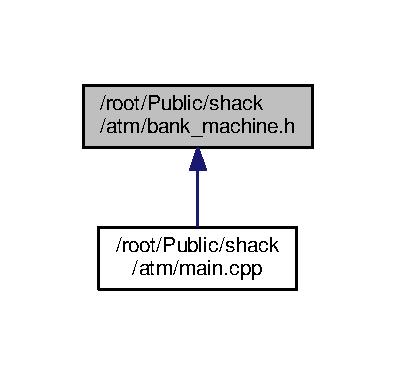
\includegraphics[width=190pt]{bank__machine_8h__dep__incl}
\end{center}
\end{figure}
\subsection*{Classes}
\begin{DoxyCompactItemize}
\item 
class \hyperlink{classBankMachine}{Bank\-Machine}
\end{DoxyCompactItemize}

\hypertarget{dispatcher_8cpp}{\section{/root/\-Public/shack/atm/dispatcher.cpp File Reference}
\label{dispatcher_8cpp}\index{/root/\-Public/shack/atm/dispatcher.\-cpp@{/root/\-Public/shack/atm/dispatcher.\-cpp}}
}
{\ttfamily \#include \char`\"{}dispatcher.\-h\char`\"{}}\\*
Include dependency graph for dispatcher.\-cpp\-:\nopagebreak
\begin{figure}[H]
\begin{center}
\leavevmode
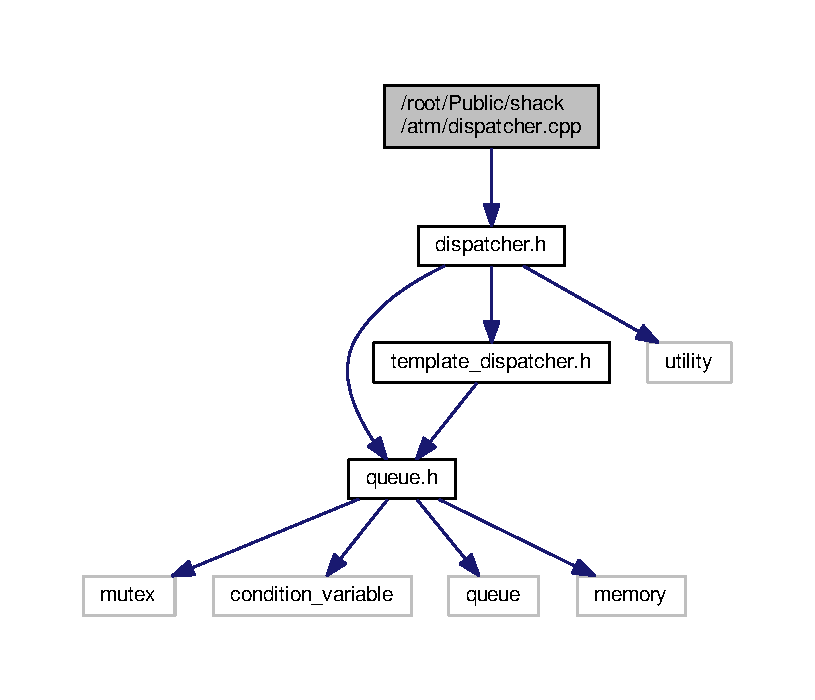
\includegraphics[width=350pt]{dispatcher_8cpp__incl}
\end{center}
\end{figure}

\hypertarget{dispatcher_8h}{\section{/root/\-Public/shack/atm/dispatcher.h File Reference}
\label{dispatcher_8h}\index{/root/\-Public/shack/atm/dispatcher.\-h@{/root/\-Public/shack/atm/dispatcher.\-h}}
}
{\ttfamily \#include \char`\"{}queue.\-h\char`\"{}}\\*
{\ttfamily \#include \char`\"{}template\-\_\-dispatcher.\-h\char`\"{}}\\*
{\ttfamily \#include $<$utility$>$}\\*
Include dependency graph for dispatcher.\-h\-:\nopagebreak
\begin{figure}[H]
\begin{center}
\leavevmode
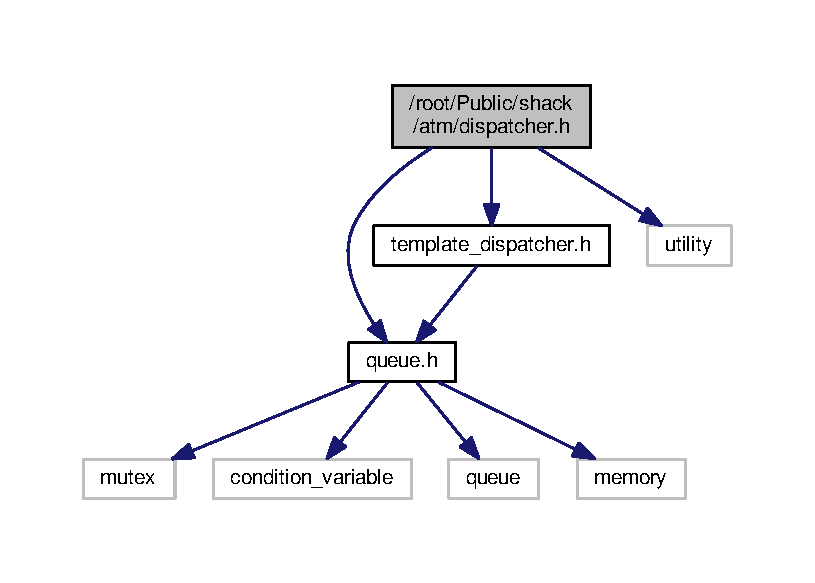
\includegraphics[width=350pt]{dispatcher_8h__incl}
\end{center}
\end{figure}
This graph shows which files directly or indirectly include this file\-:\nopagebreak
\begin{figure}[H]
\begin{center}
\leavevmode
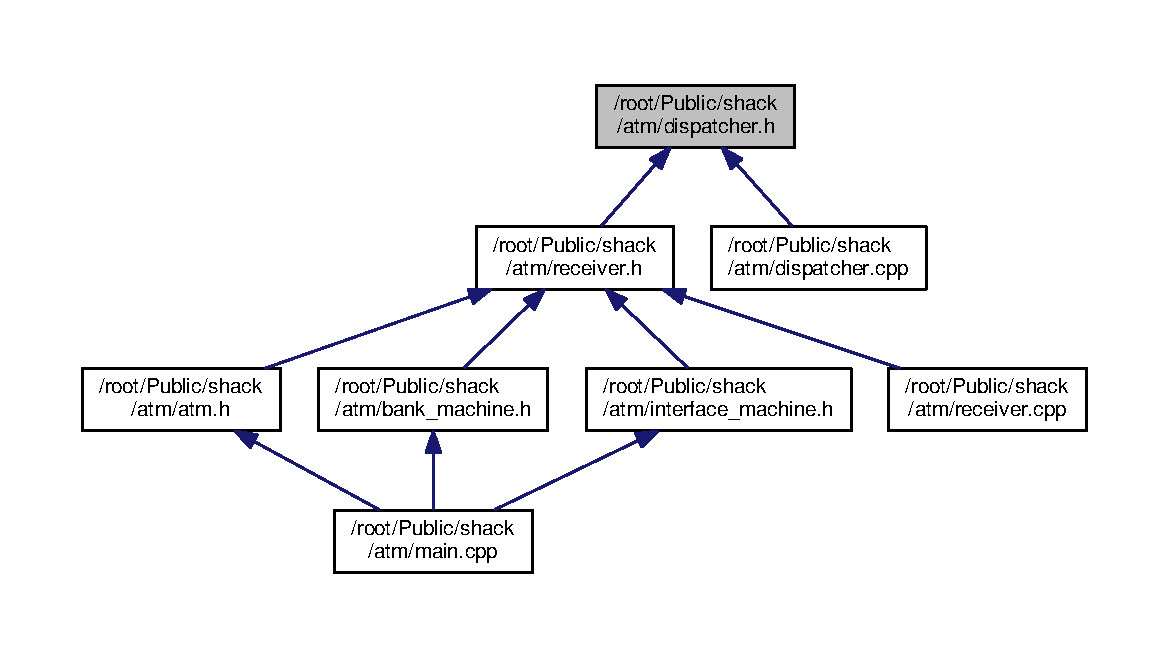
\includegraphics[width=350pt]{dispatcher_8h__dep__incl}
\end{center}
\end{figure}
\subsection*{Classes}
\begin{DoxyCompactItemize}
\item 
class \hyperlink{classmessaging_1_1CloseQueue}{messaging\-::\-Close\-Queue}
\item 
class \hyperlink{classmessaging_1_1Dispatcher}{messaging\-::\-Dispatcher}
\end{DoxyCompactItemize}
\subsection*{Namespaces}
\begin{DoxyCompactItemize}
\item 
\hyperlink{namespacemessaging}{messaging}
\end{DoxyCompactItemize}

\hypertarget{interface__machine_8h}{\section{/root/\-Public/shack/atm/interface\-\_\-machine.h File Reference}
\label{interface__machine_8h}\index{/root/\-Public/shack/atm/interface\-\_\-machine.\-h@{/root/\-Public/shack/atm/interface\-\_\-machine.\-h}}
}
{\ttfamily \#include \char`\"{}receiver.\-h\char`\"{}}\\*
{\ttfamily \#include \char`\"{}withdraw.\-h\char`\"{}}\\*
{\ttfamily \#include $<$mutex$>$}\\*
{\ttfamily \#include $<$iostream$>$}\\*
Include dependency graph for interface\-\_\-machine.\-h\-:\nopagebreak
\begin{figure}[H]
\begin{center}
\leavevmode
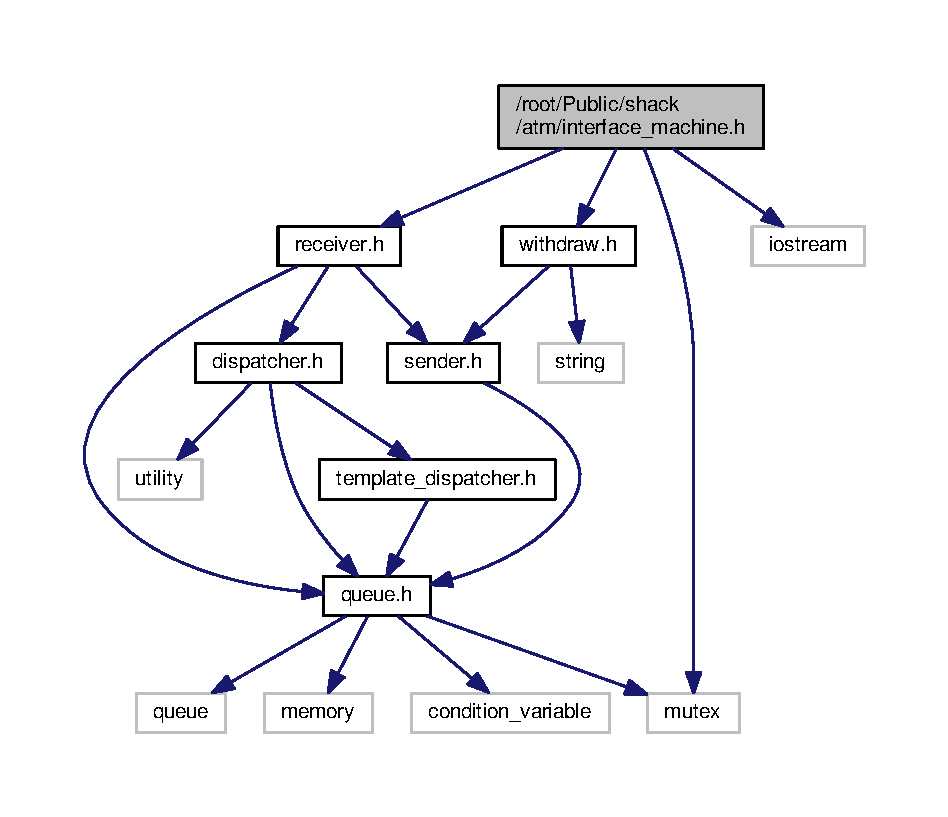
\includegraphics[width=350pt]{interface__machine_8h__incl}
\end{center}
\end{figure}
This graph shows which files directly or indirectly include this file\-:\nopagebreak
\begin{figure}[H]
\begin{center}
\leavevmode
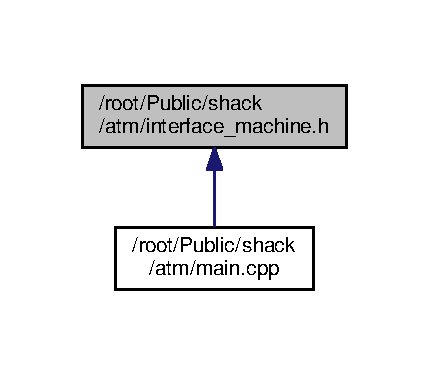
\includegraphics[width=206pt]{interface__machine_8h__dep__incl}
\end{center}
\end{figure}
\subsection*{Classes}
\begin{DoxyCompactItemize}
\item 
class \hyperlink{classInterfaceMachine}{Interface\-Machine}
\end{DoxyCompactItemize}

\hypertarget{main_8cpp}{\section{/root/\-Public/shack/atm/main.cpp File Reference}
\label{main_8cpp}\index{/root/\-Public/shack/atm/main.\-cpp@{/root/\-Public/shack/atm/main.\-cpp}}
}
{\ttfamily \#include \char`\"{}bank\-\_\-machine.\-h\char`\"{}}\\*
{\ttfamily \#include \char`\"{}interface\-\_\-machine.\-h\char`\"{}}\\*
{\ttfamily \#include \char`\"{}atm.\-h\char`\"{}}\\*
{\ttfamily \#include $<$thread$>$}\\*
{\ttfamily \#include $<$cstdio$>$}\\*
{\ttfamily \#include $<$iostream$>$}\\*
Include dependency graph for main.\-cpp\-:\nopagebreak
\begin{figure}[H]
\begin{center}
\leavevmode
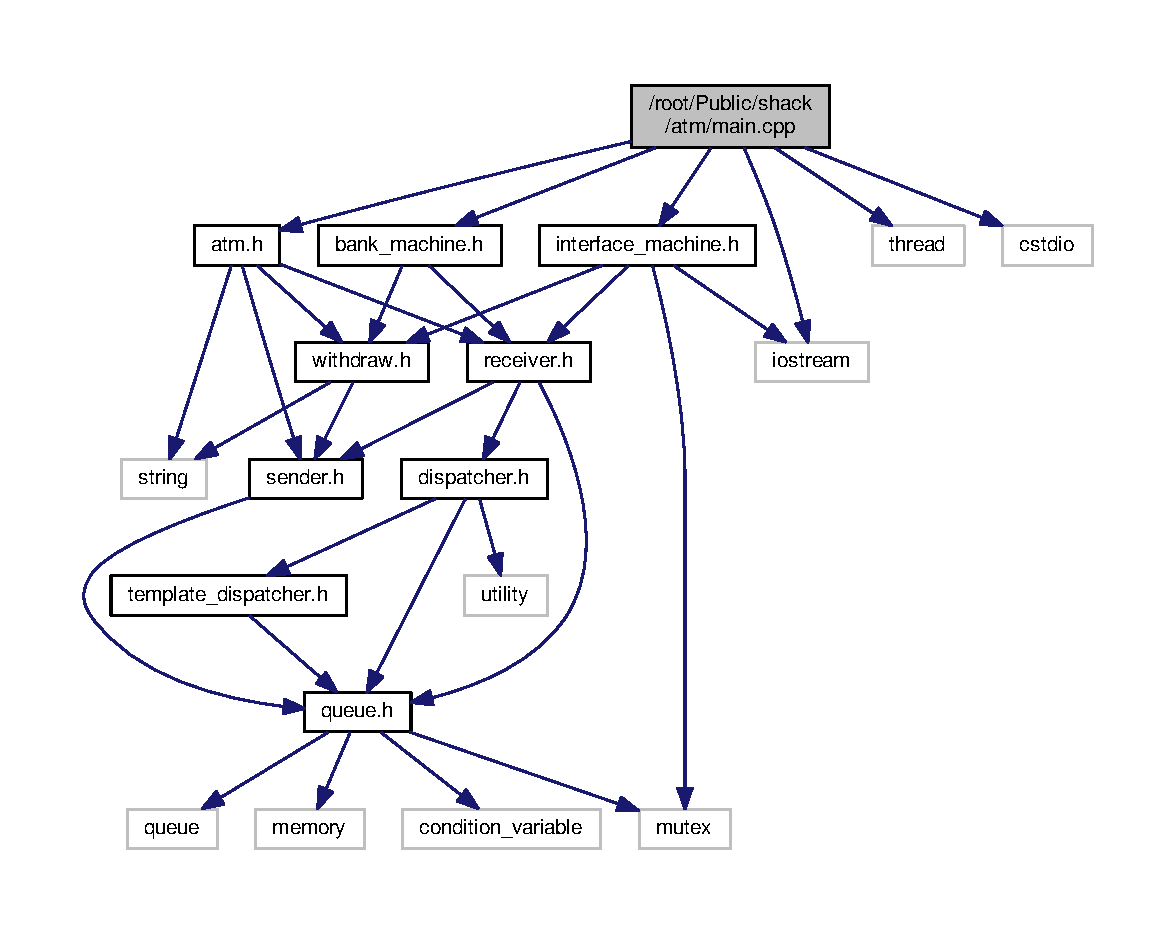
\includegraphics[width=350pt]{main_8cpp__incl}
\end{center}
\end{figure}
\subsection*{Functions}
\begin{DoxyCompactItemize}
\item 
int \hyperlink{main_8cpp_ae66f6b31b5ad750f1fe042a706a4e3d4}{main} ()
\end{DoxyCompactItemize}


\subsection{Function Documentation}
\hypertarget{main_8cpp_ae66f6b31b5ad750f1fe042a706a4e3d4}{\index{main.\-cpp@{main.\-cpp}!main@{main}}
\index{main@{main}!main.cpp@{main.\-cpp}}
\subsubsection[{main}]{\setlength{\rightskip}{0pt plus 5cm}int main (
\begin{DoxyParamCaption}
{}
\end{DoxyParamCaption}
)}}\label{main_8cpp_ae66f6b31b5ad750f1fe042a706a4e3d4}


Here is the call graph for this function\-:
\nopagebreak
\begin{figure}[H]
\begin{center}
\leavevmode
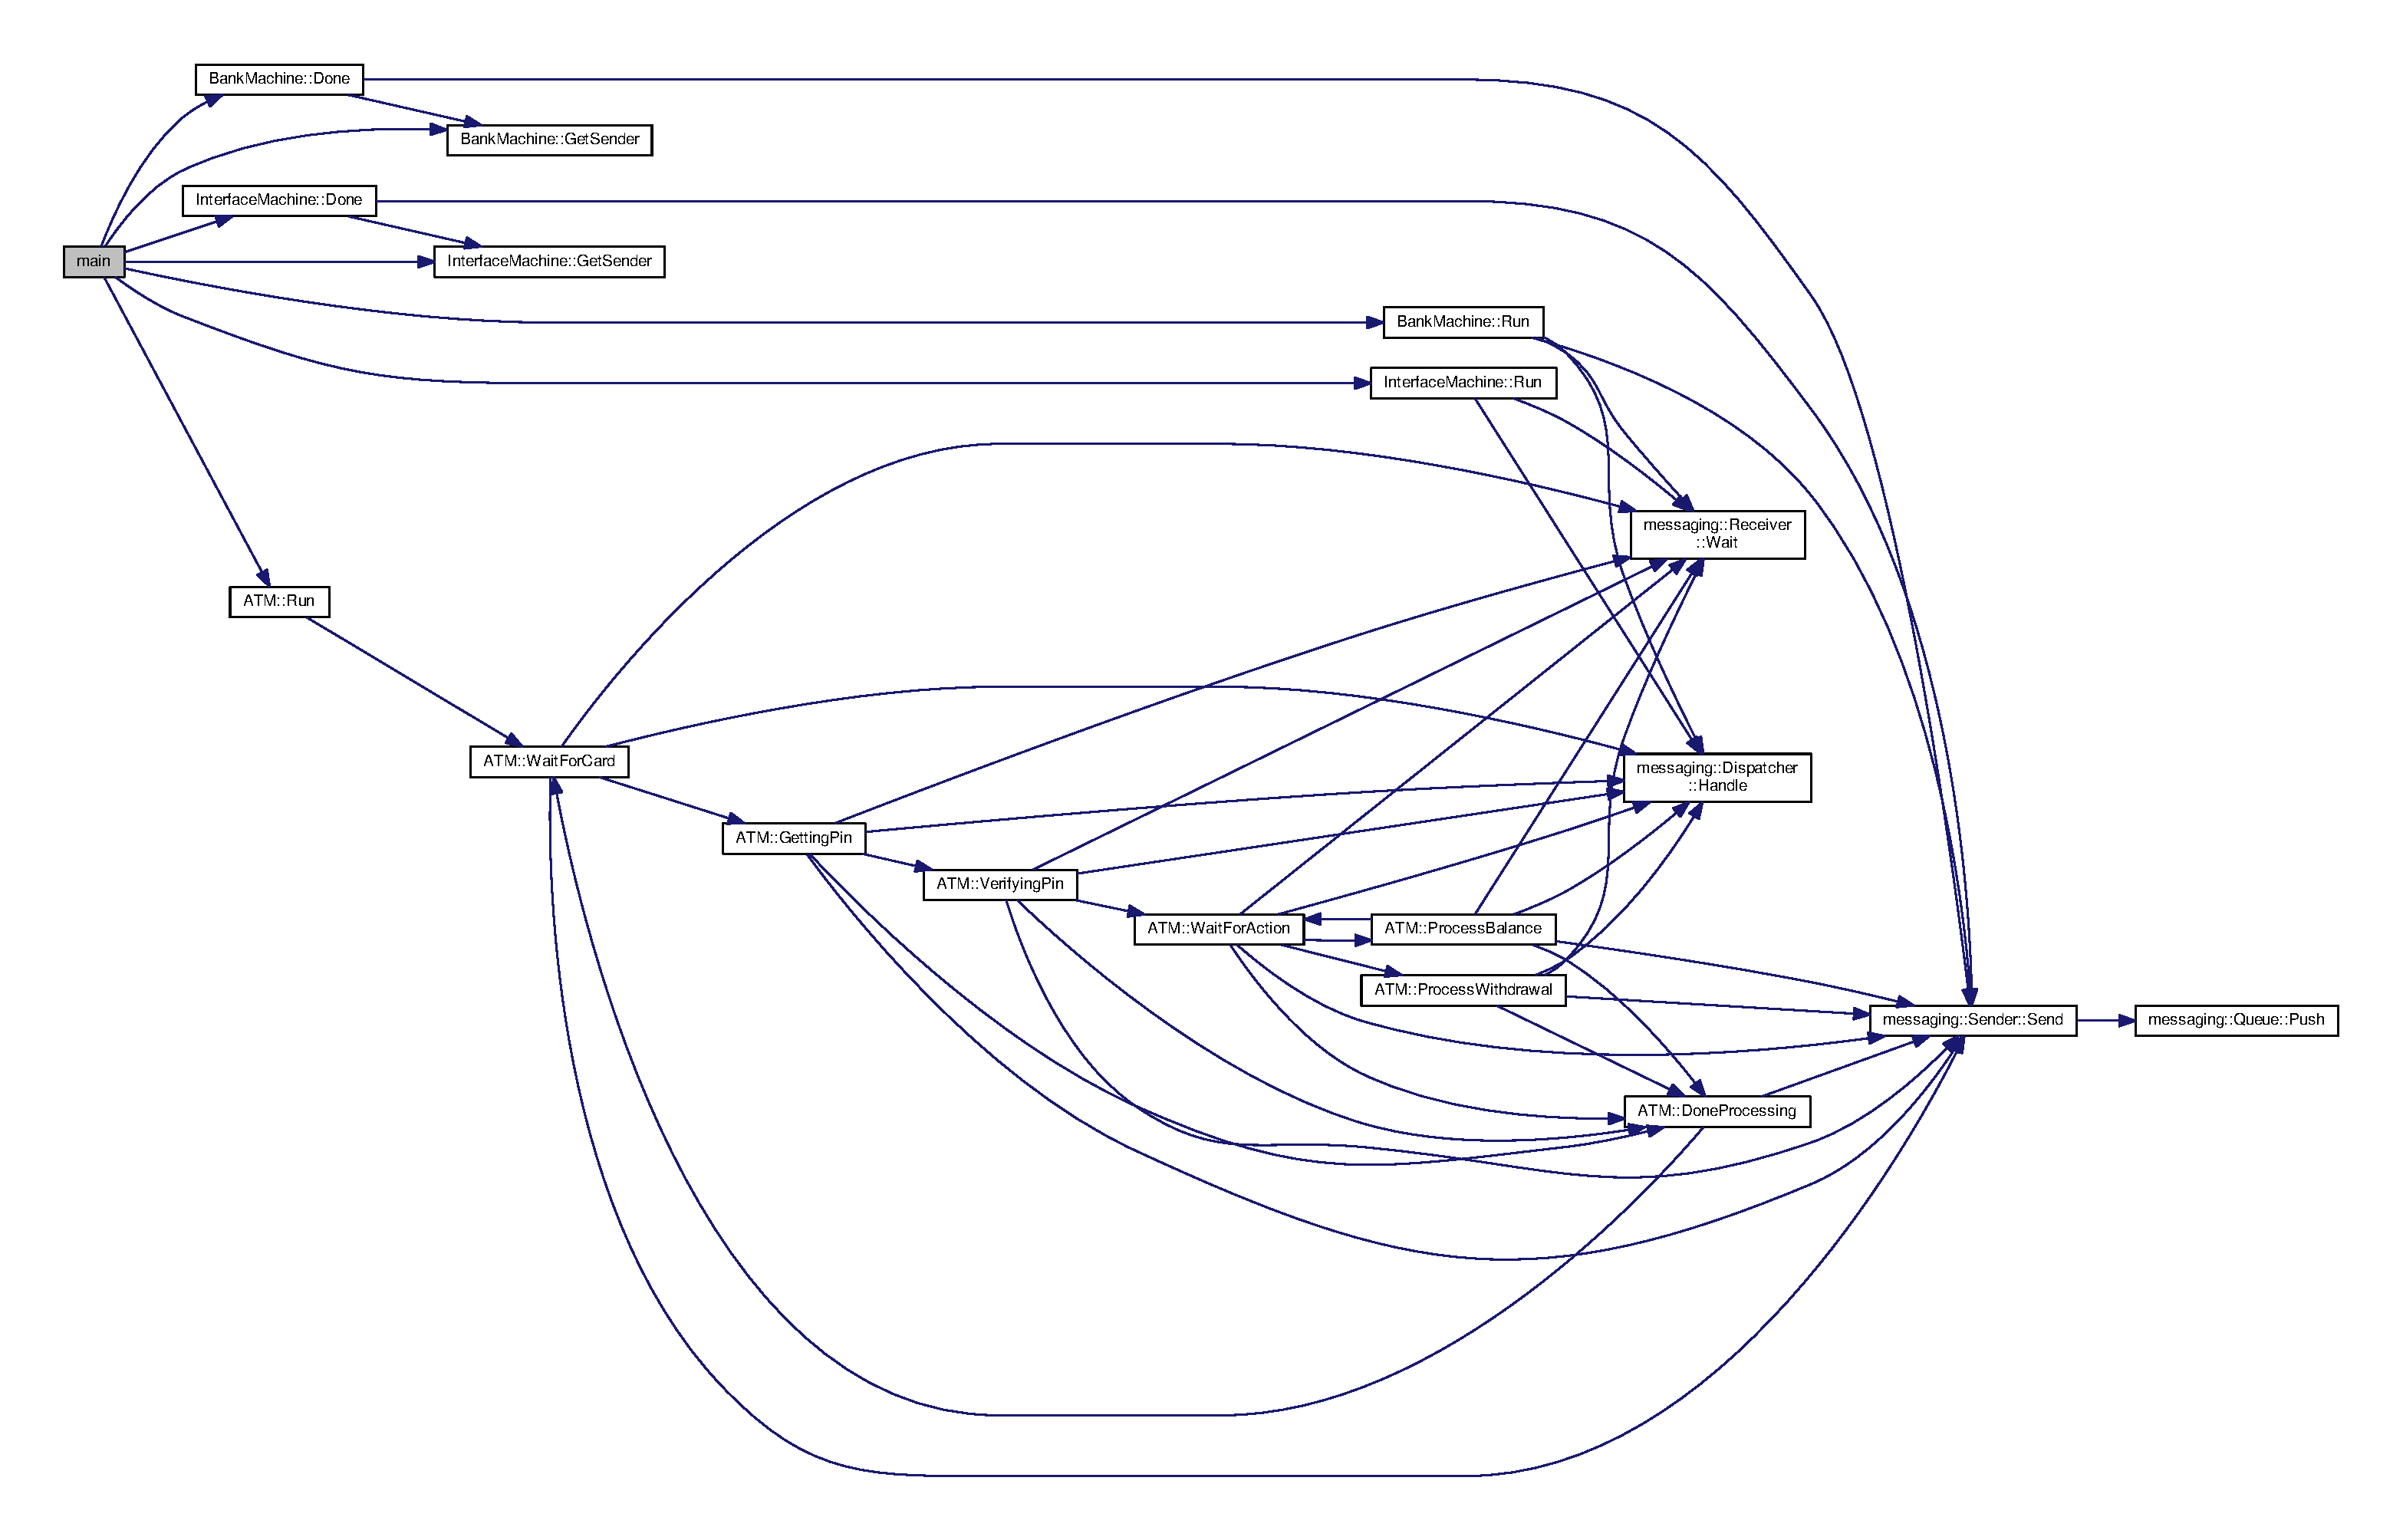
\includegraphics[width=350pt]{main_8cpp_ae66f6b31b5ad750f1fe042a706a4e3d4_cgraph}
\end{center}
\end{figure}



\hypertarget{queue_8cpp}{\section{/root/\-Public/shack/atm/queue.cpp File Reference}
\label{queue_8cpp}\index{/root/\-Public/shack/atm/queue.\-cpp@{/root/\-Public/shack/atm/queue.\-cpp}}
}
{\ttfamily \#include \char`\"{}queue.\-h\char`\"{}}\\*
Include dependency graph for queue.\-cpp\-:\nopagebreak
\begin{figure}[H]
\begin{center}
\leavevmode
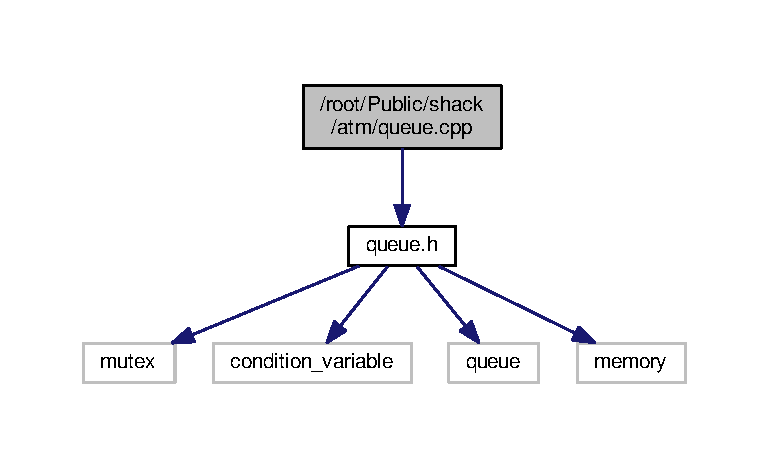
\includegraphics[width=350pt]{queue_8cpp__incl}
\end{center}
\end{figure}

\hypertarget{queue_8h}{\section{/root/\-Public/shack/atm/queue.h File Reference}
\label{queue_8h}\index{/root/\-Public/shack/atm/queue.\-h@{/root/\-Public/shack/atm/queue.\-h}}
}
{\ttfamily \#include $<$mutex$>$}\\*
{\ttfamily \#include $<$condition\-\_\-variable$>$}\\*
{\ttfamily \#include $<$queue$>$}\\*
{\ttfamily \#include $<$memory$>$}\\*
Include dependency graph for queue.\-h\-:\nopagebreak
\begin{figure}[H]
\begin{center}
\leavevmode
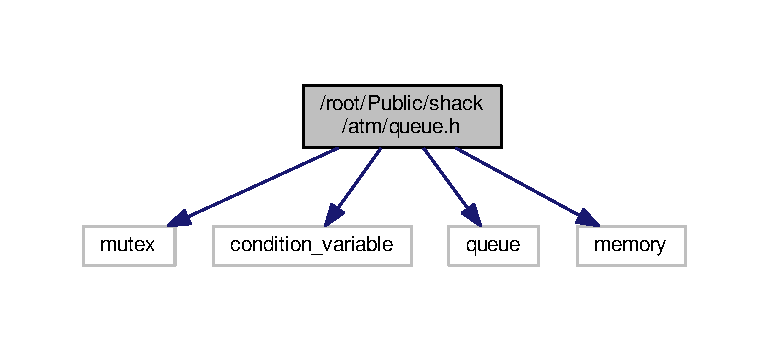
\includegraphics[width=350pt]{queue_8h__incl}
\end{center}
\end{figure}
This graph shows which files directly or indirectly include this file\-:\nopagebreak
\begin{figure}[H]
\begin{center}
\leavevmode
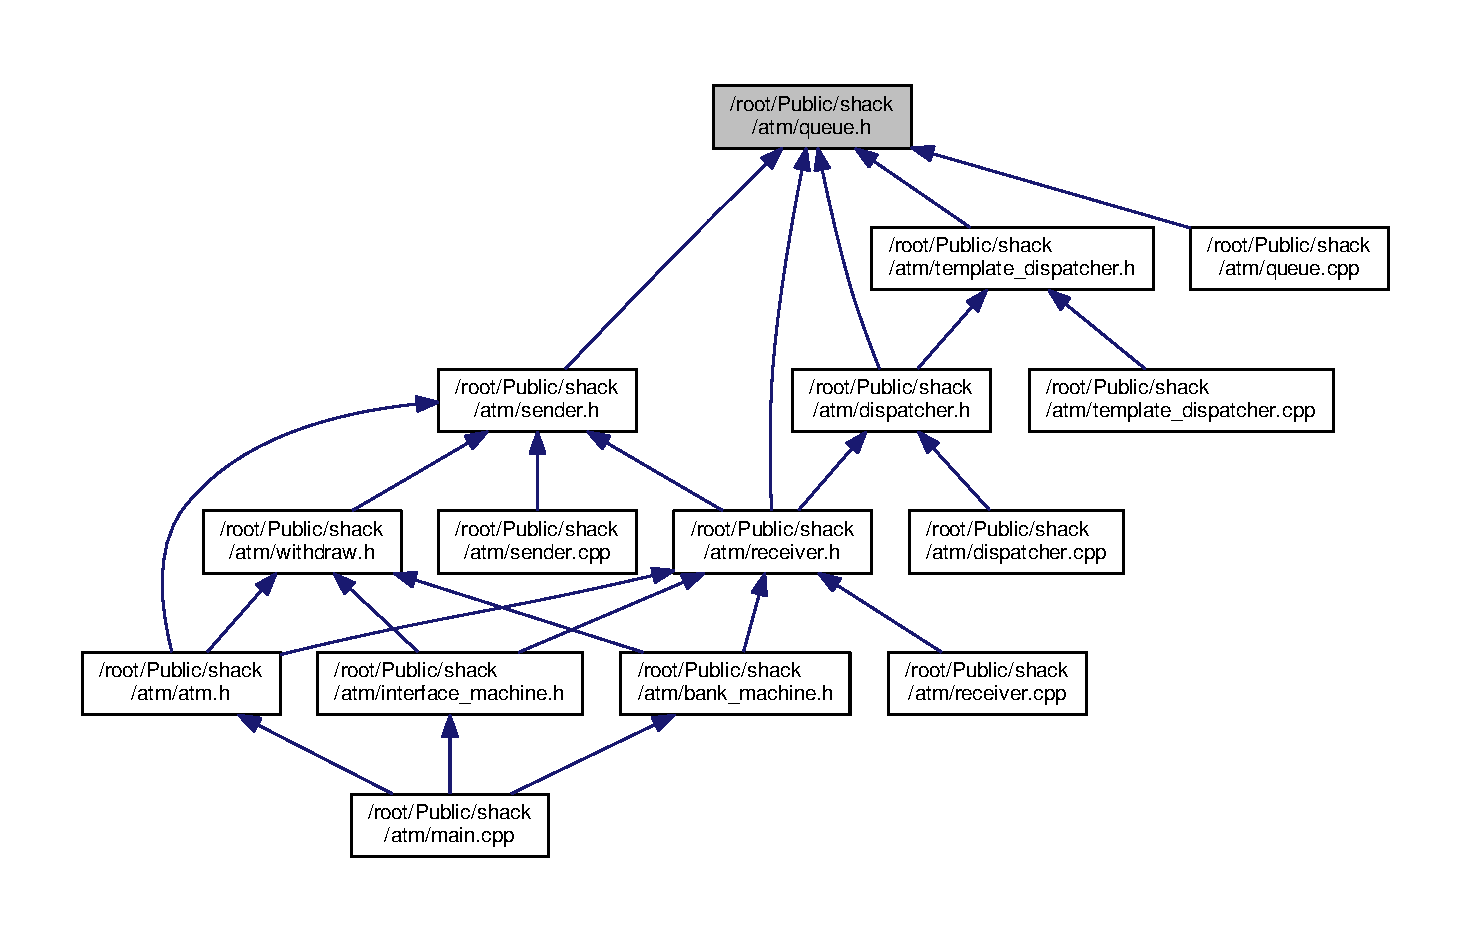
\includegraphics[width=350pt]{queue_8h__dep__incl}
\end{center}
\end{figure}
\subsection*{Classes}
\begin{DoxyCompactItemize}
\item 
struct \hyperlink{structmessaging_1_1MessageBase}{messaging\-::\-Message\-Base}
\item 
struct \hyperlink{structmessaging_1_1WrappedMessage}{messaging\-::\-Wrapped\-Message$<$ Msg $>$}
\item 
class \hyperlink{classmessaging_1_1Queue}{messaging\-::\-Queue}
\end{DoxyCompactItemize}
\subsection*{Namespaces}
\begin{DoxyCompactItemize}
\item 
\hyperlink{namespacemessaging}{messaging}
\end{DoxyCompactItemize}

\hypertarget{receiver_8cpp}{\section{/root/\-Public/shack/atm/receiver.cpp File Reference}
\label{receiver_8cpp}\index{/root/\-Public/shack/atm/receiver.\-cpp@{/root/\-Public/shack/atm/receiver.\-cpp}}
}
{\ttfamily \#include \char`\"{}receiver.\-h\char`\"{}}\\*
Include dependency graph for receiver.\-cpp\-:\nopagebreak
\begin{figure}[H]
\begin{center}
\leavevmode
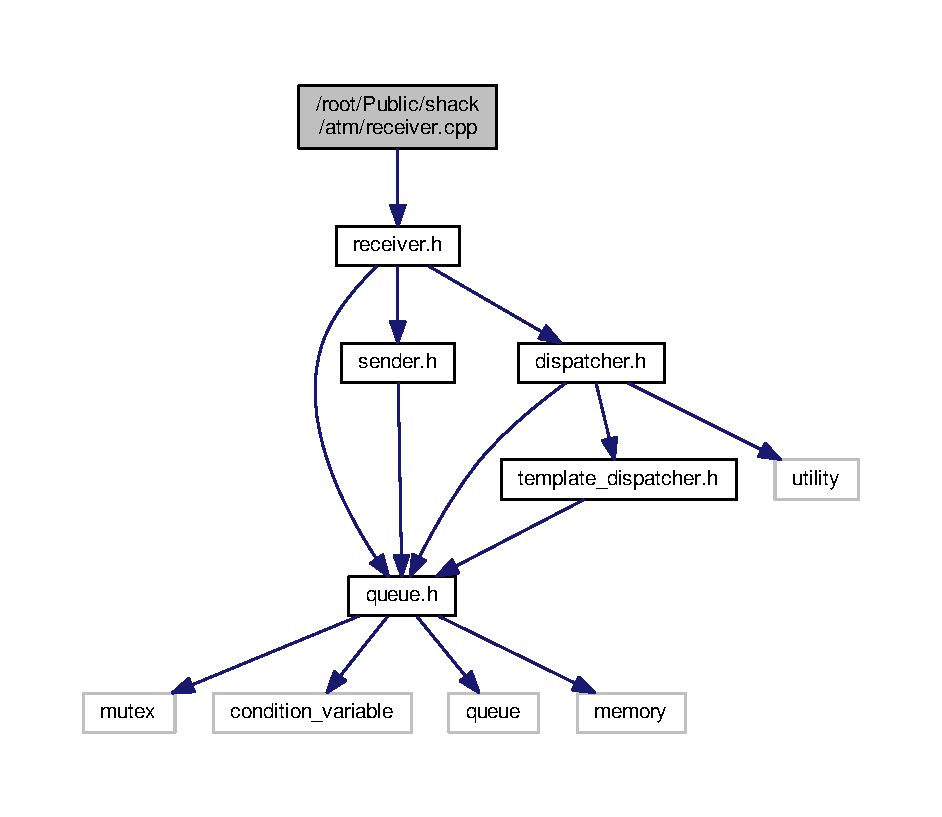
\includegraphics[width=350pt]{receiver_8cpp__incl}
\end{center}
\end{figure}

\hypertarget{receiver_8h}{\section{/root/\-Public/shack/atm/receiver.h File Reference}
\label{receiver_8h}\index{/root/\-Public/shack/atm/receiver.\-h@{/root/\-Public/shack/atm/receiver.\-h}}
}
{\ttfamily \#include \char`\"{}queue.\-h\char`\"{}}\\*
{\ttfamily \#include \char`\"{}sender.\-h\char`\"{}}\\*
{\ttfamily \#include \char`\"{}dispatcher.\-h\char`\"{}}\\*
Include dependency graph for receiver.\-h\-:\nopagebreak
\begin{figure}[H]
\begin{center}
\leavevmode
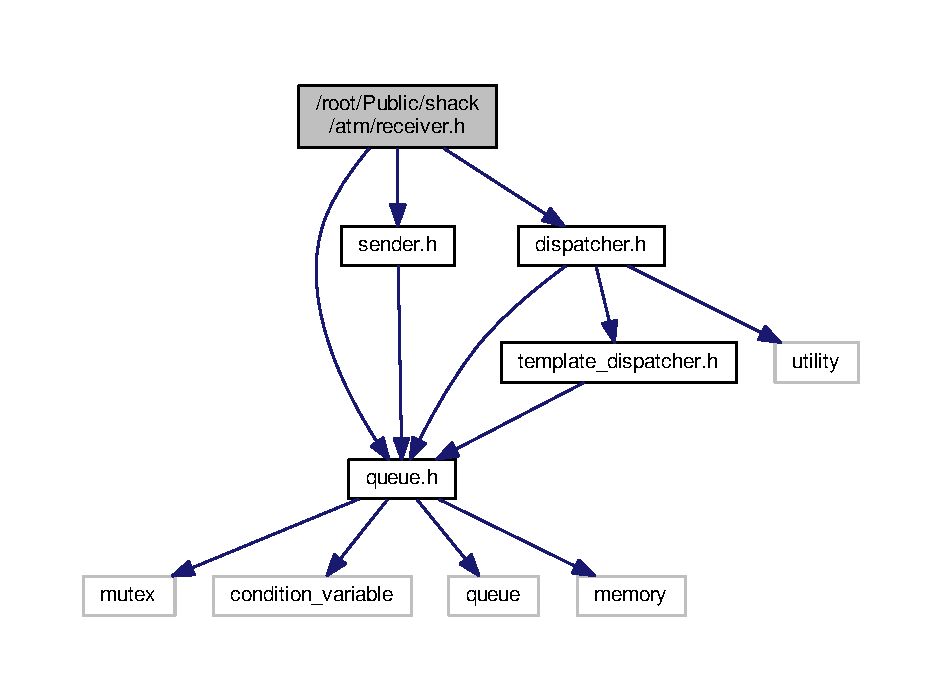
\includegraphics[width=350pt]{receiver_8h__incl}
\end{center}
\end{figure}
This graph shows which files directly or indirectly include this file\-:\nopagebreak
\begin{figure}[H]
\begin{center}
\leavevmode
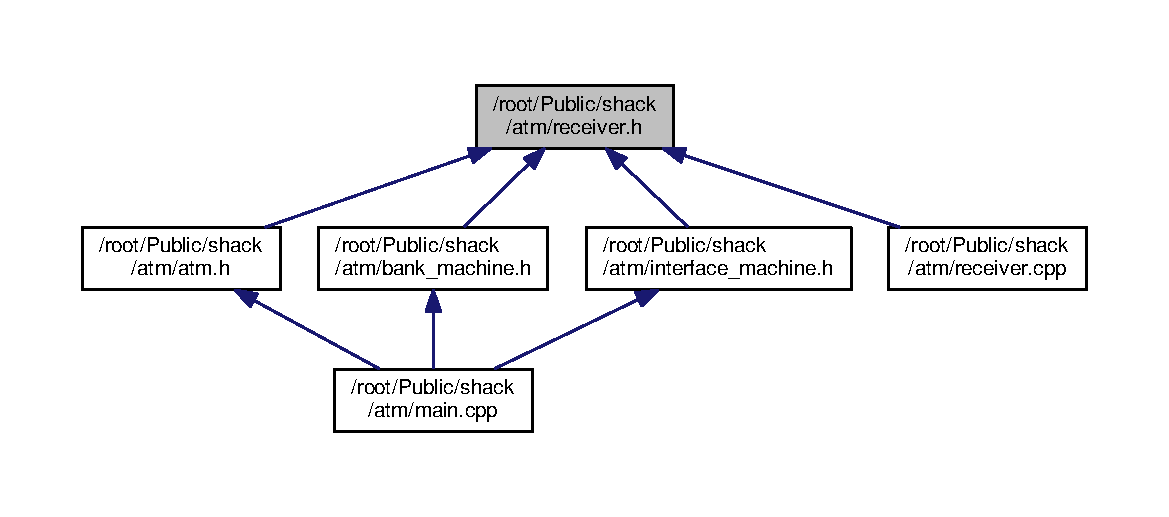
\includegraphics[width=350pt]{receiver_8h__dep__incl}
\end{center}
\end{figure}
\subsection*{Classes}
\begin{DoxyCompactItemize}
\item 
class \hyperlink{classmessaging_1_1Receiver}{messaging\-::\-Receiver}
\end{DoxyCompactItemize}
\subsection*{Namespaces}
\begin{DoxyCompactItemize}
\item 
\hyperlink{namespacemessaging}{messaging}
\end{DoxyCompactItemize}

\hypertarget{sender_8cpp}{\section{/root/\-Public/shack/atm/sender.cpp File Reference}
\label{sender_8cpp}\index{/root/\-Public/shack/atm/sender.\-cpp@{/root/\-Public/shack/atm/sender.\-cpp}}
}
{\ttfamily \#include \char`\"{}sender.\-h\char`\"{}}\\*
Include dependency graph for sender.\-cpp\-:\nopagebreak
\begin{figure}[H]
\begin{center}
\leavevmode
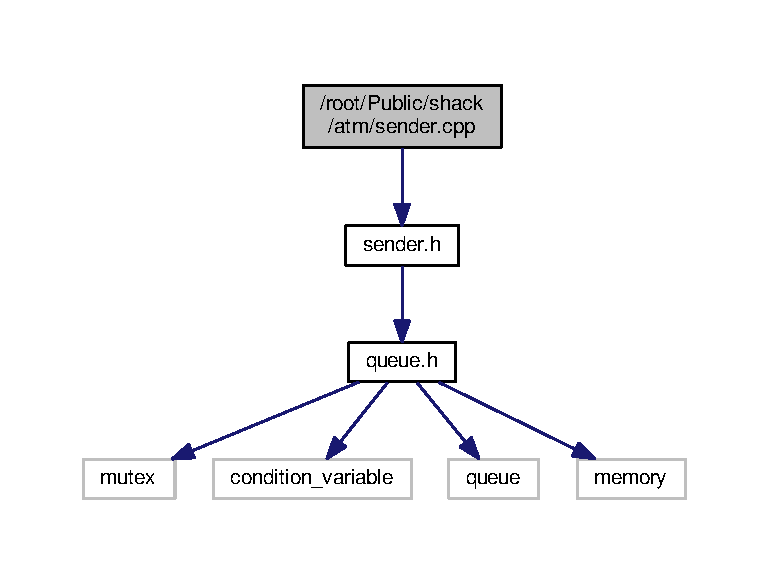
\includegraphics[width=350pt]{sender_8cpp__incl}
\end{center}
\end{figure}

\hypertarget{sender_8h}{\section{/root/\-Public/shack/atm/sender.h File Reference}
\label{sender_8h}\index{/root/\-Public/shack/atm/sender.\-h@{/root/\-Public/shack/atm/sender.\-h}}
}
{\ttfamily \#include \char`\"{}queue.\-h\char`\"{}}\\*
Include dependency graph for sender.\-h\-:\nopagebreak
\begin{figure}[H]
\begin{center}
\leavevmode
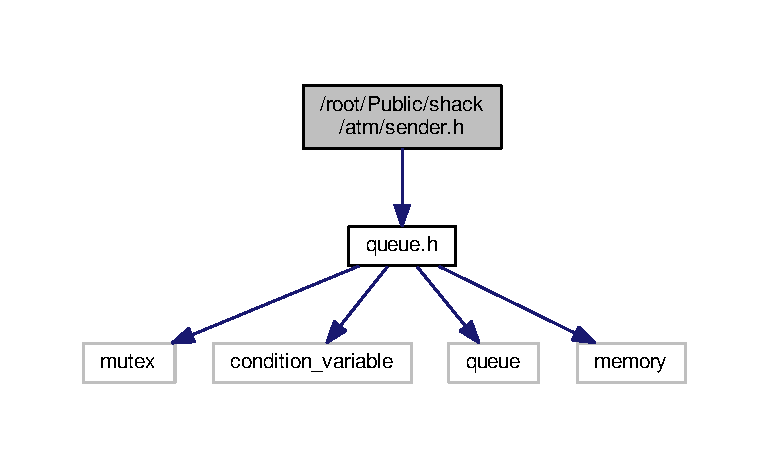
\includegraphics[width=350pt]{sender_8h__incl}
\end{center}
\end{figure}
This graph shows which files directly or indirectly include this file\-:\nopagebreak
\begin{figure}[H]
\begin{center}
\leavevmode
\includegraphics[width=350pt]{sender_8h__dep__incl}
\end{center}
\end{figure}
\subsection*{Classes}
\begin{DoxyCompactItemize}
\item 
class \hyperlink{classmessaging_1_1Sender}{messaging\-::\-Sender}
\end{DoxyCompactItemize}
\subsection*{Namespaces}
\begin{DoxyCompactItemize}
\item 
\hyperlink{namespacemessaging}{messaging}
\end{DoxyCompactItemize}

\hypertarget{template__dispatcher_8cpp}{\section{/root/\-Public/shack/atm/template\-\_\-dispatcher.cpp File Reference}
\label{template__dispatcher_8cpp}\index{/root/\-Public/shack/atm/template\-\_\-dispatcher.\-cpp@{/root/\-Public/shack/atm/template\-\_\-dispatcher.\-cpp}}
}
{\ttfamily \#include \char`\"{}template\-\_\-dispatcher.\-h\char`\"{}}\\*
Include dependency graph for template\-\_\-dispatcher.\-cpp\-:\nopagebreak
\begin{figure}[H]
\begin{center}
\leavevmode
\includegraphics[width=350pt]{template__dispatcher_8cpp__incl}
\end{center}
\end{figure}

\hypertarget{template__dispatcher_8h}{\section{/root/\-Public/shack/atm/template\-\_\-dispatcher.h File Reference}
\label{template__dispatcher_8h}\index{/root/\-Public/shack/atm/template\-\_\-dispatcher.\-h@{/root/\-Public/shack/atm/template\-\_\-dispatcher.\-h}}
}
{\ttfamily \#include \char`\"{}queue.\-h\char`\"{}}\\*
Include dependency graph for template\-\_\-dispatcher.\-h\-:\nopagebreak
\begin{figure}[H]
\begin{center}
\leavevmode
\includegraphics[width=350pt]{template__dispatcher_8h__incl}
\end{center}
\end{figure}
This graph shows which files directly or indirectly include this file\-:\nopagebreak
\begin{figure}[H]
\begin{center}
\leavevmode
\includegraphics[width=350pt]{template__dispatcher_8h__dep__incl}
\end{center}
\end{figure}
\subsection*{Classes}
\begin{DoxyCompactItemize}
\item 
class \hyperlink{classmessaging_1_1TemplateDispatcher}{messaging\-::\-Template\-Dispatcher$<$ Previous\-Dispatcher, Msg, Func $>$}
\end{DoxyCompactItemize}
\subsection*{Namespaces}
\begin{DoxyCompactItemize}
\item 
\hyperlink{namespacemessaging}{messaging}
\end{DoxyCompactItemize}

\hypertarget{withdraw_8h}{\section{/root/\-Public/shack/atm/withdraw.h File Reference}
\label{withdraw_8h}\index{/root/\-Public/shack/atm/withdraw.\-h@{/root/\-Public/shack/atm/withdraw.\-h}}
}
{\ttfamily \#include \char`\"{}sender.\-h\char`\"{}}\\*
{\ttfamily \#include $<$string$>$}\\*
Include dependency graph for withdraw.\-h\-:\nopagebreak
\begin{figure}[H]
\begin{center}
\leavevmode
\includegraphics[width=350pt]{withdraw_8h__incl}
\end{center}
\end{figure}
This graph shows which files directly or indirectly include this file\-:\nopagebreak
\begin{figure}[H]
\begin{center}
\leavevmode
\includegraphics[width=350pt]{withdraw_8h__dep__incl}
\end{center}
\end{figure}
\subsection*{Classes}
\begin{DoxyCompactItemize}
\item 
struct \hyperlink{structWithdraw}{Withdraw}
\item 
struct \hyperlink{structWithdrawOK}{Withdraw\-O\-K}
\item 
struct \hyperlink{structWithdrawDenied}{Withdraw\-Denied}
\item 
struct \hyperlink{structCancelWithdrawal}{Cancel\-Withdrawal}
\item 
struct \hyperlink{structWithdrawProcessed}{Withdraw\-Processed}
\item 
struct \hyperlink{structCardInserted}{Card\-Inserted}
\item 
struct \hyperlink{structDigitPressed}{Digit\-Pressed}
\item 
struct \hyperlink{structClearLastPressed}{Clear\-Last\-Pressed}
\item 
struct \hyperlink{structEjectCard}{Eject\-Card}
\item 
struct \hyperlink{structWithdrawPressed}{Withdraw\-Pressed}
\item 
struct \hyperlink{structCancelPressed}{Cancel\-Pressed}
\item 
struct \hyperlink{structIssueMoney}{Issue\-Money}
\item 
struct \hyperlink{structVerifyPin}{Verify\-Pin}
\item 
struct \hyperlink{structPinVerified}{Pin\-Verified}
\item 
struct \hyperlink{structPinIncorrect}{Pin\-Incorrect}
\item 
struct \hyperlink{structDisplayEnterPin}{Display\-Enter\-Pin}
\item 
struct \hyperlink{structDisplayEnterCard}{Display\-Enter\-Card}
\item 
struct \hyperlink{structDisplayInsufficientFunds}{Display\-Insufficient\-Funds}
\item 
struct \hyperlink{structDisplayWithdrawalCancelled}{Display\-Withdrawal\-Cancelled}
\item 
struct \hyperlink{structDisplayPinIncorrectMessage}{Display\-Pin\-Incorrect\-Message}
\item 
struct \hyperlink{structDisplayWithdrawalOptions}{Display\-Withdrawal\-Options}
\item 
struct \hyperlink{structGetBalance}{Get\-Balance}
\item 
struct \hyperlink{structBalance}{Balance}
\item 
struct \hyperlink{structDisplayBalance}{Display\-Balance}
\item 
struct \hyperlink{structBalancePressed}{Balance\-Pressed}
\end{DoxyCompactItemize}

%--- End generated contents ---

% Index
\newpage
\phantomsection
\addcontentsline{toc}{part}{Index}
\printindex

\end{document}
